\documentclass[12pt,a4paper,twoside]{article}
\usepackage{times}	% Skalierbarer und lesbarer Zeichensatz
\usepackage{ucs}	% Benötigt für Eingabe von unicode-Zeichensätzen
\usepackage[utf8x]{inputenc} % Aktiviert Eingabe von unicode-Zeichensätzen
\usepackage{epsfig}	% Makros zum Einfügen von Grafiken
\usepackage{anysize}	% Makros zum Einstellen der Seitenränder
%\usepackage{makeidx}	% Makros zum Erstellen des Indexes
\usepackage{url}
\usepackage{fancyhdr}
\usepackage{listings}
\usepackage{color}
\usepackage[table]{xcolor}
\usepackage{hyperref}

\marginsize{30mm}{20mm}{20mm}{20mm}  % Seitenränder links, rechts, oben, unten
\parindent0em		% Keine amerikanische Einrückung am Anfang von Paragraphen
\renewcommand{\textfraction}{0.01}
\renewcommand{\floatpagefraction}{0.99}
\renewcommand{\topfraction}{0.99}
\renewcommand{\bottomfraction}{0.99}

\pagestyle{fancy}	% Seitenstil
%\makeindex		% wird für Erstellung von Stichwortverzeichnissen benötigt

\definecolor{linkblue}{rgb}{0,0,0.75}
\definecolor{dkgreen}{rgb}{0,0.66,0}
\definecolor{dkred}{rgb}{0.75,0,0}

\definecolor{dkgrey}{RGB}{184,184,184}
\definecolor{ltgrey}{RGB}{224,224,224}
\definecolor{turquoise}{RGB}{128,255,255}
\definecolor{pink}{RGB}{255,180,240}
\definecolor{dkblue}{RGB}{196,196,240}


\definecolor{ltgreen}{RGB}{192,255,192}
\definecolor{ltyellow}{RGB}{255,255,192}
\definecolor{ltorange}{RGB}{255,224,192}
\definecolor{ltred}{RGB}{255,192,192}

\hypersetup{
    pdftitle={dvdisaster User's Manual},
    pdfauthor={Carsten Gnörlich},
    colorlinks=true,
    linkcolor=linkblue,
    citecolor=linkblue,
    filecolor=linkblue,
    urlcolor=linkblue
}

\newcommand{\projectversion}{0.79.6}

% A link printed in parenthesis

\newcommand{\plnk}[2]{\hyperref[#1]{($\hookrightarrow$ #2)}}

% A text passage used as a link

\newcommand{\tlnk}[2]{\hyperref[#1]{#2}}


% Ende der Voreinstellungen

\newcommand{\paperversion}{{\em for dvdisaster version \projectversion}}

\fancyhead{}
\fancyhead[LE]{\nouppercase{\leftmark}}
\fancyhead[RO]{\nouppercase{\rightmark}}
%\renewcommand{\sectionmark}[1]{\markboth{#1}{#1}}
%\renewcommand{\subsectionmark}[1]{}

%\renewcommand{\footrulewidth}{0.4pt}
\fancyfoot{}
\fancyfoot[LE,RO]{page \thepage\ of \pageref{LastPage}}

\pdftrailerid{dvdisaster}
\pdfsuppressptexinfo=-1
\begin{document}

\definecolor{lightorange}{RGB}{255,224,150}
\pagecolor{lightorange}
\title{The dvdisaster User's Manual}
\author{Carsten Gnörlich\\carsten@dvdisaster.org}
\date{}
\maketitle
\thispagestyle{empty}

\centerline{
\includegraphics[width=40mm]{figures/puzzle.pdf}}

\begin{center}
\paperversion
\end{center}

\bigskip

\begin{abstract}
This is the {\em orange manual}, describing the usage of {\em dvdisaster}, a tool for
creating error correction data (``ecc data'') 
for optical media  such as CD, DVD and BD discs. 
Use cases for creating ecc data, recovering defective media
using ecc data and for general maintenanance of optical 
media are given. 
See \url{http://dvdisaster.org}  for additional resources on
the dvdisaster project, e.g. for the {\em blue} manual (codecs.pdf)
containing a formal specification of the error correction data format.
\end{abstract}

\vfill
\begin{center}
{\em 
Copyright 2008-2018 Carsten Gnörlich.
Verbatim copying and distribution of this entire article is permitted in any medium, 
provided this notice is preserved.}
\end{center}

\newpage
\nopagecolor

% Table of Contents

\tableofcontents
\newpage

\section*{Preface}
\label{preface}

Since the release of dvdisaster 0.79.3\footnote{Version 0.79.4 was never finished
and released.}, nearly five years have passed.
This was partly due to changed circumstances in its
primary developer's life, but there was also a lot of
coding going on behind the scenes. In comparison with its
predecessor, dvdisaster 0.79.5 comes with lots of its
internals being significantly reworked.

\smallskip

The most visible improvement  of dvdisaster 0.79.5 is, of
course, its multithreaded RS03 codec. While it takes
about 62 minutes for protecting a 36 GiB image with RS02
on a mid range PC,
the same task is done with RS03 in less than 7 minutes
using 6 processor cores on the same machine.
On a high end server with at least 16 cores and very good I/O,
this can be done in under a minute. That's quite an
improvement.

RS03 is ready for production use in the current release.
Some non-essential features, especially reworking the
adaptive reading for use with RS03 and multi-threaded
RS03 decoding (media fixing) will be delivered with
the following dvdisaster releases.

\smallskip

Other parts of the project had to be changed or even
discontinued. A software project lives on development
and continuous releases; else the
project will eventually die. In this respect, dvdisaster
was very endangered in the last few years.
To prevent this from happening again, most effort
is now directed into source code development;
everything else is delegated or discontinued.
Source code development basically means making
the GNU/Linux version, which provides the code base
for all other versions, and the FreeBSD and NetBSD ports,
which are very easily derived from the GNU/Linux code.
This is not the case for the Mac OS and Windows ports,
which are, unfortunately, \tlnk{qa-discontinued-os}{discontinued} as of now.

Another feature which has to go are the separate
stable and development releases.
Starting with this version, all dvdisaster releases
are considered production quality, so there is no
need for different branches anymore.

\smallskip

Maintaining the multi-lingual online documentation, which
also served as the project home page, did also prove to
be too time consuming. The project home page has
been changed into a simple download platform for
the project sources. It is now directed at package
maintainers who will create and pass on binaries
for the GNU/Linux, FreeBSD and NetBSD distributions.

The program documentation, which you are reading
right now, is provided in PDF format which is much
easier to author than the HTML version. The only
language available is English. Most parts of this
manual have been adapted from the old online
documentation, so it still feels more like a website
than a book. While hyperlinks are not as usable in PDF
as in HTML, they have been kept in this document to
stress that it is intended to be used as an online reference.
So please do our environment a favour and do not print
this manual. It is not meant to be read
from front cover to back cover, anyways.

\smallskip

Okay, enough ranting already. May dvdisaster be helpful
in protecting and recovering your valuable data,
and thanks for using it!

\bigskip

{\em -- -- cg, August 2015}



\newpage

\section{Overview}

\paragraph{The challenge: Optical media eventually fail.} Optical media (CD,DVD,BD) keep their data only for a finite time (typically for many years). 
After that time, data loss develops slowly with read errors growing from the outer 
media region towards the inside. 

\paragraph{The dvdisaster solution: Archival with data loss protection.}
dvdisaster complements optical media \plnk{qa-technical-media}{supported media} with
error correction data
in a way that they are fully recoverable 
even after some read errors have developed. 
This enables you to rescue the complete data to a new medium.

Error correction data, in short ``ecc data'',  is either added to the medium 
or kept in separate error correction files. dvdisaster works at the image level 
so that the recovery does not depend on the file system of the medium. 
The maximum error correction capacity is user-selectable.

\subsection{Common misunderstandings about dvdisaster}

Before we describe in detail what dvdisaster can do, let's first clarify what it can't:

\paragraph{dvdisaster can not make defective media readable again.}
Like a conventional backup, error correction data must be created from 
a fully functional optical medium - {\em you can not backup data which has already
been lost}. When the optical medium develops defective sectors at a later time,
those defective sectors are restored by re-calculating them from the ecc data. 
This won't make the defective medium working again, but will produce a new iso 
image which can be written to a new medium. 

As said before, ecc data can not be created from already defective media.
Although unreadable sectors can not be recovered in that case, dvdisaster
might still be helpful in extracting the remaining readable portions of the medium. 

\paragraph{It's not a ripping tool.} If you want a tool for copying
protected media, you're looking at the wrong place. Such functions are
outside the scope of dvdisaster's internal design and goals.
Contrary to some myths saying otherwise: dvdisaster contains 
no hidden program fragments or switches for reading protected discs.
Check the source code for yourself if you don't trust me.

 
\subsection{How to use this manual}

Many users just want to see some examples of solving typical tasks. Flip over
to the \tlnk{howtos}{Typical applications section} in that case. 

\smallskip

The remainder of this section gives an example of recovering a defective medium including
screen shots, relates using ecc data to performing quality scans and full backups,
and summarizes the pro and con of dvdisaster.

\smallskip

The \tlnk{download}{downloads} section provides a link to the download site,
summarizes the \tlnk{download-requirements}{system requirements},
and clarifies that you can get and use dvdisaster as
\tlnk{download-terms}{free software, at no cost and while keeping
your full privacy}.

\smallskip

There is also a chapter containing \tlnk{qa}{general questions and answers},
\tlnk{qa-technical}{technical questions and answers}, 
and explanations of \tlnk{qa-error}{error messages}.

\smallskip

The \tlnk{background}{background information} section provides details on
the \tlnk{background-properties}{properties of the error correction},
the difference between \tlnk{background-image-level}{image level and file level data recovery},
the \tlnk{background-methods}{RS01, RS02 and RS03 error correction methods},
the \tlnk{background-linear}{linear}
and \tlnk{background-adaptive}{adaptive} reading strategies,
some \tlnk{background-read-errors}{remarks on how media read errors come into existance},
and finally a few \tlnk{background-eccfile-storage}{hints for storing error correction files}.

\smallskip

As not all optical disc burning software may be compatible with dvdisaster,
you might want to check
the \tlnk{burning-compatibility}{compatibility table} and the additional
information provided with it.

\smallskip

If you encounter a defect (programming error) or
incompatibility with a certain (drive) hardware and software setup,
please see the \tlnk{reporting-defects}{reporting defects} section.

%\newpage

\subsection{Example of the error correction}

\begin{figure}[h]
\centerline{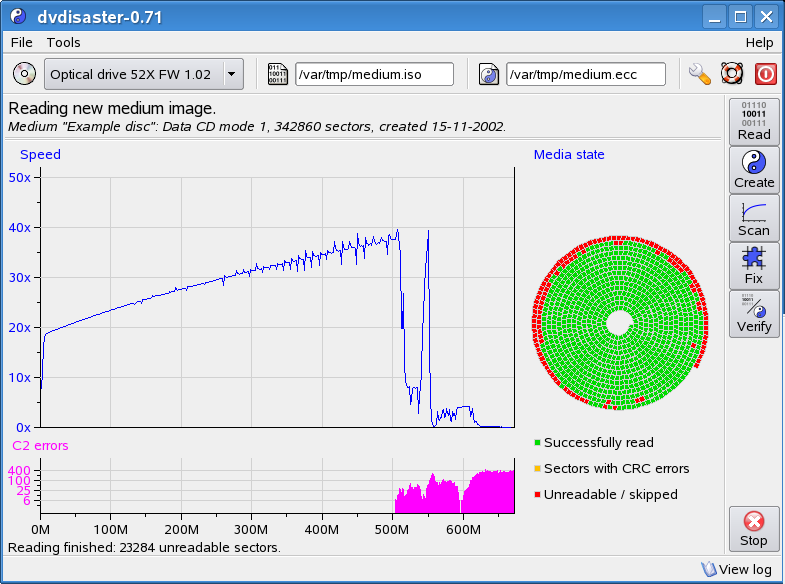
\includegraphics[width=\textwidth]{screenshots/recover-linear.png}}
\caption{Reading a defective medium.}  
\label{recover-linear}
\end{figure}

\paragraph{Recovery of aged media.} 
The medium processed here has become discolored and partly unreadable in its outer region.
A reading attempt yields about 23.600 unreadable sectors of 360056 sectors total;
resulting in about 6,6\% defective sectors. Figure \ref{recover-linear} shows the
dvdisaster window after the reading attempt. The distribution of reading speed and
read errors over the medium is graphically shown.
The still readable sectors are stored in an ISO image called {\em medium.iso}.

\begin{figure}[t]
\centerline{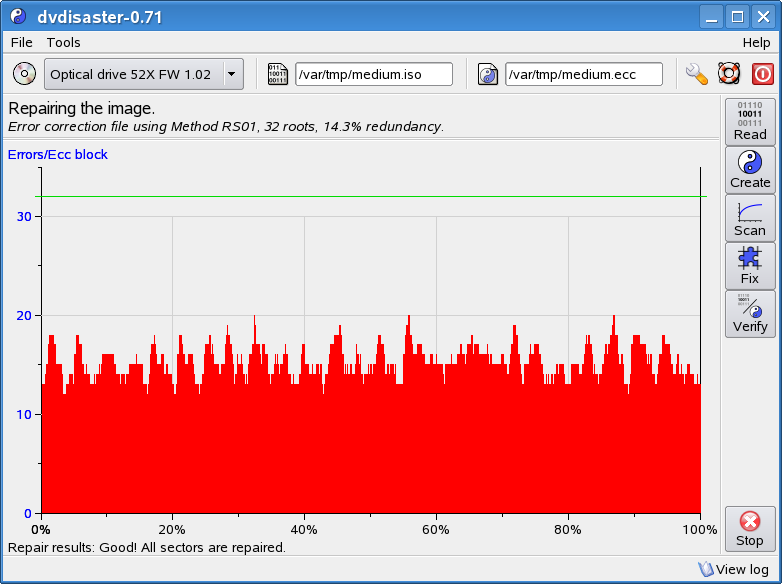
\includegraphics[width=\textwidth]{screenshots/fix-image.png}}
\caption{Repairing the defective image.}  
\label{fix-image}
\end{figure}

\paragraph{Repairing the defective image.} 
The image which has been just read is incomplete since about 23.600 sectors could
not be read. These sectors are now reconstructed using the error correction data
created with dvdisaster. During the recovery a maximum of 20 errors per error
correction block is encountered (see figure \ref{fix-image}).
This results in a peak error correction load of
63\%, meaning that this degree of damage is handled well by error correction data
created with default settings. The recovered image can now be written to a new medium.

\paragraph{Recovery needs error correction data:}
The recovery process described above uses error correction (``ecc'') data.
Think of this data as a special form of backup data (it needs less space
than a normal backup, though). Like an ordinary backup, the ecc data needs
to be created before the medium goes defective.

So if you have a defective medium but never created ecc data for it, you will
not be able to recover the defective sectors (23.600 in the above example).
The data located at the end of the medium will be lost, while you will probably
be able to extract some files which are located at the beginning of the medium.
\newpage

\subsection{dvdisaster as a complement to quality scans}

\tlnk{qa-quality-scans}{Quality scans}, e.g. C2 error or PI/PO scans are a valuable tool
for testing the results of the media writing process.

\smallskip

But quality scans are {\bf not} a reliable means of
{\bf predicting the lifetime} of optical media.
Consider we are looking for the right time to copy a worn-out medium onto a new one:

\begin{itemize}
\item Too early: Copying media because of a bad quality scan is cost-ineffective.
  Sometimes such media remain readable much longer than expected.
\item Too late: When the quality scan reveals unreadable sectors some data has already been lost.
\item Right before the medium fails: The ideal case, but how to tell?
\end{itemize}

However, we could do it the dvdisaster way:

\begin{itemize}
\item \tlnk{howto-ecc}{Create error correction data} for the medium.
\item \tlnk{howto-scan}{Scan the medium} regularly. Use it until the first read errors occur.
\item \tlnk{howto-recover}{Recover} the read errors using the error correction data.
  Write the recovered image to a new medium.
\end{itemize}

\subsection{Error correction data vs. full backup}
\label{overview-backup}

\paragraph{A conventional backup strategy}$\!\!\!\!\!$ would be making one or 
more copies of the optical medium. This has a few advantages:
Copying a medium is fast, and having two (or more) working copies
available can be convenient, especially when working at different
locations.

\smallskip

The disadvantage of this approach is that it guards only against
incidental damage, but not against general aging. It is not helpful
to have ten copies which all decay in a similar manner. If all 
ten copies are unreadable in the outermost region after a few years,
data loss has occurred even though we were spending 900\% of the
original storage capacity for the backup.

\paragraph{Ecc data behaves differently}$\!\!\!\!\!$ since it is not a verbatim
copy of the original data. It is a mathematical scheme working like
this: Give me any 80\% of the original data and I will be able to
reconstruct the missing 20\%, regardless of {\em where} the 20\%
are missing (whether at the beginning or at the end, maybe in between - doesn't
matter). Incidentally, there is a strong relationship between 
being able to reconstruct a missing percentage of the original data 
and the size of the ecc data: If the ecc data is 20\% of the size of
the original data, it can roughly recover up to 20\% of missing data;
with ecc data being 30\% of the original size up to 30\% can be recovered
and so on. But this relationship isn't even the greatest advantage
of the ecc data; the ``regardless of where the defects are'' is the big deal.

\smallskip

Let's assume we want to have a 100\% protection of a specific 4 GiByte 
DVD. Then we create another DVD containing 4 GiBytes of ecc data. 
At a later date, both DVDs decay and the last 30\% of both become
unreadable. Since we have still 70\% of the original data and of the
ecc data, everything is fine! We can still reconstruct the original 
data from them; using the second DVD for ecc data is much more
efficient than creating a second copy on it. In fact putting another
copy on the second DVD would not have saved us from a 30\% data loss.

\smallskip

We can even make some assumptions about our media. Maybe we expect
that even a defective medium will not lose more than 15\% of its data 
(don't take my word on it). And we make sure that ecc data will be saved
on a different type of medium which is considered to have a longer life than optical
media. Then creating ecc data with a recovery rate of 20\% (always
leave a safety margin) should suffice our needs. 
This would yield a reasonable data protection
while spending only an additional 20\% of storage for it. 

\smallskip

This is not to say that ecc data is the final answer to all
archiving means, but when used well, it can be much more
efficient and secure than a simple backup strategy. See also the
\tlnk{bigpicture-backup}{``Big Picture'' section} for a continued
ecc data vs. full backup discussion.

\subsection{Pro and con of dvdisaster}

To summarize from the previous sub sections:

\bigskip
{\bf Advantages of using dvdisaster:}

\begin{itemize}
\item {\bf Protects} against aging and accidental medium damage (within certain limits).
\item \tlnk{howto-scan}{Read error tests} run {\bf faster} than quality scans; up to full reading speed depending on the drive.
\item {\bf Cost-effective:} Media must be replaced with a new copy only when they are really defective.
\item {\bf Space-efficient:} Ecc data requires less space than a full backup under most scenarios.
\end{itemize}

\bigskip
{\bf Limitations of using dvdisaster:}

\medskip

You need a backup and testing strategy and at least 15\% of additional storage.

\begin{itemize}
\item Error correction data {\bf must be created before the medium fails}, preferably at the same time the medium is written.
\item Error correction data requires {\bf additional storage space} either on the protected medium or by using additional media. Using the standard settings the additional storage space amounts to 15\% of the original data size (approx. 700MiB for a full 4.7GiB DVD).
\item No guaranteed protection against data loss as limits and statistical properties of the
  error correction may be exceeded with extremely bad luck.
\end{itemize}

\bigskip

See also the \tlnk{background}{collection of background information} to learn
more about the functioning of dvdisaster.

\newpage

\newcommand{\goodcd}{
\includegraphics[width=15mm]{icons/good-cd.png}}
\newcommand{\badcd}{
\includegraphics[width=16mm]{icons/bad-cd.png}}
\newcommand{\badcdone}{
\includegraphics[width=19mm]{icons/bad-cd1.png}}
\newcommand{\goodimage}{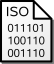
\includegraphics[width=13mm]{icons/good-image.png}}
\newcommand{\goodimagetwo}{
\includegraphics[width=13mm]{icons/good-image2.png}}
\newcommand{\badimage}{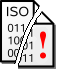
\includegraphics[width=15mm]{icons/bad-image.png}}
\newcommand{\oldcd}{
\includegraphics[width=15mm]{icons/old-cd.png}}
\newcommand{\oldimage}{
\includegraphics[width=15mm]{icons/old-image.png}}
\newcommand{\augmentedcd}{
\includegraphics[width=15mm]{icons/augmented-cd.png}}
\newcommand{\eccfile}{
\includegraphics[width=13mm]{icons/ecc-file.png}}
\newcommand{\backupone}{
\includegraphics[width=18mm]{icons/backup1.png}}
\newcommand{\backuptwo}{
\includegraphics[width=19mm]{icons/backup2.png}}
\newcommand{\rightarr}{
\includegraphics[width=11mm]{icons/right-arrow.png}}
\newcommand{\downarr}{
\includegraphics[height=11mm]{icons/down-arrow.png}}
\newcommand{\downforkarr}{
\includegraphics[height=11mm]{icons/down-fork-arrow.png}}
\newcommand{\rdiagarr}{
\includegraphics[height=9mm]{icons/rdiag-arrow.png}}
\newcommand{\ldiagarr}{
\includegraphics[height=9mm]{icons/ldiag-arrow.png}}
\newcommand{\joinarr}{
\includegraphics[height=11mm]{icons/join-arrow.png}}

\newcommand{\slotin}{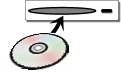
\includegraphics[height=17mm]{icons/slot-in.png}}
\newcommand{\filemanager}{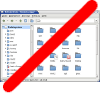
\includegraphics[height=20mm]{icons/filemanager.png}}
\newcommand{\selectdrive}{
\includegraphics[height=10mm]{icons/select-drive.png}}
\newcommand{\selectimage}{
\includegraphics[height=8.5mm]{icons/select-image.png}}
\newcommand{\selectecc}{
\includegraphics[height=8.5mm]{icons/select-ecc.png}}
\newcommand{\scanicon}{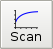
\includegraphics[height=13mm]{icons/scan-icon.png}}
\newcommand{\readicon}{
\includegraphics[height=13mm]{icons/read-icon.png}}
\newcommand{\createicon}{
\includegraphics[height=13mm]{icons/create-icon.png}}
\newcommand{\fixicon}{
\includegraphics[height=13mm]{icons/fix-icon.png}}
\newcommand{\verifyicon}{
\includegraphics[height=13mm]{icons/verify-icon.png}}
\newcommand{\stopicon}{
\includegraphics[height=13mm]{icons/stop-icon.png}}
\newcommand{\logicon}{
\includegraphics[height=6mm]{icons/log-icon.png}}

\section{Typical applications - HowTos}
\label{howtos}

dvdisaster is a complex tool which would require a book of a few hundred pages
to cover all of its features. Since we are currently lacking the resources for
doing such a book (and you might be short on reading time also) we will take
a different approach in this section. First we demonstrate how the different functions
of dvdisaster work together. Then we describe common tasks and provide
step by step instructions for solving them. In most cases following these steps
will be all you need to do. At the end of each instruction set a discussion
of further configuration options is included for advanced users.

\subsection{Symbols used in this document}

Working with dvdisaster requires certain combinations of optical media,
media images and error correction data. Check out the following symbols to
find out what you will need for the respective tasks:

\paragraph{Medium} (a CD for example):

\bigskip

\begin{tabular}{ccl}
  \begin{minipage}{20mm}
  \centerline{\goodcd}
  \end{minipage}
  &
  \begin{minipage}{20mm}
  \centerline{\badcd}
  \end{minipage}
  &
  \begin{minipage}{93mm}
  These symbols indicate whether processing a medium is part of the
  respective task, and if the medium needs to be completely error free or may already be damaged. 
  \end{minipage}\\
  & & \\

  good medium & bad medium & \\
  ({\bf no} read errors) & ({\bf with} read errors) & \\
\end{tabular}

\paragraph{Medium image} (ISO image of a medium stored on the hard disk):

\bigskip

\begin{tabular}{ccl}
  \begin{minipage}{20mm}
  \centerline{\goodimage}
  \end{minipage}
  &
  \begin{minipage}{20mm}
  \centerline{\badimage}
  \end{minipage}
  &
  \begin{minipage}{93mm}
    Some functions do not work directly with the medium, but with an ISO image
    on hard disk instead. Depending on the condition of the respective medium the
    image may be complete or incomplete.
  \end{minipage}\\
  & & \\

  complete image & incomplete image & \\
  (made from  & (made from & \\
  good medium) & bad medium) & \\
\end{tabular}

\paragraph{Error correction data}\quad

\bigskip

\begin{tabular}{ccl}
  \begin{minipage}{20mm}
  \centerline{\augmentedcd}
  \end{minipage}
  &
  \begin{minipage}{20mm}
  \centerline{\eccfile}
  \end{minipage}
  &
  \begin{minipage}{93mm}
    Recovering media images by using error correction data is the
    key feature of dvdisaster. These symbols show whether error
    correction data is required.
  \end{minipage}\\
  & & \\

  Medium containing & Separate error& \\
  error correction data   & correction file & \\
\end{tabular}


\subsection{The big picture - understanding dvdisaster}

In this sub section we are getting a basic understanding
of dvdisaster:

\begin{itemize}
\item It is important to understand that dvdisaster works similar
  to a \tlnk{bigpicture-backup}{conventional backup} in some
  regards, but that there are also important differences.
\item The general
  \tlnk{bigpicture-ecc}{idea of the error correction} is explained.
\item Jane demonstrates the
  \tlnk{bigpicture-goodusage}{proper usage of dvdisaster}.
  She will create error correction data in advance and is
  therefore able to recover all data when her media become defective.
\item However you should \tlnk{bigpicture-badusage}{not follow the way}
  of Joe. He does not use error correction data and finds out that
  his defective media are not recoverable even after multiple
  reading passes. As a consequence he loses data from a defective medium.
\end{itemize}

Of course these stories are purely fictional and any similarities with existing persons or situations are purely conincidental. 

\subsubsection{A comparison of dvdisaster with conventional backup}
\label{bigpicture-backup}

dvdisaster stores data on optical discs in a way that the data
is fully recoverable even after the medium has developed some read errors.
The method employed in dvdisaster uses less storage space (or additional media)
than a full backup would do. Before using dvdisaster it is important to
understand the similarities and differences between dvdisaster and a
conventional (full) backup.

\bigskip

Let's first consider how a conventional backup scheme works:

\bigskip

\begin{tabular}{cccl}
  \begin{minipage}{20mm}
  \centerline{\backupone}
  \end{minipage}
  &
  \begin{minipage}{12mm}
  \centerline{Copy}\par
  \centerline{\rightarr}
  \end{minipage}
  &
  \begin{minipage}{20mm}
  \centerline{\backuptwo}
  \end{minipage}
  &
  \begin{minipage}{92mm}
    An existing medium (1) is copied onto a backup medium (2).
  \end{minipage}\\

  \begin{minipage}{20mm}
  \centerline{\downarr}
  \end{minipage}
  &
  &
  \begin{minipage}{20mm}
  \centerline{\downarr}
  \end{minipage}
  & \\[4mm]

  \begin{minipage}{20mm}
  \centerline{\badcdone}
  \end{minipage}
  &
  &
  \begin{minipage}{20mm}
  \centerline{\backuptwo}
  \end{minipage}
  &
  \begin{minipage}{92mm}
    If any one of the two media is damaged afterwards,
    we still have an intact medium left.
  \end{minipage}\\
\end{tabular}

\bigskip

There are actually some cases where it is important to keep a
second copy of an optical disc: One medium might get lost,
burst while spinning in the drive, or it may be destroyed due
to mishandling. However such cases of complete data loss are
rare as long as optical media are handled properly.

\smallskip

It is more likely that the medium starts to gradually lose data
after a few years - a nearly unavoidable aging process.
When the medium is regularly used (or scanned for defects)
the data loss will typically be noticed after 5\% to 10\% of
the medium have already become unreadable. At this point
the medium is unusable as a whole, but maybe 90\% of
it is still readable. {\em On the other hand a full backup copy
of the medium is not required; we simply need a method for
recovering the missing 10\% of data.}

\smallskip

This is where dvdisaster comes into play. Consider this:

\bigskip

\begin{tabular}{cccl}
  \begin{minipage}{20mm}
  \centerline{\goodcd}
  \end{minipage}
  &
  \begin{minipage}{12mm}
    \centerline{Create}\par
    \centerline{\rightarr}\par
    \centerline{ECC}
  \end{minipage}
  &
  \begin{minipage}{20mm}
  \centerline{\eccfile}
  \end{minipage}
  &
  \begin{minipage}{92mm}
    This time we do not make a full backup. dvdisaster is used
    to create error correction data (``ECC'') which can recover
    up to 20\% of a degraded medium. The value of 20\% was
    chosen to have a safety margin over the expected data loss
    of 5-10\%. 
  \end{minipage}\\

  \begin{minipage}{20mm}
  \centerline{\downarr}
  \end{minipage}
  &
  &
  \begin{minipage}{20mm}
  \centerline{\downarr}
  \end{minipage}
  & \\[4mm]

  \begin{minipage}{20mm}
  \centerline{\badcd}
  \end{minipage}
  &
  &
  \begin{minipage}{20mm}
  \centerline{\eccfile}
  \end{minipage}
  &
  \begin{minipage}{92mm}
    Wenn the medium fails at a later time, its contents are
    recovered from its still readable parts and from the
    error correction data.
  \end{minipage}\\[8mm]

  \begin{minipage}{20mm}
  \mbox{80\%\rdiagarr}
  \end{minipage}
  &
  &
  \begin{minipage}{20mm}
  \mbox{\ldiagarr20\%}
  \end{minipage}
  &
  \begin{minipage}{92mm}
    For a successful recovery at least 80\% of the data must
    still be readable from the medium, and the remaining 20\% are
    recalculated from the error correction data.
  \end{minipage}\\[7mm]

  \multicolumn{3}{c}{\begin{minipage}{20mm}\centerline{\goodimage}\end{minipage}}
  &
  \begin{minipage}{92mm}
  The completely recovered data is now available as an ISO image
  on the hard drive (the medium remains defective as physical
  data loss is irrevocable).
  \end{minipage}\\[8mm]

  \multicolumn{3}{c}{\begin{minipage}{20mm}\centerline{\downarr}\end{minipage}}
  &
  \begin{minipage}{92mm}
    Write the image to a blank medium using your favourite
    optical disc authoring software.
  \end{minipage}\\[6mm]

  \multicolumn{3}{c}{\begin{minipage}{20mm}\centerline{\goodcd}\end{minipage}}
  &
  \begin{minipage}{92mm}
  You now have a new error-free medium.
  \end{minipage}\\
\end{tabular}

\bigskip

As you have seen the data recovery took more steps then
doing a conventional backup and restore. So let's summarize the pros
and cons of dvdisaster compared with conventional backup:

\bigskip

\paragraph{Advantages}\quad 	

\begin{itemize}
\item dvdisaster uses less storage. When using error correction
  data with a 20\% recovery capability, protecting 5 media
  requires only one additional medium for the ECC data.
\item  Since all media will eventually age and start losing data in
  similar places (typically in the outermost region),
  doing a 1:1 copy might not help at all. Both copies may turn
  out defective in the same places after a few years.
\end{itemize}

\paragraph{Similarities}\quad

\begin{itemize}
\item Both backup copies and error correction data must
  be created before the master disc fails. You can't create
  them from an already defective medium.
\end{itemize}

\paragraph{Disadvantages}

\begin{itemize}
\item If the recovery capability of the error correction
  data is exceeded (or the medium gets lost), no data
  can be recovered! Especially take note that error
  correction data with a repair rate of 20\% together
  with a 75\% readable medium does not result
  in 95\% recovery. In that case, nothing beyond the 75\% readable
  data from the medium can be recovered.
\end{itemize}

Some of these points are also discussed in
\tlnk{overview-backup}{Error correction data vs. full backup} in the
``Overview'' section, from a slightly different view point.

\subsubsection{The idea behind the error correction}
\label{bigpicture-ecc}

\bigskip

\begin{tabular}{cccl}
    \begin{minipage}{20mm}
  \centerline{\badcd}
  \end{minipage}
  &
  &
  \begin{minipage}{20mm}
  \centerline{\eccfile}
  \end{minipage}
  &
  \begin{minipage}{104mm}
    The example from the previous page told us how dvdisaster
    reconstructs data by using the still readable parts
    of the medium together with the error correction data.
  \end{minipage}\\[8mm]

  \begin{minipage}{20mm}
  \mbox{80\%\rdiagarr}
  \end{minipage}
  &
  &
  \begin{minipage}{20mm}
  \mbox{\ldiagarr20\%}
  \end{minipage}
  & \\[-3mm]

  \multicolumn{3}{c}{\begin{minipage}{20mm}\centerline{\goodimage}\end{minipage}}
  &
  \begin{minipage}{104mm}
    In order to get the most out of dvdisaster a basic
    understanding of the error correction method is helpful.
    And while we are at it we can refute a misunderstanding we
    sometimes hear - the error correction data is not simply a
    copy of the last 20\% data sectors. That'd really be a cheap shot ;-)
  \end{minipage}\\[8mm]
\end{tabular}

\paragraph{Example: Anna's desk drawer PIN}\quad

Anna has got a desk whose drawers can only be opened after entering
the numbers "8 6 2 3" into a code lock. Since the drawers
do not contain any sensitive information she decides
to note down the numbers directly on the desktop:

\bigskip


\includegraphics[height=11mm]{figures/pin.pdf}

Anna is cautious and expects one of the numbers to become
unreadable by accidentally pouring ink over it.
Therefore she also notes down the sum of the four
numbers (the ``+'' and ``='' signs have only be added
for clarity):

\bigskip


\includegraphics[height=12mm]{figures/pin-sum.pdf}

After a while one of the numbers indeed gets covered by an ink spot:

\bigskip


\includegraphics[height=13mm]{figures/pin-ink.pdf}

But this is not a problem as Anna can re-calculate the missing number x by rearranging the still readable parts of the equation:

\medskip

\verb|8 + x + 2 + 3 = 19|, \quad hence

\smallskip

\verb|x = 19 - 8 - 2 - 3|, \quad and therefore \verb|x = 6|.

\bigskip

It is easily seen that any one of the original five numbers
can be recovered from the remaining four.
The example also demonstrates some important properties
of the error correction: 

\bigskip

\begin{tabular}{cl}
\begin{minipage}{0.40\textwidth}
  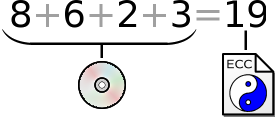
\includegraphics[height=28mm]{icons/ecc-example.png}
\end{minipage}
  &
\begin{minipage}{0.56\textwidth}
  For a given set of data (e.g. the numbers ``8 6 2 3'') additional
  error correction data (e.g. the sum ``19'') can be created so
  that a lost datum can be re-calculated from the remaining data.

  \smallskip
  
  The same principle is used in dvdisaster; the protected sequence
  of numbers is nothing else than the ISO image of an optical disc.
\end{minipage}
\end{tabular}

\bigskip

The concept of {\bf redundancy} can be explained as follows:

\begin{itemize}
\item  One ``error correction number'' is calculated for four input
  numbers. 1 of 4 (or 1/4) relates to a redundancy of 25\%.
\item  From one error correction number we can re-calculate exactly
  one missing number, or at most 25\% of data. The redundancy
  is equivalent to the maximum capacity of the error correction.
\item  Additional storage required for the error correction data is
  also determined by the redundancy (again, 25\% in the example).
\end{itemize}

dvdisaster uses the term of redundancy accordingly.
In addition please observe that

\begin{itemize}
\item  no data can be recovered when the data loss exceeds the
  redundancy (the equation in the example can not be solved for
  two or more unknowns).
\item the error correction data must be calculated at a
  point in time where all data is still present / readable.
\end{itemize}
  
The above shown example does not generalize into an error correction
scheme for recovering more than one missing data value. To do so a
more powerful equation system is needed which can be solved for more
than one missing value. dvdisaster uses a Reed-Solomon code which
does have such properties; however the required math is usually
not taught in school. Interested readers are therefore referred
to the respective books in coding theory. 

\newpage
\subsubsection{Using dvdisaster the right way}
\label{bigpicture-goodusage}

Let's demonstrate how Jane uses dvdisaster.

\bigskip

\begin{tabular}{rccl}
  10. Feb. 2009 &
  \begin{minipage}{16mm}\centerline{\goodcd}\end{minipage} &
  &
  \begin{minipage}{88mm}
    Jane creates a new CD with important data.
  \end{minipage}\\[8mm]

  &
  \begin{minipage}{16mm}\centerline{\goodcd}\end{minipage} &
  \begin{minipage}{16mm}\centerline{\eccfile}\end{minipage}  &
  \begin{minipage}{88mm}
    To protect the CD from data loss she creates
    \tlnk{howto-eccfile}{error correction data} with dvdisaster.
    She keeps both kinds of data for later usage.
  \end{minipage}\\[8mm]
  \hline

14. May 2010 &
  \begin{minipage}{16mm}\centerline{\goodcd}\end{minipage} &
  \begin{minipage}{16mm}\centerline{\eccfile}\end{minipage}  &
  \begin{minipage}{88mm}
    \vspace*{3mm}
    Jane knows that during daily use not all data of
    her CD might be accessed. So after a year has passed
    she \tlnk{howto-scan}{scans the CD for read errors} to make sure that
    it has not developed any defects in seldom used data regions.
    However after one year the CD is still perfectly readable.
    \vspace*{3mm}
  \end{minipage}\\[8mm]
  \hline

19. Aug 2012 &
  \begin{minipage}{16mm}\centerline{\badcd}\end{minipage} &
  \begin{minipage}{16mm}\centerline{\eccfile}\end{minipage}  &
  \begin{minipage}{88mm}
    \vspace*{3mm}
    Two more years have passed and Jane notices that
    some data on the CD is no longer readable.
    A \tlnk{howto-scan}{scan for read errors} confirms
    that the CD has become defective due to aging.
  \end{minipage}\\[8mm]

  \tlnk{howto-recover-read}{read} &
  \begin{minipage}{16mm}\centerline{\downarr}\end{minipage} &
  &
  \\[8mm]

  &
  \begin{minipage}{16mm}\centerline{\badimage}\end{minipage} &
  \begin{minipage}{16mm}\centerline{\eccfile}\end{minipage}  &
  \begin{minipage}{88mm}
    \vspace*{3mm}
    Jane uses dvdisaster
    to \tlnk{howto-recover-read}{read as much sectors as possible} from
      the defective CD into an ISO image.
  \end{minipage}\\[8mm]

  \tlnk{howto-recover-fix}{reconstruct} &
  \multicolumn{2}{c}{\begin{minipage}{32mm}\hspace*{5mm}\joinarr\end{minipage}} &
  \\[8mm]

  &
  \begin{minipage}{16mm}\centerline{\goodimage}\end{minipage} &
  \begin{minipage}{16mm}\centerline{\eccfile}\end{minipage}  &
  \begin{minipage}{88mm}
    By using the error correction data
    Jane \tlnk{howto-recover-fix}{recovers the missing parts} in
    the ISO image. 
  \end{minipage}\\[8mm]

  Write new CD&
  \begin{minipage}{16mm}\centerline{\downarr}\end{minipage} &
  &
  \\[8mm]

  &
  \begin{minipage}{16mm}\centerline{\goodcd}\end{minipage} &
  \begin{minipage}{16mm}\centerline{\eccfile}\end{minipage}  &
  \begin{minipage}{88mm}
    Jane writes a new CD from the recovered ISO image.
    She keeps the error correction data for the new CD
    as it may also become defective in the future.
  \end{minipage}\\[8mm]
\end{tabular}

\newpage
\subsubsection{Using dvdisaster the wrong way}
\label{bigpicture-badusage}

Joe bets on his media keeping their content without additional protection.

\bigskip

\begin{tabular}{rccl}
  10. Feb. 2009 &
  \begin{minipage}{16mm}\centerline{\goodcd}\end{minipage} &
  \begin{minipage}{16mm}\centerline{\goodcd}\end{minipage} &
  \begin{minipage}{88mm}
    Joe creates two CDs containing important data.
    But he does not make any provisions against data loss on those media.
  \end{minipage}\\[8mm]

  \hline
  
  \vspace*{3mm}
  14. May. 2010 &
  \begin{minipage}{16mm}
    \vspace*{3mm}
    \centerline{\goodcd}\end{minipage} &
  \begin{minipage}{16mm}
    \vspace*{3mm}
    \centerline{\goodcd}\end{minipage} &
  \begin{minipage}{88mm}
    Joe uses his CDs regularly. After one year they are
    still perfectly readable.
  \end{minipage}\\[4mm]

  \hline

  \vspace*{3mm}
  19. Aug. 2012 &
  \begin{minipage}{16mm}
    \vspace*{3mm}
    \centerline{\badcd}\end{minipage} &
  \begin{minipage}{16mm}
    \vspace*{3mm}
    \centerline{\goodcd}\end{minipage} &
  \begin{minipage}{88mm}
    After two more years Joe notices that some data
    on one CD is no longer readable.
  \end{minipage}\\[-1mm]

  \tlnk{howto-scan}{scan} &
  \begin{minipage}{16mm}\centerline{\downarr}\end{minipage} &
  \begin{minipage}{16mm}\centerline{\downarr}\end{minipage} &
  \\[-1mm]

  20. Aug. 2012 &
  \begin{minipage}{16mm}
    \centerline{\badcd}\end{minipage} &
  \begin{minipage}{16mm}
    \centerline{\badcd}\end{minipage} &
  \begin{minipage}{88mm}
    Joe downloads dvdisaster and performs
    a \tlnk{howto-scan}{read error scan}.
    He finds out that the CD contains 25000 unreadable sectors.
    A scan of the second CD reveals that it has developed 1500
    unreadable sectors gone unnoticed so far. 
  \end{minipage}\\[-2mm]

  \tlnk{howto-recover}{reading} &
  \begin{minipage}{16mm}\centerline{\downarr}\end{minipage} &
  \begin{minipage}{16mm}\centerline{\downarr}\end{minipage} &
  \\[5mm]

  21. Aug. 2012 &
  \begin{minipage}{16mm}
    \centerline{\badimage}\end{minipage} &
  \begin{minipage}{16mm}
    \centerline{\badimage}\end{minipage} &
  \begin{minipage}{88mm}
    Joe uses dvdisaster to read as much sectors as
    possible from the defective media. But since he
    does not have error correction data there is no way
    of recalculating the unreadable sectors.
  \end{minipage}\\[6mm]

  \begin{minipage}{20mm}
    many reading attempts
  \end{minipage}
    &
  \begin{minipage}{16mm}\centerline{\downarr}\end{minipage} &
  \begin{minipage}{16mm}\centerline{\downarr}\end{minipage} &
  \\[-10mm]

  05. Sep. 2012 &
  \begin{minipage}{16mm}
    \centerline{\badimage}\end{minipage} &
  \begin{minipage}{16mm}
    \centerline{\goodimage}\end{minipage} &
  \begin{minipage}{88mm}
    Joe takes advantage of dvdisaster's feature to complete images
    through multiple reading passes. He moves the defective images
    to several computers to perform reading attempts with
    different drives. After two weeks of trying at least all
    missing sectors from the second CD have been read. However
    on the first CD still 21000 sectors remain unreadable by any
    drive he tried.
  \end{minipage}\\[-4mm]

  \begin{minipage}{25mm}
    only one CD recovered
  \end{minipage}
    &
  \begin{minipage}{16mm}\centerline{\downarr}\end{minipage} &
  \begin{minipage}{16mm}\centerline{\downarr}\end{minipage} &
  \\[-2mm]

  06. Sep. 2012 &
  \begin{minipage}{16mm}
    \centerline{\badcd}\end{minipage} &
  \begin{minipage}{16mm}
    \centerline{\goodcd}\end{minipage} &
  \begin{minipage}{88mm}
    Joe dismisses the first CD as unrecoverable and
    considers himself lucky to have a complete image
    from the second CD again. However if he had created
    error correction data in time, he'd probably\footnotemark
    saved two weeks of reading attempts and recovered
    the contents from both CDs.
  \end{minipage}\\[8mm]
\end{tabular}

\footnotetext{The
  error correction assumes a typical aging process. If the CD
  gets severely damaged it becomes unrecoverable even with
  error correction data. Do not rely on dvdisaster alone
  for protecting important data; instead employ additional
  measures like creating additional copies on different types of media.}

\newpage

\subsection{Scanning media for errors}
\label{howto-scan}

\begin{tabular}{lll}
  \multicolumn{2}{l}{\bf Task} &
  The medium is scanned for unreadable sectors. \\[10mm]

  \multicolumn{2}{l}{\bf Required:} & \\[3mm]

  \begin{minipage}{15mm}
    \goodcd
  \end{minipage} &

  \begin{minipage}{15mm}
    \badcd
  \end{minipage} &

  A medium in any state (good or containing read errors) \\[10mm]

  \begin{minipage}{15mm}
    \eccfile
  \end{minipage} &
  &
  \begin{minipage}{110mm}
  If error correction data is available additional tests are
  carried out. However scanning will also work without error correction
  data.
  \end{minipage}
  \\[13mm]

  \multicolumn{2}{l}{\bf What to do:} &
  \tlnk{howto-scan-basic-settings}{1. Configure basic settings} \\[2mm]

  & &
  \tlnk{howto-scan-walkthrough}{2. Scan the medium} \\[2mm]

  & &
  \tlnk{howto-scan-interpret}{3. Interpret the results} \\[10mm]


  \multicolumn{2}{l}{\bf Related functions:} &
  \tlnk{howto-recover-read}{Reading of damaged media} and \\[2mm]

  & &
  \tlnk{howto-recover-fix}{recovering images} \\[2mm]
\end{tabular}

\vspace{10mm}

\subsubsection{Basic settings}
\label{howto-scan-basic-settings}

\begin{figure}[h]
\centerline{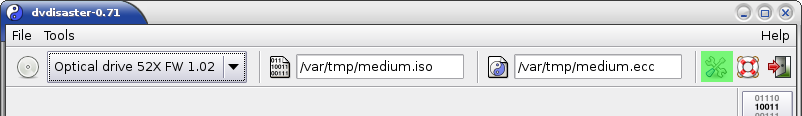
\includegraphics[width=\textwidth]{screenshots/global-prefs-invoke.png}}
\caption{Opening the configuration dialog.}  
\label{howto-scan-open-preferences}
\end{figure}

The relevant tabs are described on the next pages. They are
found in the configuration dialog.
Open the dialog by selecting the symbol marked green in the
screen shot ( \begin{minipage}{8mm}
\includegraphics{icons/prefs-icon.png}\end{minipage}, see figure \ref{howto-scan-open-preferences}).
The symbol may look different due to the symbol theme you are using.

\newpage

\begin{figure}[h]
\centerline{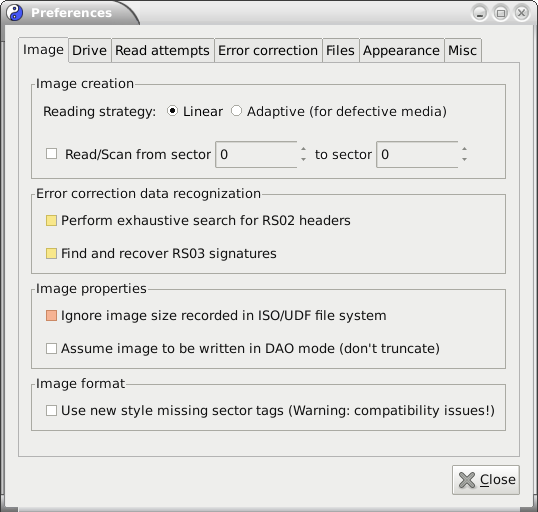
\includegraphics[width=0.9\textwidth]{screenshots/scan-prefs-image.png}}
\caption{The ``Image'' tab.}  
\label{howto-scan-prefs-image}
\end{figure}

\paragraph{Error correction data recognization.} If you
are sure that your medium contains embedded RS02 or RS03 error
correction data, activate the respective items (marked yellow).
Using the error correction (ecc) data will improve scanning results,
but searching for non existing ecc data will cost several minutes.

\paragraph{Image properties.} Selecting the proper
method for determining the image size is important.
Make sure that ``Ignore image size recorded in ISO/UDF file system''
(marked red) is switched off.
This option should only be used
in \tlnk{howto-eccfile-advanced-settings-image}{special cases during image recovery}.

\smallskip

Adjust the remaining settings as shown in the screen shot.

\newpage

\begin{figure}[h]
\centerline{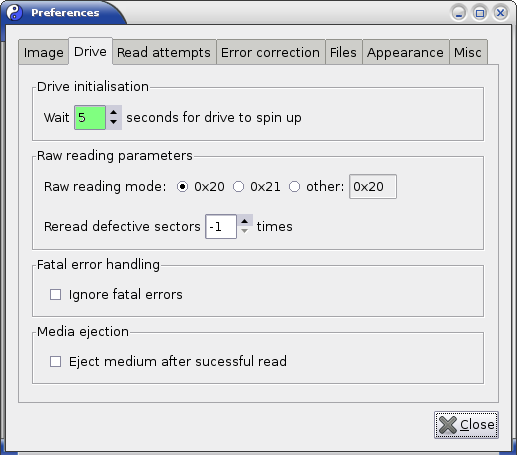
\includegraphics[width=0.9\textwidth]{screenshots/scan-prefs-drive.png}}
\caption{The ``Drive'' tab.}  
\label{howto-scan-prefs-drive}
\end{figure}

\paragraph{Drive initialization.} Reading data
from the drive while it is spinning up can generate spurious error
reports. Adjust the spin up time for your drive (typically 5-10 seconds)
in the field marked green to make dvdisaster wait for the appropriate time.

\smallskip

Leave the other settings at the values shown; you
can \tlnk{howto-scan-advanced-settings}{optimize} them later.

\newpage

\begin{figure}[h]
\centerline{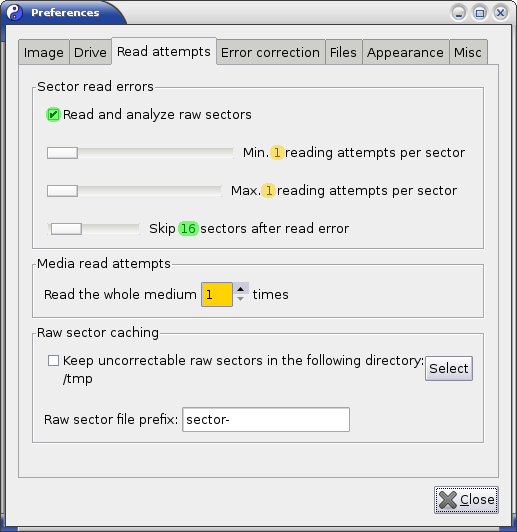
\includegraphics[width=0.9\textwidth]{screenshots/scan-prefs-read-attempts.png}}
\caption{The ``Read attempts'' tab.}  
\label{howto-scan-prefs-read-attempts}
\end{figure}

\paragraph{Sector read errors.} The option ``Read and analyse raw sectors''
(first green marking) uses C2 analysis and possibly more raw data
reported by the drive for a better assessment of CD media quality.
This setting does nothing for DVD and BD media, but it is safe to
remain activated unless it causes problems with your drive reading CDs.

Adjust the reading attempts settings as shown here. Using larger
values causes unnecessary reading activity but will not improve the scan.
After a read error no less than 16 sectors should be skipped (second
green marking); when scanning badly damaged media this setting can
be \tlnk{howto-scan-advanced-settings-read-attempts}{optimized using larger values}.

\paragraph{Media read attempts.} Performing multiple read attempts
is not recommended during a scan; set the number of retries to 1
in the three places marked in orange. Collecting raw sectors should
also be off during the scan.

\newpage

\begin{figure}[h]
\centerline{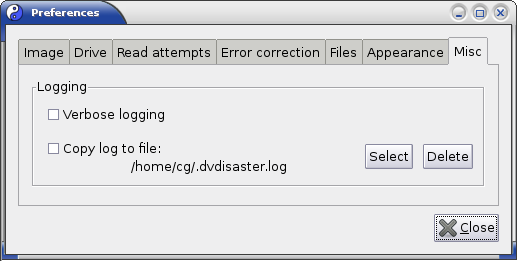
\includegraphics[width=0.9\textwidth]{screenshots/general-prefs-misc.png}}
\caption{The ``Misc'' tab.}  
\label{howto-scan-prefs-misc}
\end{figure}

\paragraph{The ``Misc Tab''.} Currently
this tab only has functions for creating log files.
This is helpful for \tlnk{reporting-defects}{reporting defects} but
should be left off during normal operation.

\paragraph{Not used tabs.} The ``Error correction'' and ``Files'' tabs
have no influence on scanning media. The ``Appearance'' tab
allows you to adapt the output colors to your taste, but these have
no further effects on the scanning process. 

\newpage
\subsubsection{Scanning for errors - Walkthrough}
\label{howto-scan-walkthrough}

Please make sure that dvdisaster has been configured as
described in the \tlnk{howto-scan-basic-settings}{basic settings} section
as some settings might negatively affect the scanning results.
Then perform the following steps: 

\bigskip

\begin{tabular}{cl}
  \begin{minipage}{50mm}
    \centerline{\slotin}
  \end{minipage}
  &
  \begin{minipage}{104mm}
  {\bf Insert the medium you want to scan into a drive} which
  is directly connected to your computer. You can not use network
  drives, software drives and drives inside virtual machines.
  \end{minipage}\\

  \begin{minipage}{50mm}
    \centerline{\downarr}
  \end{minipage}
  & \\

  \begin{minipage}{50mm}
    \centerline{\filemanager}
  \end{minipage}
  &
  \begin{minipage}{104mm}
    {\bf Close any windows} which may be opened by your
    operating system for viewing or performing the medium contents.
    Wait until the drive has recognized the medium and the medium
    has spun down. 
  \end{minipage}\\

  \begin{minipage}{50mm}
    \centerline{\downarr}
  \end{minipage}
  & \\[6mm]

  \begin{minipage}{50mm}
    \centerline{\selectdrive}
  \end{minipage}
  &
  \begin{minipage}{104mm}
    {\bf Select the drive containing the medium} in dvdisasters
    drop down menu. 
  \end{minipage}\\[4mm]

  \begin{minipage}{50mm}
    \centerline{\downarr}
  \end{minipage}
  & \\

  \begin{minipage}{50mm}
    \centerline{\selectecc}
  \end{minipage}
  &
  \begin{minipage}{104mm}
    {\bf Select the error correction file for this medium} if you
    have one available. Ecc data from RS02 or RS03 augmented media
    is used automatically.
  \end{minipage}\\

  \begin{minipage}{50mm}
    \centerline{\downarr}
  \end{minipage}
  & \\[6mm]

  \begin{minipage}{50mm}
    \centerline{\scanicon}
  \end{minipage}
  &
  \begin{minipage}{104mm}
    Start the scan by {\bf clicking the "Scan" button.}
  \end{minipage}\\[6mm]

  \begin{minipage}{50mm}
    \centerline{\downarr}
  \end{minipage}
  & \\[6mm]

  \begin{minipage}{50mm}
    \centerline{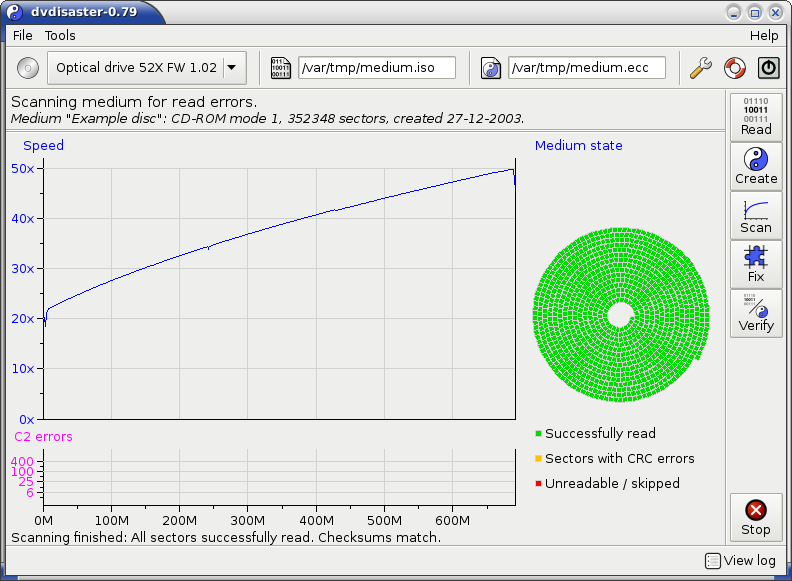
\includegraphics[width=40mm]{screenshots/good-cd-scan.png}}
  \end{minipage}
  &
  \begin{minipage}{104mm}
    {\bf Watch the scanning progress.} Do not perform any other
    actions on your computer while the scan is running.
    Opening or working with other programs as well as moving
    other windows around might affect the scanning results. 
  \end{minipage}\\
\end{tabular}

\newpage
\subsubsection{Interpreting the results}
\label{howto-scan-interpret}

\begin{figure}[h]
\centerline{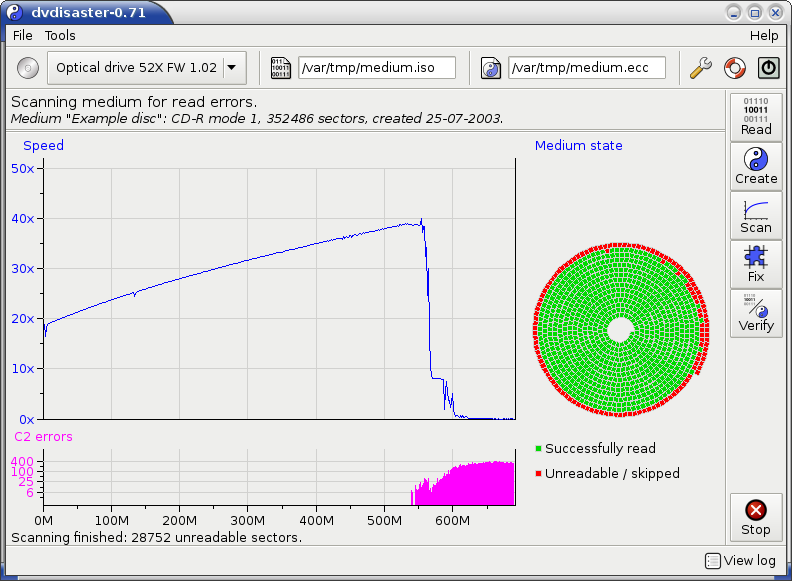
\includegraphics[width=0.97\textwidth]{screenshots/defective-cd-scan.png}}
\caption{Scanning the medium.}  
\label{howto-scan-general-results}
\end{figure}

\vspace*{-5mm}

\paragraph{Overview.} dvdisaster provides several information
about the scanning results (see fig. \ref{howto-scan-general-results}): 

\begin{itemize}
  \item The spiral under {\bf ``Medium State''} (to the right).

    The spiral provides information about the medium readability.
    The medium is fully readable when all segments of the spiral
    are colored green. Yellow or red blocks mark places where data
    could not be correctly read from the medium. The total number
    of unreadable sectors is printed in the ``Scanning finished:''
    message at the window bottom.

  \item {\bf ``Speed''} - The reading speed curve (upper left).

    The reading speed is not an absolute gauge of the medium
    health, but it is usable as a rule of thumb: The more
    regular the curve, the better the medium. You will
    find examples of good and bad reading speed curves on the following pages.

  \item {\bf ``C2 errors''} - A medium state gauge provided by the drive (down left).

    This kind of analysis is \tlnk{qa-quality-scans}{currently only available for CD media}.
    CD drives have a built-in error correction
    which can eliminate small data losses caused by minor
    defects on the medium. The number of C2 errors is a
    measurement of how often the drive needed to employ its
    internal error correction during the read - this value
    should be zero on good media.
\end{itemize}

\newpage
\begin{figure}[h]
\centerline{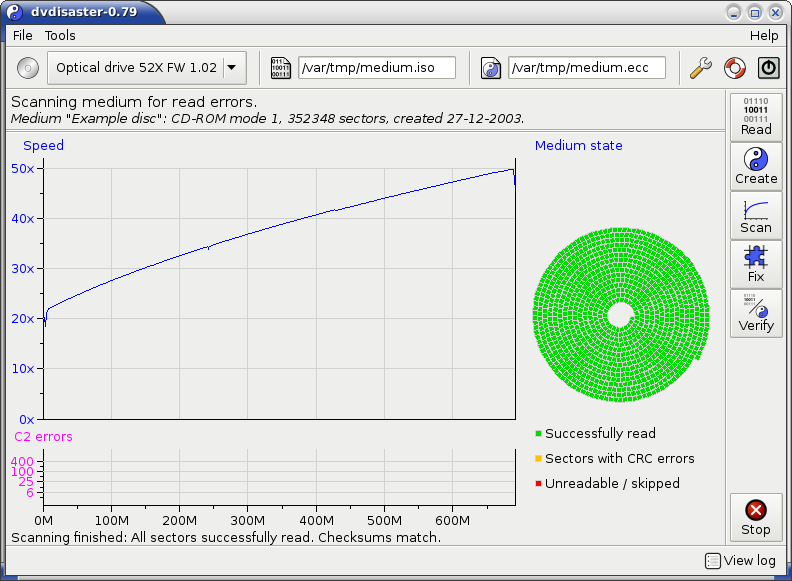
\includegraphics[width=\textwidth]{screenshots/good-cd-scan.png}}
\caption{Good CD.}  
\label{howto-scan-good-cd}
\end{figure}

{\bf Example of a good medium:} This screen shot shows
a perfect CD: All blocks under ``Medium state'' are green, no C2
errors have been reported and the reading curve runs smoothly.
A rising reading speed is normal for most media (see the next screen
shot for a counter example). The small spikes at the beginning and
at the end of the curve are normal; minor glitches like the one shown
at 250M are also harmless.

\newpage
\begin{figure}[h]
\centerline{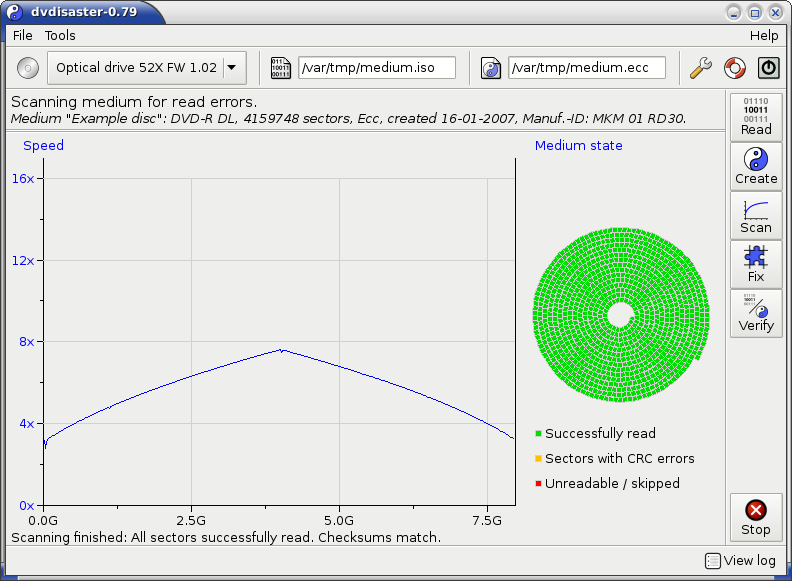
\includegraphics[width=\textwidth]{screenshots/good-dvd9-scan.png}}
\caption{Good two-layered DVD.}  
\label{howto-scan-good-two-layered-dvd}
\end{figure}

{\bf Sometimes the reading curve won't rise steadily:} Multi-layered
media might yield reading curves which are rising and dropping
in a symmetric pattern. Not shown but also possible are flat
curves without any change in reading speed (most typically seen
with DVD-RAM).

\newpage
\begin{figure}[h]
\centerline{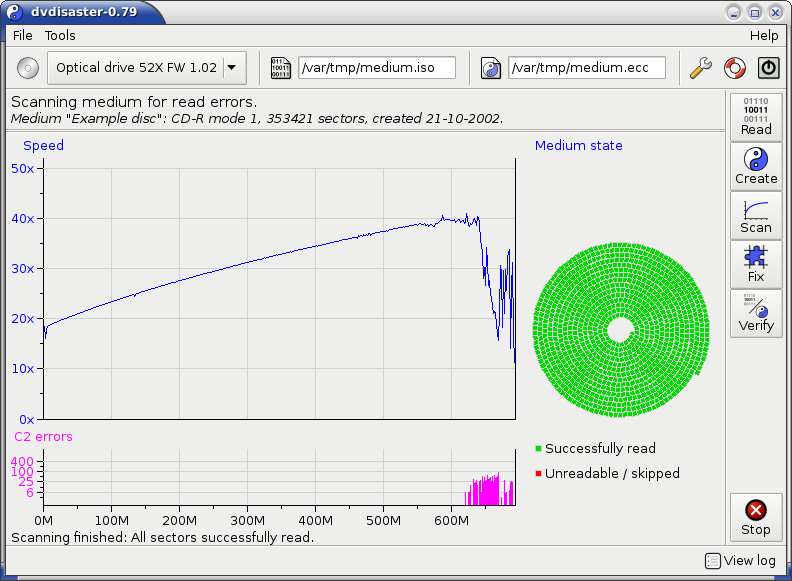
\includegraphics[width=\textwidth]{screenshots/weak-cd-scan.png}}
\caption{Weak CD.}  
\label{howto-scan-weak-cd}
\end{figure}

{\bf An example of a weak medium.} This medium is still
readable as indicated by the green spiral shown under ``Medium state''.
However there are clear signs of serious trouble ahead: The drive must
slow down significantly towards the end of the medium in order to read
from it. Note the steep fall of reading speed after the 600M mark.
This comes along with C2 error rates rising to the 100 mark; this is
another warning that the medium is decaying in the outer region.
If you have not created \tlnk{howto-ecc}{error correction data} this is probably the
last opportunity to do so as the medium will develop the first
read errors soon.

\newpage
\begin{figure}[h]
\centerline{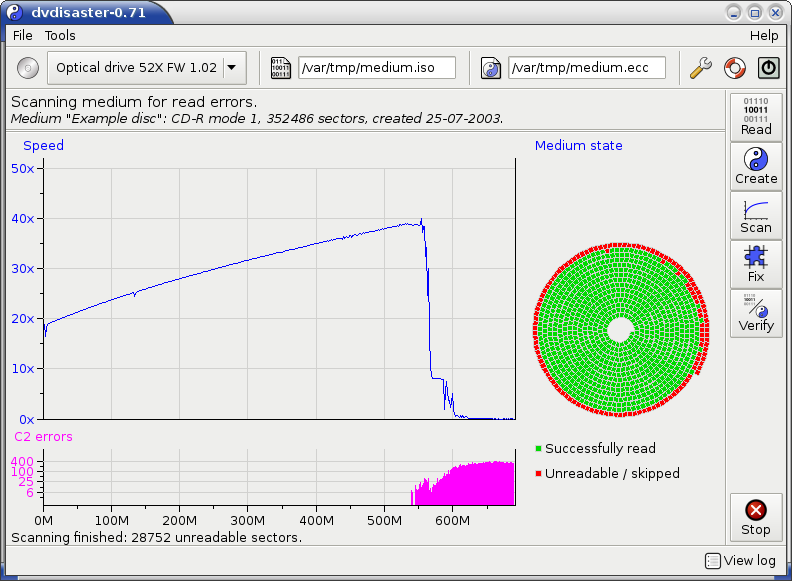
\includegraphics[width=\textwidth]{screenshots/defective-cd-scan.png}}
\caption{Defective CD.}  
\label{howto-scan-defective-cd}
\end{figure}

{\bf Example of a defective CD.} \label{howto-interpret-defective-cd}
The red sectors in the spiral
visualize large unreadable sections in the outer region of the medium.
At the bottom of the window you will find the information that the
medium contains 28752 unreadable sectors. This sums up to about
8.2\% defective sectors (of 352486 sectors total) and is well within
the \tlnk{howto-recover}{recovery} bounds
by \tlnk{howto-ecc}{error correction (ecc) data} made with default
settings - if you have made the ecc data in time! Otherwise the
contents of the red sectors are lost since ecc data cannot be
created from already defective media.

\newpage
\begin{figure}[h]
\centerline{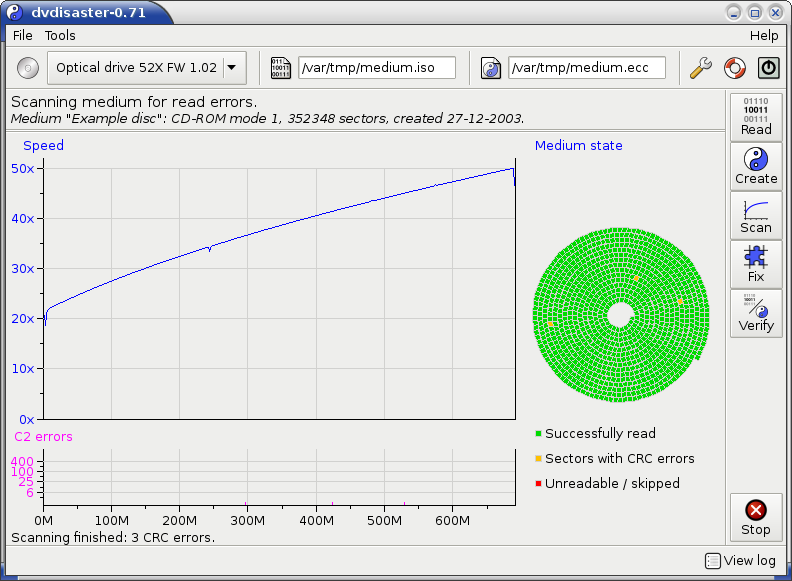
\includegraphics[width=\textwidth]{screenshots/crc-cd-scan.png}}
\caption{Checksum errors.}  
\label{howto-scan-checksum-errors}
\end{figure}

{\bf Checksum errors.} Yellow spots in the spiral depict places
where the medium was fully readable, but the data read did not
match checksums in the error correction data. There are two main causes:

\begin{itemize}
\item The image has been manipulated after the creation of
  error correction data and before writing it to the medium.
  This can happen when the image is mounted with
  write access after ecc data has been created. Typical signs are
  CRC errors in sector 64 and in sectors 200 to 400 as the system
  updates the file access times there. Performing a data recovery
  using dvdisaster is typically harmless in this situation.

  \medskip

  However if you have modified files in the image after
  creating the ecc data, the error correction data will be both
  worthless and dangerous. Applying a recovery to the medium will
  restore the image state at the time the ecc data has been created,
  and this will obviously not represent the most recent contents of
  the medium.

\item There are technical problems with the computer system,
  especially in mass storage communication. Perform the scan again
  and observe the CRC error locations. If CRC errors disappear
  or surface at different locations your system might have
  defective RAM, bad drive cabling/controllers or incorrect clock speeds.
\end{itemize}

\newpage
\subsubsection{Advanced settings}
\label{howto-scan-advanced-settings}

\begin{figure}[h]
\centerline{\includegraphics[width=0.9\textwidth]{screenshots/scan-prefs-drive-adv.png}}
\caption{Advanced settings in the ``Drive'' tab.}  
\label{howto-scan-prefs-drive-adv}
\end{figure}

{\bf Fatal error handling.} dvdisaster will normally abort the scan
when the drive reports a fatal internal error like mechanical problems.
The intention is to avoid damaging the drive. However some drives
will erroneously report such problems when they get confused by
damaged media. If you have such a drive you can use this option
to force the scan to continue.

\bigskip

{\bf Media ejection.} dvdisaster tries to eject the medium after
a successful scan if this option is activated. However ejecting
the medium might be prohibited by the operating system so this
is not guaranteed to work. For example if upon media insertion
a window is opened for performing the contents it may not be
possible to automatically eject the medium.

\newpage
\begin{figure}[h]
\centerline{\includegraphics[width=0.9\textwidth]{screenshots/scan-prefs-read-attempts-adv.png}}
\caption{Advanced settings in the ``Read attempts'' tab.}  
\label{howto-scan-prefs-read-attempts-adv}
\end{figure}

{\bf Sector read errors.} \label{howto-scan-advanced-settings-read-attempts} Attempts
for reading defective sectors
cost a lot of time. Since it is likely to encounter another defective
sector after hitting a read error, skipping a few sectors after a
read error saves time and reduces wear on the drive. If you only want
a quick overview of a damaged medium setting this value to 1024 might help.
But keep in mind that all skipped sectors are counted as being defective
so the number of reported errors becomes higher and less accurate.

\newpage
\subsection{Selecting the right type of ecc data}
\label{howto-ecc}

Error correction data can either be created in form of
a separate error correction file or it can be placed directly
onto the medium.

\smallskip

Answering the following questions can quickly guide you to the right
ecc data format:

\begin{itemize}
\item {\em Do you need error correction data for a medium which has already been written?}

  In that case, you need to \tlnk{howto-eccfile}{create an error
    correction file} because an already existing medium can not be
  augmented with error correction data. 

\item {\em Are you planning to write the medium right now?}

  If the medium is full or nearly full (less than 20\% free),
  not enough space might be available for storing the error
  correction data. It is strongly recommended to \tlnk{howto-eccfile}{create an
  error correction file} in that case. Otherwise, you can put
  the \tlnk{howto-augment}{error correction data directly onto the medium}.
  To do so you must create an ISO image first and then augment it with
  error correction data before you write it to the medium. 
\end{itemize}

\paragraph{More information on keeping error correction data.}\quad

dvdisaster helps protecting your media from data loss by
forehanded\footnote{ Let's repeat again for clarity: Error correction data
  must be created before the medium becomes defective. It is not possible
  to create error correction data from defective media; in that case
  unreadable sectors can not be recovered.} creation of error correction
data. Error correction data must be treated like normal backup data,
e.g. you need to keep it available during the whole lifetime of the
respective medium.

\smallskip

The easiest way is storing the error correction data on the medium
you want to protect. But this is only possible if the medium has not
yet been written: To employ this method you need to create an ISO image
first, then augment this image with error correction data, and finally
write the augmented image to the medium.

\smallskip

If the medium has already been written, or insufficient space is left
for augmenting the image, you still can create error correction data
in form of a free-standing error correction file. This file must then
be stored somewhere else, e.g. you need to take additional provisions
to \tlnk{howto-eccfile-archival}{archive your error correction files}.

\smallskip

More information about the pro and con of these methods can be found
in the \tlnk{background-methods}{background information} section. 

\newpage

\subsection{Creating ecc data as a separate file}
\label{howto-eccfile}

\begin{tabular}{ll}
  {\bf Task} & An error correction file is created for an optical medium. \\

  &
  \begin{minipage}{132mm}

    \bigskip

    Note: This page describes how error correction data is created
    and placed into a separate file. There is also a method for
    placing the error correction data \tlnk{howto-augment}{directly onto the medium}.

    \smallskip
    
    \tlnk{howto-ecc}{Would you like help on deciding between these two methods?}
    \end{minipage}\\[15mm]
    
  {\bf Required:} & \\[3mm]

  \begin{minipage}{15mm}
    \goodcd
  \end{minipage} &
  \begin{minipage}{132mm}
    A good, error free\footnotemark medium,
  \end{minipage} \\

  & or \\

  \begin{minipage}{15mm}
    \goodimage
  \end{minipage} &
  \begin{minipage}{132mm}
    \addtocounter{footnote}{-1}
    an already existing and complete\footnotemark ISO
    image of the medium (e.g. the image used for
    writing the medium). 
  \end{minipage} \\[10mm]

  {\bf What to do:} &
  \tlnk{howto-eccfile-basic-settings}{1. Configure basic settings} \\[2mm]

  &
  \tlnk{howto-eccfile-create}{2. Create the error correction file} \\[2mm]

  &
  \tlnk{howto-eccfile-archival}{3. Archive the error correction file}
\end{tabular}

\footnotetext{Error correction data must be
      created before any data loss occurs: It is not possible
      to create error correction files from an already defective
      medium.}

\vspace{10mm}

\subsubsection{Basic settings for reading the image from the medium}
\label{howto-eccfile-basic-settings}
\label{howto-eccfile-basic-settings-reading}

\begin{figure}[h]
\centerline{\includegraphics[width=\textwidth]{screenshots/global-prefs-invoke.png}}
\caption{Opening the configuration dialog.}  
\label{howto-eccfile-open-preferences-eccfile}
\end{figure}

The relevant tabs are described on the next pages. They are
found in the configuration dialog.
Open the dialog by selecting the symbol marked green in the
screen shot ( \begin{minipage}{8mm}\includegraphics{icons/prefs-icon.png}\end{minipage}, see figure \ref{howto-eccfile-open-preferences-eccfile}).
The symbol may look different due to the symbol theme you are using.

\bigskip

\begin{tabular}{cl}
  \begin{minipage}{20mm}
    \centerline{\goodimage}
  \end{minipage} &
  \begin{minipage}{133mm}
      If you already have an ISO image available you can skip the next
      three tabs and proceed with
      the \tlnk{howto-eccfile-basic-settings-ecc}{error correction settings}.
      But make sure that you really have an ISO type image; other formats
      like ``.nrg'' do not produce usable error correction data.
    \end{minipage}\\
 \end{tabular}
    
\newpage

\begin{figure}[h]
\centerline{\includegraphics[width=0.9\textwidth]{screenshots/eccfile-prefs-image.png}}
\caption{The ``Image'' tab.}  
\label{howto-eccfile-prefs-image}
\end{figure}

\paragraph{Reading strategy.} Make sure that the linear reading strategy is selected
(marked green).

\bigskip

All other options should be turned off; especially those marked green as they
might have adverse effects on the image reading process. 

\newpage

\begin{figure}[h]
\centerline{\includegraphics[width=0.9\textwidth]{screenshots/eccfile-prefs-drive.png}}
\caption{The ``Drive'' tab.}  
\label{howto-eccfile-prefs-drive}
\end{figure}

\paragraph{Drive initialization.} Reading data from the drive while it is spinning
up can generate spurious error reports. Adjust the spin up time for your
drive (typically 5-10 seconds) in the field marked green to make dvdisaster
wait for the appropriate time.

\bigskip

Leave the other settings at the shown values.

\newpage

\begin{figure}[h]
\centerline{\includegraphics[width=0.9\textwidth]{screenshots/eccfile-prefs-read-attempts.png}}
\caption{The ``Read attempts'' tab.}  
\label{howto-eccfile-prefs-read-attempts}
\end{figure}

\paragraph{Sector read errors.} The option ``Read and analyze raw sectors'' (marked green)
uses additional information provided by the drive to check the integrity of read data.
This is recommended as we are interested in creating error correction data
from a properly read image.

\medskip

On the other hand since error correction data can only be created from fully
readable media we do not need multiple reading attempts and caching of
raw sectors as shown in the screen shot. 

\newpage
\subsubsection{Basic settings for the error correction data}
\label{howto-eccfile-basic-settings-ecc}

\begin{figure}[h]
\centerline{\includegraphics[width=0.9\textwidth]{screenshots/eccfile-prefs-ecc-file3.png}}
\caption{The ``Error correction'' tab for the RS03 codec.}  
\label{howto-eccfile-prefs-ecc-file3}
\end{figure}

Error correction files can be created using either the RS03 or the RS01 method
(see this \tlnk{background-methods}{comparison} for details).
It is recommended to use RS03 as it contains all features present in RS01,
but encodes much faster due to certain optimizations.

\paragraph{Settings for encoding with the RS03 method.} First select the entry
``Multithreaded RS codec (RS03)'' in the drop down menu (marked green).
After this selection the contents of the tab will display the choices given
for the RS03 method. 

\paragraph{Error correction storage.} Select ``File'' (also marked green).
This option causes error correction data to be stored in a separate file
and will also make the redundancy choice available which is located below.

\paragraph{Redundancy for new error correction files.} Select the redundancy
which suits your needs. The redundancy will determine the maximum error
correction capability: An error correction file with x\% redundancy can
correct up to x\% of read errors under optimal circumstances.
Since the best case is usually not encountered you should add some safety
margin to the redundancy by picking one of the following choices (see yellow markings):

\begin{itemize}
\item The ``normal'' and ``high'' presets provide a redundancy of 14.3\% and 33.5\%
  respectively.
\item You can freely choose the redundancy by activating the ``other'' item
  and dragging the slider.
\item By activating the ``Use at most'' button you can specify the error
  correction file size in MiB. dvdisaster will choose a suitable redundancy
  so that the error correction file will be close to but not larger than the
  specified size.
\end{itemize}
  
The redundancy will also determine the size of the error correction file;
using x\% redundancy will create an error correction file of about x\% the
size of the image. Using redundancies lower than the ``normal'' setting (14.3\%)
is not recommended as the error correction might be overloaded too quickly.

\paragraph{Multithreading.} The RS03 encoder can distribute its workload
onto multiple processor cores by using multithreading. On machines with
up to four cores, set the number of threads equal to the number of
cores (e.g. use 4 threads on a 4 core machine). On machines with more
than 4 cores, use one thread less than the number of available cores;
e.g. use 7 threads on an 8 core machine - this leaves one core free
for housekeeping tasks).

\smallskip

Leave the other settings as shown in the screenshot; you can
\tlnk{howto-eccfile-advanced-settings-ecc}{optimize} them later.

\newpage

\begin{figure}[h]
\centerline{\includegraphics[width=0.9\textwidth]{screenshots/eccfile-prefs-ecc-file1.png}}
\caption{The ``Error correction'' tab for the old RS01 codec.}  
\label{howto-eccfile-prefs-ecc-file1}
\end{figure}

\paragraph{Settings for encoding with the RS01 method.} If you want to
use the old RS01 method, choose ``Error correction file (RS01)'' in
the ``Storage method'' drop down menu (green marking; see
fig. \ref{howto-eccfile-prefs-ecc-file1}).

\smallskip

Then select a redundancy setting which suits your needs; see the
explanations on redundancy for the RS03 method above for more information.
For RS01, the ``normal'' and ``high'' settings are somehow optimized for
speed, but still much slower than their RS03 counterparts. 

\newpage

\begin{figure}
\centerline{\includegraphics[width=0.9\textwidth]{screenshots/create-prefs-file.png}}
\caption{The ``Files'' tab.}  
\label{howto-eccfile-prefs-file}
\end{figure}

\paragraph{The ``Files'' tab.} In this tab, only
activate the option for confirming file overwriting.
Leave the other options off for the moment; suggestions for
further \tlnk{howto-eccfile-advanced-settings}{optimization} follow later. 

\bigskip

\paragraph{Not used tabs.} The ``Misc'' tab currently has only functions
for creating log files. This is helpful
for \tlnk{reporting-defects}{reporting defects} but
should be left off during normal operation. The ``Appearance'' tab allows
you to adapt the output colors to your taste, but these have no further
effects on the error correction data creation.

\newpage
\subsubsection{Creating the error correction file}
\label{howto-eccfile-create}

\begin{tabular}{cccl}
  \begin{minipage}{15mm}
    \goodcd
  \end{minipage}
  &
  \begin{minipage}{10mm}
    \rightarr
  \end{minipage}
  &
  \begin{minipage}{15mm}
    \goodimage
  \end{minipage}
  &
  \begin{minipage}{105mm}
    The error correction file can only be created from an ISO image
    on hard disk, not directly from the medium. If you have the
    ISO image already/still available from making the medium,
    turn over to the next page. Otherwise, follow these instructions
    for extracting the ISO image from the medium.
  \end{minipage}
  \\
\end{tabular}

\bigskip

\hrulefill

\bigskip

\begin{tabular}{cl}
  \begin{minipage}{50mm}
    \centerline{\slotin}
  \end{minipage}
  &
  \begin{minipage}{104mm}
  {\bf Insert the medium you want to read into a drive} which
  is directly connected to your computer. You can not use network
  drives, software drives and drives inside virtual machines.
  \end{minipage}\\

  \begin{minipage}{50mm}
    \centerline{\downarr}
  \end{minipage}
  & \\

  \begin{minipage}{50mm}
    \centerline{\filemanager}
  \end{minipage}
  &
  \begin{minipage}{104mm}
    {\bf Close any windows} which may be opened by your
    operating system for viewing or performing the medium contents.
    Wait until the drive has recognized the medium and the medium
    has spun down. 
  \end{minipage}\\

  \begin{minipage}{50mm}
    \centerline{\downarr}
  \end{minipage}
  & \\[6mm]

  \begin{minipage}{50mm}
    \centerline{\selectdrive}
  \end{minipage}
  &
  \begin{minipage}{104mm}
    {\bf Select the drive containing the medium} in dvdisasters
    drop down menu. 
  \end{minipage}\\[4mm]

  \begin{minipage}{50mm}
    \centerline{\downarr}
  \end{minipage}
  & \\

  \begin{minipage}{50mm}
    \centerline{\selectimage}
  \end{minipage}
  &
  \begin{minipage}{104mm}
    {\bf Select a directory and file name} for
    storing the ISO image.
  \end{minipage}\\[4mm]

  \begin{minipage}{50mm}
    \centerline{\downarr}
  \end{minipage}
  & \\

  \begin{minipage}{50mm}
    \centerline{\readicon}
  \end{minipage}
  &
  \begin{minipage}{104mm}
    {\bf Create the ISO image} by clicking the "Read" button.
  \end{minipage}\\[6mm]

  \begin{minipage}{50mm}
    \centerline{\downarr}
  \end{minipage}
  & \\[6mm]

  \begin{minipage}{50mm}
    \centerline{\includegraphics[width=40mm]{screenshots/good-cd-scan.png}}
  \end{minipage}
  &
  \begin{minipage}{104mm}
    {\bf Watch the reading progress.}
    Wait until the medium has been completely read.
    If the medium turns out to contain defective sectors
    it will not be possible to create error correction data. 
  \end{minipage}\\
\end{tabular}

\bigskip
  
Now continue with the next page to create an error correction file
from the ISO image.

\newpage
\label{howto-eccfile-create-ecc}

\begin{tabular}{cccl}
  \begin{minipage}{15mm}
    \goodimage
  \end{minipage}
  &
  \begin{minipage}{10mm}
    \rightarr
  \end{minipage}
  &
  \begin{minipage}{15mm}
    \eccfile
  \end{minipage}
  &
  \begin{minipage}{105mm}
    Now that we have an ISO image of the medium, we can create the
    error correction file from it. It you do not have the ISO image yet,
    please follow the instructions on the previous page for
    extracting it from the medium.
  \end{minipage}
  \\
\end{tabular}

\bigskip

\hrulefill

\bigskip

\begin{tabular}{cl}
  \begin{minipage}{50mm}
    \centerline{\selectimage}
  \end{minipage}
  &
  \begin{minipage}{104mm}
    {\bf Select the directory and name of the ISO image} for which you want 
    to create the error correction data. It is assumed that the ISO image 
    has been created by some other means, e.g. by using your optical disc 
    authoring software. If you extracted the ISO image from a medium using
    dvdisaster as described one page before, this field is already filled in
    correctly.
  \end{minipage}\\[-8mm]

  \begin{minipage}{50mm}
    \centerline{\downarr}
  \end{minipage}
  & \\[5mm]

  \begin{minipage}{50mm}
    \centerline{\selectecc}
  \end{minipage}
  &
  \begin{minipage}{104mm}
    {\bf Select a directory and name} for storing the error correction file.
  \end{minipage}\\[4mm]

  \begin{minipage}{50mm}
    \centerline{\downarr}
  \end{minipage}
  & \\[6mm]

  \begin{minipage}{50mm}
    \centerline{\createicon}
  \end{minipage}
  &
  \begin{minipage}{104mm}
    {\bf Create the error correction file} by clicking the "Create" button.
  \end{minipage}\\[6mm]

  \begin{minipage}{50mm}
    \centerline{\downarr}
  \end{minipage}
  & \\[6mm]

  \begin{minipage}{50mm}
    \centerline{\includegraphics[width=40mm]{screenshots/watch-create.png}}
  \end{minipage}
  &
  \begin{minipage}{104mm}
    {\bf Wait until the creation process finishes.} This 
    may take a while depending on the image size, selected redundancy 
    and used encoding method.
  \end{minipage}\\[14mm]

  \begin{minipage}{50mm}
    \centerline{\downforkarr}
  \end{minipage}
  & \\[6mm]

  \begin{minipage}{24mm}
    \centerline{\oldimage}
  \end{minipage}
  \begin{minipage}{24mm}
    \centerline{\eccfile}
  \end{minipage}
  &
  \begin{minipage}{104mm}
    {\bf Wrapping up.} You can delete the image file now. However 
    you must keep the error correction file and, even more important, 
    protect it from being damaged. Refer to the next page for some 
    suggestions about \tlnk{howto-eccfile-archival}{error correction file archival}. 
  \end{minipage}\\
\end{tabular}

\newpage
\subsubsection{Tips for archival of error correction files}
\label{howto-eccfile-archival}

Optical discs are currently among the most cost-effective exchangeable
mass storage media. Therefore you are probably considering them for
storing error correction files.

\medskip

Nothing is wrong with doing so, but be aware that your data and protective
error correction files are kept on media with equal reliability.
When you encounter read errors on a data medium it is likely that
the medium containing the respective error correction files has also
gone defective. After all both media have been written at the same time,
and they have the same aging characteristics.

\medskip

This might come at a surprise, but it can not be
guaranteed that an error correction file remains usable
when it is stored on a defective medium - here
is a \tlnk{background-image-level}{explanation of the technical background}.\marginpar{\hfill\rule{1mm}{13mm}} 

\medskip

Therefore it is important to protect error correction files just as
if they were normal data. To be more specific, the medium containing
error correction files must be protected with error correction data as well.
Here are two ways of doing this:

\begin{enumerate}
\item Storing error correction files on separate media:

Use additional media just for keeping the error correction files.
If you use no more than 80\% per medium for error correction files
it can be \tlnk{howto-augment}{augmented with error correction data}.
This allows you to recover the medium if you run into problems reading
the error correction files at a later time.

\item Storing error correction files on the next medium in sequence:

Maybe you are using media for an incremental backup strategy.
In that case you could collect files until the first medium can be filled.
Write that medium as usual and create an error correction file for it.
Include that error correction file into the backup set which will go onto
the second medium. When the second medium has been written, write the error
correction file for it onto the third medium and so on. This way all media
in the chain are protected with error correction files (with the ecc file
for the last medium residing on hard disk until another medium is written).
\end{enumerate}

Of course Murphys Law may strike and result in all media of the chain
becoming defective. In that case you need to recover all media, starting
with the most recent one ;-)

\newpage
\subsubsection{Advanced settings for the error correction data}
\label{howto-eccfile-advanced-settings}
\label{howto-eccfile-advanced-settings-image}

\vspace{-4mm}
\begin{figure}[h]
\centerline{\includegraphics[width=0.9\textwidth]{screenshots/eccfile-prefs-image-adv.png}}
\caption{The ``Image'' tab.}  
\label{howto-eccfile-prefs-image-adv}
\end{figure}
\vspace{-6mm}

\paragraph{Error correction data recognization.} Since
we are reading the image for the purpose of creating error correction data, it
makes no sense to look for error correction data in the image itself and the options
marked green should remain turned off.

\paragraph{Image properties.} In some cases it might be necessary to change to way
dvdisaster determines the size of the ISO image. The normal strategy is to
query the ISO image from the ISO/UDF file system, and only if this fails,
to query the information directly from the optical drive. Using this order makes
sense as image sizes reported by most drives are unreliable in many cases while
ISO/UDF file system information is usually correct. However in some rare cases the
image size recorded in the ISO/UDF filesystem is wrong. Some GNU/Linux live CDs may have
this problem. If you read back the ISO image from such CDs and its md5sum does not
match the advertised one from the download site, try re-reading the image with
the ``Ignore image size recorded in ISO/UDF file system'' option (marked red)
turned on. But do not blindly turn this option on as it could
create sub optimal or corrupted ISO images, especially if you plan to use the
image for error correction data generation. 

\newpage

\begin{figure}[h]
\centerline{\includegraphics[width=0.9\textwidth]{screenshots/eccfile-prefs-drive-adv.png}}
\caption{The ``Drive'' tab.}  
\label{howto-eccfile-prefs-drive-adv}
\end{figure}

\paragraph{Media ejection.} This feature is helpful
when you are processing a batch of media. Use it together with the
options shown in the ``Files tab'' at the next page.

\smallskip

dvdisaster will try to eject the medium after the image has
been read. However ejecting the medium might be prohibited by
the operating system so this is not guaranteed to work. For example if upon
media insertion a window is opened for performing the contents it may not be possible to
automatically eject the medium.

\newpage

\begin{figure}[h]
\centerline{\includegraphics[width=0.9\textwidth]{screenshots/eccfile-prefs-file-adv.png}}
\caption{The ``Files'' tab.}  
\label{howto-eccfile-prefs-file-adv}
\end{figure}

\paragraph{Local files (on hard disk).} To ease entering new file names,
activate the option marked yellow.
This will append the ``.iso'' and ``.ecc'' file name extensions automatically.

\paragraph{Automatic file creation and deletion.} You can automate the
process of creating error correction files using these options. The
first option marked green lets dvdisaster create the error correction
file immediately after the medium has been (completely) read.
The second option marked green deletes the image when the error correction
file has been successfully created.

\bigskip

\paragraph{Please note:} Remember to choose a different name for the error
correction file after inserting a new medium. Otherwise the
previous error correction file will be overwritten. 

\newpage

\begin{figure}[h]
\centerline{\includegraphics[width=0.9\textwidth]{screenshots/eccfile-prefs-ecc3-adv.png}}
\caption{The ``Error correction'' tab for the RS03 codec.}  
\label{howto-eccfile-prefs-ecc3-image-adv}
\end{figure}

\paragraph{Optimizing the error correction data creation.}\quad
\label{howto-eccfile-advanced-settings-ecc}

Creating error correction data requires both huge processing power
and high random access disk I/O capabilities. When encoding on conventional
hard disks with spinning platters, disk I/O will be the limiting
factor over all other hardware. Therefore it is recommended to encode on
fast storage media like SSDs, or even better, on RAM-based filesystems such
as /dev/shm on GNU/Linux.

\paragraph{I/O parameters.} dvdisaster optimizes access to the
image and error correction data by preloading and caching parts of them.
The optimal preload value (marked red) depends on the storage system
used for the image and error correction files. Use small preload values
for systems with low latency and seek time, e.g. SSDs and the RAM file system.
For magnetic hard disks performance may be better using larger preload values.
Make sure that you do not use more than half of your physical RAM for preloading.
A preload value of $n$ will use approx. $n$ MiB of RAM.

\medskip

The I/O strategy option (marked green) controls how dvdisaster performs
its disk I/O while creating error correction data. Try both options and
see which performs best on your hardware.

The read/write option activates dvdisaster's own I/O scheduler which
reads and writes image data using normal file I/O. The advantage of this
scheme is that dvdisaster knows exactly which data needs to be cached and preloaded;
the disadvantage is that all data needs to be copied between the kernel and
dvdisaster's own buffers. Usually, this I/O scheme works best on slow
storage with high latency and seek times; e.g. on all storage involving spinning platters.

The memory mapped option uses the kernel's memory mapping scheme for direct access
to the image file. This has the advantage of minimal overhead, but may be
adversely affected by poor caching and preloading decisions made by the kernel
(since the kernel does not know what dvdisaster is going to do with the data).
This scheme performs well when encoding in a RAM-based file system
(such as /dev/shm on GNU/Linux) and on very fast media with low latency such as SSDs.

\paragraph{Multithreading.} RS03 can use multiple threads - and
therefore CPU cores - for encoding (yellow slider). For systems with 4 cores
or less, start with setting the number of threads to the number of cores.
If you have more cores, leave one core for doing I/O and graphics updates,
e.g. use 7 threads on an 8 core system. On systems with hyper-threading
capabilities, increasing the number of threads until double the number
of physical cores might improve performance.

\smallskip

Do not expect performance to scale linearly with the number of used
CPU cores (although it should do so for at least the first four to
eight cores). Hard disk performance is more limiting than raw CPU power.
When using more than 8 cores, memory bandwidth may eventually limit performance.

\paragraph{Encoding algorithm.} This option affects the speed of
generating RS03 error correction data per CPU core (buttons marked blue).
dvdisaster can either use a generic encoding algorithm using 32bit or 64bit
wide operations running on the integer unit of the processor,
or use processor specific extensions.
Available extensions are SSE2 for x86 based processors and AltiVec on
PowerPC processors. These extensions encode with 128bit wide operations
and will usually provide the fastest encoding variant.
If ``auto'' is specified, the SSE2/AltiVec algorithms will be selected
if the processor supports them. 

\newpage

\subsection{Putting error correction data directly onto the medium}
\label{howto-augment}

\begin{tabular}{ll}
  {\bf Task} & Error correction data is stored along with the user data on the same medium. \\

  &
  \begin{minipage}{132mm}

    \bigskip

    Note: This page describes how an ISO image is augmented with error
    correction data prior to writing it onto a medium.
    There is also a method for creating and placing error correction data
    \tlnk{howto-eccfile}{into a separate file}. 

    \smallskip
    
    \tlnk{howto-ecc}{Would you like help on deciding between these two methods?}
    \end{minipage}\\[15mm]
    
  {\bf Required:} & \\[-5mm]

  \begin{minipage}{15mm}
\vspace*{8mm}
    \goodimage
  \end{minipage} &
  \begin{minipage}{132mm}
    \begin{itemize}
      \item an authoring (``burning'') software capable of creating ISO images
      \item the medium which is to be augmented with error correction data has not yet
        been written (already written media can not be augmented)
      \item at least 20\% of free space on the medium which is to be created
    \end{itemize}
  \end{minipage} \\[15mm]


  {\bf What to do:} &
  \tlnk{howto-augment-basic-settings}{1. Configure basic settings} \\[2mm]

  &
  \tlnk{howto-augment-make-iso}{2a. Create an ISO image,} \\[2mm]

  &
  \tlnk{howto-augment-overview-ecc}{2b. augment it with error correction data,} \\[2mm]

  &
  \tlnk{howto-augment-write-iso}{2c. and write it to a medium.} \\[2mm]

\end{tabular}

%\footnotetext{An already written medium can not be augmented with error correction data.}

%\vspace{10mm}

\subsubsection{Basic settings for augmenting images with ecc data}
\label{howto-augment-basic-settings}

\begin{figure}[h]
\centerline{\includegraphics[width=\textwidth]{screenshots/global-prefs-invoke.png}}
\caption{Opening the configuration dialog.}  
\label{howto-eccfile-open-preferences-augment}
\end{figure}

The relevant tabs are described on the next pages. They are
found in the configuration dialog.
Open the dialog by selecting the symbol marked green in the
screen shot ( \begin{minipage}{8mm}\includegraphics{icons/prefs-icon.png}\end{minipage}, see figure \ref{howto-eccfile-open-preferences-augment}).
The symbol may look different due to the symbol theme you are using.

\medskip

The image can be augmented with error correction data using either
the RS03 or RS02 methods. RS03 is a further development of RS02
and should be preferred for most applications. Especially, RS03
can use multiple threads and will encode much faster on multicore systems
than RS02. RS02 is a bit more space efficient than RS03, so it can
squeeze out slightly more redundancy of the remaining space than
RS03 (typically one additional root for the error correction code). This
effect is most pronounced on small media such as CD. RS03 will always fill
the medium to the maximum possible redundancy while RS02 allows for user
selected redundancies. For media filled with less than 30\% of data,
RS03 will create a three-fold redundancy using 170 roots which
is quite compute intensive. With RS02, a lower redundancy can be
selected which is faster to compute. However due to RS03s multithreading
capabilities it might keep its performance advantage over RS02 even
when encoding with full redundancy. 

\newpage

\begin{figure}[h]
\centerline{\includegraphics[width=0.9\textwidth]{screenshots/augment-prefs-rs03.png}}
\caption{The ``Error correction'' tab for the RS03 codec.}  
\label{howto-augment-prefs-rs03}
\end{figure}

\paragraph{Settings for encoding with the RS03 method.}\quad

Select the entry ``Multithreaded RS codec (RS03)'' in the drop down menu (marked green).
After this selection the contents of the tab will display the choices given
with the RS03 method.

\paragraph{Error correction data storage.} Select ``Image'' (also marked green)
so that error correction data will be appended to a given image. The image will
always be filled to the maximum possible redundancy so there will be no choices
in the ``Redundancy'' field.

\paragraph{Multithreading.} The RS03 encoder can distribute its workload
onto multiple processor cores by using multithreading. On machines with
up to four cores, set the number of threads (marked yellow) equal to the
number of cores (e.g. use 4 threads on a 4 core machine). On machines with
more than 4 cores, use one thread less than the number of available cores;
e.g. use 7 threads on an 8 core machine - this leaves one core free for
housekeeping tasks.

\smallskip

Leave the other settings as shown in the screenshot; you
can \tlnk{howto-augment-advanced-settings}{optimize} them later. 

\newpage

\begin{figure}[h]
\centerline{\includegraphics[width=0.9\textwidth]{screenshots/augment-prefs-rs02.png}}
\caption{The ``Error correction'' tab for the RS02 codec.}  
\label{howto-augment-prefs-rs02}
\end{figure}

\vspace*{-3mm}
\paragraph{Settings for encoding with the RS02 method.}\quad

Select the entry ``Augmented Image (RS02)'' in the drop down
menu (marked green). After this selection the contents of the tab
will display the choices given with the RS02 method.

\paragraph{Maximum image size.} Select
``Use smallest possible size from following table'' if you are working
with standard media sizes. dvdisaster will then choose the
smallest possible medium type which can be used for
storing the image. The remaining free space on the medium
will be used for error correction data and the image will
be prepared accordingly.

See the \tlnk{howto-augment-advanced-settings-rs02}{optimization} section
for working with non standard media and the remaining settings. 

\paragraph{Not used tabs.} The ``Misc'' tab currently has only
functions for creating log files. This is helpful for
\tlnk{reporting-defects}{reporting defects}
but should be left off during normal operation.
The ``Appearance'' tab allows you to adapt the output colors
to your taste, but these have no further effects on the error correction data creation.
All other tabs are not relevant for augmenting the image.
 
\subsubsection{Overview: Creating the augmented image and writing it to a medium}
\label{howto-augment-overview}

dvdisaster is specialized in working with error correction data and reading
of defective media. Creating ISO or UDF images and writing them to a medium
is a totally different business, and also bears high complexity. We do not
want to re-invent medium writing in dvdisaster, as a lot of useful programs
have already been written for this task. You should however pick a writing
application which supports SAO/DAO (session at once / disc at once) writing
on CD media and does not modify ISO images supplied by third-party software
(like dvdisaster). Not all burning programs are \tlnk{howto-compat-overview}{compatible with dvdisaster}, so new programs should be
\tlnk{howto-compat-augment}{checked before using}. For a start we recommend the K3B burning program.

\bigskip

The following overview shows the steps for creating, augmenting and writing the
ISO image. More detailed information on these steps is given in the next pages.

\medskip

\begin{tabular}{cl}
  \begin{minipage}{50mm}
    \centerline{\includegraphics[width=40mm]{screenshots/make-iso1.png}}
  \end{minipage}
  &
  \begin{minipage}{104mm}
    {\bf First create an ISO image} using your optical disc writing software.
    Select the files you want to write to the medium, but do not start the writing
    process yet. Instead, create an ISO image on your hard disk. See the
    \tlnk{howto-augment-make-iso}{walkthrough for creating an ISO image with K3B}
    for more information.
  \end{minipage}\\[14mm]

  \begin{minipage}{50mm}
    \centerline{\downarr}
  \end{minipage}
  & \\[4mm]

  \begin{minipage}{50mm}
    \centerline{\goodimage}
  \end{minipage}
  &
  \begin{minipage}{104mm}
\label{howto-augment-overview-ecc}
    When you have prepared the image {\bf switch over to dvdisaster}.
    Make sure that it has been configured as described in
    the \tlnk{howto-augment-basic-settings}{basic settings}. 
  \end{minipage}\\[6mm]

  \begin{minipage}{50mm}
    \centerline{\downarr}
  \end{minipage}
  & \\[-4mm]

  \begin{minipage}{50mm}
    \centerline{\selectimage}
  \end{minipage}
  &
  \begin{minipage}{104mm}
    {\bf Select the directory and name of the ISO image} which
    you have just created. You can either enter the image file name directly
    into the text field or bring up a file dialog by selecting the icon to
    the left of the text field.
  \end{minipage}\\[-4mm]

  \begin{minipage}{50mm}
    \centerline{\downarr}
  \end{minipage}
  & \\[4mm]

  \begin{minipage}{50mm}
    \centerline{\createicon}
  \end{minipage}
  &
  \begin{minipage}{104mm}
    {\bf Augment the image with error correction data} by clicking on
    the ``Create'' button.
  \end{minipage}\\[5mm]

    \begin{minipage}{50mm}
    \centerline{\downarr}
  \end{minipage}
  & \\[4mm]

  \begin{minipage}{50mm}
    \centerline{\includegraphics[width=40mm]{screenshots/make-ecc3.png}}
  \end{minipage}
  &
  \begin{minipage}{104mm}
    {\bf Please wait while the error correction data is being created.} This
    may take a while depending on the image size and the available free
    space on the medium. Processing a DVD image with about 20-30\% free
    space should take a few seconds on recent hardware. 
  \end{minipage}\\[14mm]

  \begin{minipage}{50mm}
    \centerline{\downarr}

    \centerline{(continued: next page)}
  \end{minipage}
  &
  \begin{minipage}{104mm}
    {\bf Please note:} dvdisaster does not create a new image,
    but will rather augment the existing one. If you look at the image
    in the file manager before and after processing it with dvdisaster
    you will note how the image size increases.
  \end{minipage}\\
\end{tabular}

\newpage
\begin{tabular}{cl}
  \multicolumn{2}{l}{(continued from previous page)} \\

  \begin{minipage}{50mm}
    \centerline{\downarr}
  \end{minipage}
  & \\[4mm]

  \begin{minipage}{50mm}
    \centerline{\includegraphics[width=40mm]{screenshots/write-iso1.png}}
  \end{minipage}
  &
  \begin{minipage}{104mm}
    {\bf Write the augmented ISO image on the medium.} Select the
    augmented image in your writing software and start the writing
    process. See the \tlnk{howto-augment-write-iso}{walkthrough for writing an ISO image with K3B}
    for more information.
  \end{minipage}\\[14mm]

  \begin{minipage}{50mm}
    \centerline{\downarr}
  \end{minipage}
  & \\[5mm]

  \begin{minipage}{50mm}
    \centerline{\augmentedcd}
  \end{minipage}
  &
  \begin{minipage}{104mm}
    {\bf Finished!} You have now created an optical disc which
    is protected by error correction code.
  \end{minipage}\\
\end{tabular}

\bigskip

\paragraph{Related information}\quad

\medskip

\begin{itemize}
  \item \tlnk{howto-compat-augment}{Check whether the writing process has affected the error correction data.}

    
    It is recommended to perform this test once every time you change
    to a new version (or vendor) of your media writing software to make
    sure that it interoperates well with dvdisaster.
\end{itemize}

\newpage
\subsubsection{Detailed example: Creating an ISO image on hard disk.}
\label{howto-augment-make-iso}

Since there are many different media writing programs available we are
demonstrating the required steps by using the free optical disc writing
application {\bf K3B} as an example. If you are using a different software
you should be able to figure out the required actions from the descriptions below.

\begin{figure}[h]
\centerline{\includegraphics[width=\textwidth]{screenshots/make-iso1.png}}
\caption{Starting a new project.}  
\label{howto-augment-make-iso-new-project}
\end{figure}

\paragraph{Begin a new project.} First open your media
writing application. Many programs expect you to start a new project.
Within the project you will then make the selections for the new medium.

\bigskip

Using K3B: {\em Begin a new project by clicking the ``New Data Project''
  button located in the lower left area of the main window.} 

\newpage
\begin{figure}[h]
\centerline{\includegraphics[width=\textwidth]{screenshots/make-iso2.png}}
\caption{File selection.}  
\label{howto-augment-make-iso-file-selection}
\end{figure}

\paragraph{Select the files to be written on the medium.} Typically there
is a file selection dialog from which you can select files or drag them into the project.

\medskip

Using K3B: {\em Use the upper half of the window to navigate your
  filesystem. Drag the files and folders you want to write to the
  medium into the ``Current projects'' area in the bottom half of the
  window. In the example the folder {\tt papers} and the file {\tt archive.tar.gz}
  have been selected for writing onto CD.}

\medskip

\paragraph{Important:} Do not completely fill the medium.
Make sure to keep at least 20\% of the medium space for the error correction data.

\medskip

Using K3B: {\em The currently used medium space is shown in the
  scale bar at the bottom of the window (486,8 MiB).} 

\newpage
\begin{figure}[h]
\centerline{\includegraphics[width=\textwidth]{screenshots/make-iso3.png}}
\caption{Configuring the writing software.}  
\label{howto-augment-make-iso-configure}
\end{figure}

\paragraph{Configure the writing software.} The software will let you
choose the writing target before the actual writing process is invoked.
Do {\bf not} select the optical drive or medium here, but configure the creation
of an ISO/UDF image on hard disk as described below. If your program seems
to be missing an image writing option you might have to select
an ``image recorder'' instead of the actual optical drive.

\smallskip

{\bf Hint:} Remove all media from the drives before proceeding
to make sure that you do not inadvertently start the writing process.

\bigskip

Using K3B: {\em Click the ``Burn'' button in the ``Current projects''
  window (see previous screen shot) to open the medium burning dialog.
  Select ``Only create image'' from the choices listed under ``Settings''.} 

\newpage
\begin{figure}[h]
\centerline{\includegraphics[width=\textwidth]{screenshots/make-iso4.png}}
\caption{Select image file and type.}  
\label{howto-augment-make-iso-filename}
\end{figure}

\paragraph{Select the image file and type.} Select the target directory,
name and type for the image file. Use image files of type ``.iso'' or ``.udf'' only!
Other image formats like ``.nrg'' are not supported by dvdisaster;
processing such image files with dvdisaster will render them unusable
without further notice or error messages.

\bigskip

Using K3B: {\em Switch to the ``Image'' tab in the dialog you opened
  in the previous step. Pick the destination directory and file name
  in the text field below ``Write image file to:'', or click the
  button right to the text field to bring up the file chooser.
  In the example, the image file will be named ``medium.iso'' and placed
  in the ``backup'' directory in the user cg's home folder. K3B only
  allows you to create ``.iso'' type images, so there is nothing to
  do with respect to the image file type. }

\newpage
\begin{figure}[h]
\centerline{\includegraphics[width=\textwidth]{screenshots/make-iso5.png}}
\caption{Select the medium name/label.}  
\label{howto-augment-make-iso-label}
\end{figure}

\paragraph{Select the medium name.} Optionally, provide the disc
with a descriptive volume name.

\bigskip

Using K3B: {\em Switch to the ``Filesystem'' tab in the dialog.
  Enter the desired name under ``Volume Name''. In the example, the volume
  is named ``My backup disc''.}

\bigskip

Finally, click the ``Start'' button to create the ISO image. 

\newpage
\begin{figure}[h]
\centerline{\includegraphics[width=\textwidth]{screenshots/make-iso6.png}}
\caption{Wait for the image creation to finish.}  
\label{howto-augment-make-iso-create}
\end{figure}

\paragraph{Wait for the image creation to finish.} It
might take a while to produce the image.

\bigskip

When the ISO image has been created, please return to
the \tlnk{howto-augment-overview}{overview of creating augmented images}
and continue with the second step (``switch over to dvdisaster'').

\newpage
\subsubsection{Detailed example: Writing the augmented ISO image on a medium.}
\label{howto-augment-write-iso}

As we have mentioned in the overview section, writing the augmented image
onto the medium is not dvdisaster's task. Use your favourite optical disk
writing software for performing this step; in the following example
we are using {\bf K3B} again.

\begin{figure}[h]
\centerline{\includegraphics[width=\textwidth]{screenshots/write-iso1.png}}
\caption{Switching the application to image writing.}  
\label{howto-augment-write-iso-prepare}
\end{figure}

\paragraph{Select writing of the image.} Open your media writing
software again. Invoke the mode for writing pre-existing ISO images
on the medium.

\bigskip

Using K3B: {\em From the ``Tools'' menu, select the ``Burn image'' entry.} 

\newpage
\begin{figure}[h]
\centerline{\includegraphics[width=\textwidth]{screenshots/write-iso2.png}}
\caption{Image selection.}  
\label{howto-augment-write-iso-select}
\end{figure}

\paragraph{Image selection.} Select the image you have
just created and augmented with dvdisaster.

\bigskip

Using K3B: {\em Fill in the path to the image file in the text
  field under ``Image to burn'', or invoke the file chooser
  by pushing the button to the right of the text field.
  Select the image file you have just created with dvdisaster. }

\newpage
\begin{figure}[h]
\centerline{\includegraphics[width=\textwidth]{screenshots/write-iso3.png}}
\caption{More settings.}  
\label{howto-augment-write-iso-settings}
\end{figure}

\paragraph{More settings.} Select the drive which contains the
blank medium you are going to write. When writing CD media,
select the ``SAO'' (``session at once'') writing mode if
supported by your drive. Sometimes this mode is also
called ``DAO'' (``disc at once''). This improves the compatibility
between the medium and the error correction. In addition this
prevents you from accidentally adding more sessions to the disc
which would destroy the error correction data.

\bigskip

Using K3B: {\em Select the medium you wish to write in the drop
  down menu under ``Burn Medium'' (marked yellow). If you have
  more than one optical drive, it is recommended to leave all
  drives empty except for the one you wish to use for burning.
  Choose ``DAO'' in the drop down menu under ``Writing mode''
  (marked green) when writing CD media. }

\newpage
\begin{figure}[h]
\centerline{\includegraphics[width=\textwidth]{screenshots/write-iso4.png}}
\caption{Writing the medium.}  
\label{howto-augment-write-iso-medium}
\end{figure}

\paragraph{Writing the medium.} Now start the writing process
and wait until it finishes.

\bigskip

Using K3B: {\em Click on the ``Start'' button in the window
  from the previous screen shot. }

\bigskip

After this step, you have finished creating an optical disc
which is protected by error correction code.

\newpage
\subsubsection{Advanced settings for augmenting images with ecc data}
\label{howto-augment-advanced-settings}

\begin{figure}[h]
\centerline{\includegraphics[width=0.9\textwidth]{screenshots/augment-prefs-rs03-adv.png}}
\caption{Settings for the RS03 codec.}  
\label{howto-augmented-settings-rs03-adv}
\end{figure}

\paragraph{Settings for encoding with the RS03 method.}\quad

\paragraph{I/O parameters.} dvdisaster optimizes access to the image
and error correction data by preloading and caching parts of them.
The optimal preload value (see options marked yellow) depends on the
storage system used for the image and error correction files. Use
small preload values for systems with low latency and seek time,
e.g. SSDs. For magnetic hard disks performance may be better using
larger preload values. A preload value of $n$ will used approx. $n$ MiB
of RAM. Do not preload more data than you have physical RAM available.

The {\em I/O strategy} setting controls how dvdisaster performs its
disk I/O while creating error correction data. Try both options and
see which performs best on your hardware setting. The read/write
option (marked green) activates dvdisaster's own I/O scheduler
which reads and writes image data using normal file I/O. The
advantage of this scheme is that dvdisaster knows exactly which
data needs to be cached and preloaded; the disadvantage is that
all data needs to be copied between the kernel and dvdisaster's
own buffers. Usually, this I/O scheme works best on slow storage
with high latency and seek times; e.g. on all storage involving
spinning platters. It may also be helpful when the system is under
high load; e.g. when a lot of I/O intensive processes are competing
for the global I/O buffers (but it is not recommended to use dvdisaster
concurrently with other I/O intensive processes anyways). The memory
mapped option uses the kernel's memory mapping scheme for direct access
to the image file. This has the advantage of minimal overhead, but may
be adversely affected by poor caching and preloading decisions made by
the kernel (since the kernel does not know what dvdisaster is going to
do with the data). This scheme usually performs well when encoding in
a RAM-based file system (such as /dev/shm on GNU/Linux) and on very fast
media with low latency such as SSDs.

\paragraph{Encoding algorithm.} This option (marked blue) affects
the speed of generating RS03 error correction data. dvdisaster can
either use a generic encoding algorithm using 32bit or 64bit wide
operations running on the integer unit of the processor, or use
processor specific extensions. Available extensions are SSE2 for
x86 based processors and AltiVec on PowerPC processors. These
extensions encode with 128bit wide operations and will usually
provide the fastest encoding variant. If ``auto'' is selected,
the SSE2/AltiVec algorithms will be selected if the processor
supports them; otherwise the 64bit algorithm will be used. Therefore,
the ``auto'' setting is a good choice unless you are running very
uncommon or legacy hardware.

\newpage
\begin{figure}[h]
\vspace*{-5mm}
\centerline{\includegraphics[width=0.9\textwidth]{screenshots/augment-prefs-rs02-adv.png}}
\caption{Settings for the RS02 codec.}  
\label{howto-augmented-settings-rs02-adv}
\end{figure}

\vspace*{-8mm}

\paragraph{Settings for encoding with the RS02 method.}\quad
\label{howto-augment-advanced-settings-rs02}

Please note that this section is only relevant to RS02.
RS03 does not have the respective features.

\paragraph{Choosing the image size.} dvdisaster has a table of
standard sizes for CD, DVD and BD media. Any media should meet
these size requirements. Some vendors produce slightly higher
capacity media. If you have such media, insert a blank one into
the currently selected drive and click the ``query medium'' button
(marked green) to the right of the proper medium type. dvdisaster
will determine the medium size and update the table accordingly.
Alternatively, you can also enter the medium size directly into the
respective numerical fields.

Note: The medium size can only be determined in drives which are
capable of writing the respective media type.

\paragraph{Arbitrary image sizes.} You can set a specific image
size which will not be exceeded after augmenting it with RS02
error correction data. To do so activate the button beneath
``Use at most ... sectors'' and enter the maximum image size
in units of sectors (1 sector = 2KiB).

\newpage

\subsection{Recovering media images}
\label{howto-recover}

\begin{tabular}{lll}
  \multicolumn{2}{l}{\bf Task} &
Recover the contents of a defective medium. \\[10mm]

  \multicolumn{2}{l}{\bf Required:} & \\[3mm]

  \begin{minipage}{15mm}
    \quad
  \end{minipage} &

  \begin{minipage}{15mm}
    \augmentedcd
  \end{minipage} &
  A defective medium containing \tlnk{howto-augment}{error correction data}, \\

  & & or \\
  
  \begin{minipage}{15mm}
    \badcd
  \end{minipage} &

  \begin{minipage}{15mm}
    \eccfile
  \end{minipage} &

  a defective medium with an
  appropriate \tlnk{howto-eccfile}{error correction file}\footnotemark. \\[10mm]

  \multicolumn{2}{l}{\bf What to do:} &
  \tlnk{howto-recover-basic-settings}{1. Configure basic settings for reading,} \\[2mm]

  & &
  \tlnk{howto-recover-read}{2a. create an ISO image from the defective medium,} \\[2mm]

  & &
  \tlnk{howto-recover-fix}{2b. recover the image and write it to a new medium.} \\[10mm]

\end{tabular}

\footnotetext{The error correction file must have been created
  at a time the medium was still intact: It is not possible to
  create error correction data from an already defective medium. }

\vspace{10mm}

\subsubsection{Basic settings for recovering media images}
\label{howto-recover-basic-settings}

\begin{figure}[h]
\centerline{\includegraphics[width=\textwidth]{screenshots/global-prefs-invoke.png}}
\caption{Opening the configuration dialog.}  
\label{howto-recover-open-preferences}
\end{figure}

The relevant tabs are described on the next pages. They are
found in the configuration dialog.
Open the dialog by selecting the symbol marked green in the
screen shot ( \begin{minipage}{8mm}\includegraphics{icons/prefs-icon.png}\end{minipage}, see figure \ref{howto-recover-open-preferences}).
The symbol may look different due to the symbol theme you are using.

\bigskip

The settings shown here configure dvdisaster for reading the defective
medium. There are no dedicated settings for reconstructing the image
from the error correction data. 

\newpage

\begin{figure}[h]
\centerline{\includegraphics[width=0.9\textwidth]{screenshots/recover-prefs-image.png}}
\caption{The ``Image'' tab.}  
\label{howto-recover-prefs-image}
\end{figure}

First switch the reading strategy to ``Adaptive'' (marked green)
so that dvdisaster uses information from the error correction data
to make the reading process as efficient as possible.

\medskip

When the defective medium has been augmented with RS02 or RS03
error correction data, activate the respective options for error
correction data recognization (marked yellow). Do not activate
these options when working with error correction files. Otherwise
dvdisaster will search the image for error correction data, which
takes a lot of time.

\medskip

Leave the remaining settings at the values shown in the screen shot. 

\newpage

\begin{figure}[h]
\centerline{\includegraphics[width=0.9\textwidth]{screenshots/recover-prefs-drive.png}}
\caption{The ``Drive'' tab.}  
\label{howto-recover-prefs-drive}
\end{figure}

Leave this tab at the shown default settings for the moment.
Some drives might read CD media better using the raw reading
mode ``21h'' (this mode is ignored for DVD and BD media).
See the \tlnk{howto-recover-settings-adv}{advanced settings} for more information.

\newpage

\begin{figure}[h]
\centerline{\includegraphics[width=0.9\textwidth]{screenshots/recover-prefs-read-attempts.png}}
\caption{The ``Reading attempts'' tab.}  
\label{howto-recover-prefs-read-attempts}
\end{figure}

The strength of the adaptive reading strategy lies in finding the
still readable sectors and avoiding the lengthy process of trying
to read defective sectors. Therefore select ``raw'' reading
(marked green) as it will not cost additional processing time,
but reduce the number of reading attempts to the minimum values
(marked yellow). Use a moderate termination criterium of 128 unreadable
sectors (marked blue) for the first reading attempt. Do not activate
raw sector caching yet. If it turns out that these settings do not
provide enough data for a successful recovery they can
be \tlnk{howto-recover-settings-adv}{optimized} later. 

\paragraph{Not used tabs.} The ``Error correction'' and ``Files'' tabs
have no influence on the reading process. The ``Misc'' tab currently
has only functions for creating log files. This is helpful for
\tlnk{reporting-defects}{reporting defects} but should be left
off during normal operation. The ``Appearance'' tab allows you
to adapt the output colors to your taste, but these have no
further effects on the reading process. 

\newpage
\subsubsection{Recovering media images - Walkthrough}
\label{howto-recover-read}

Please make sure that dvdisaster has been configured as
described in the \tlnk{howto-recover-basic-settings}{basic settings} section.
Then perform the following steps: 

\bigskip

\begin{tabular}{cl}
  \begin{minipage}{50mm}
    \centerline{\slotin}
  \end{minipage}
  &
  \begin{minipage}{104mm}
  {\bf Insert the defective medium into a drive} which
  is directly connected to your computer. You can not use network
  drives, software drives and drives inside virtual machines.
  \end{minipage}\\

  \begin{minipage}{50mm}
    \centerline{\downarr}
  \end{minipage}
  & \\

  \begin{minipage}{50mm}
    \centerline{\filemanager}
  \end{minipage}
  &
  \begin{minipage}{104mm}
    {\bf Close any windows} which may be opened by your
    operating system for viewing or performing the medium contents.
    Wait until the drive has recognized the medium and the medium
    has spun down. 
  \end{minipage}\\

  \begin{minipage}{50mm}
    \centerline{\downarr}
  \end{minipage}
  & \\[6mm]

  \begin{minipage}{50mm}
    \centerline{\selectdrive}
  \end{minipage}
  &
  \begin{minipage}{104mm}
    {\bf Select the drive containing the defective medium} in dvdisasters
    drop down menu. 
  \end{minipage}\\[4mm]

  \begin{minipage}{50mm}
    \centerline{\downarr}
  \end{minipage}
  & \\

  \begin{minipage}{50mm}
    \centerline{\selectecc}
  \end{minipage}
  &
  \begin{minipage}{104mm}
    \label{howto-recover-enter-eccfile}
    If you are using \tlnk{howto-eccfile}{error correction files} enter the file name
    in the shown field. Leave this entry blank when the medium
    has been \tlnk{howto-augment}{augmented with error correction data}.
  \end{minipage}\\

  \begin{minipage}{50mm}
    \centerline{\downarr}
  \end{minipage}
  & \\[6mm]

  \begin{minipage}{50mm}
    \centerline{\readicon}
  \end{minipage}
  &
  \begin{minipage}{104mm}
    {\bf Click the "Read" button} to start the reading process.
  \end{minipage}\\[6mm]

  \begin{minipage}{50mm}
    \centerline{\downarr}
  \end{minipage}
  & \\[6mm]

  \begin{minipage}{50mm}
    \centerline{\includegraphics[width=40mm]{screenshots/adaptive-progress.png}}
  \end{minipage}
  &
  \begin{minipage}{104mm}
    \paragraph{Watch the reading process progress.} The adaptive reading strategy
    performs a systematic search for readable sectors. You will observe temporary
    gaps which will be closed in later stages. Usually this effect is less
    pronounced as shown in the screen shot. If all defective sectors are
    located at the end of the medium the reading process may even stop
    before touching the first defective sector. 
  \end{minipage}\\

  \begin{minipage}{50mm}
    \centerline{\downarr}
  \end{minipage}
  & \\[6mm]

  \multicolumn{2}{l}{(continued at the next page)} \\
\end{tabular}

\newpage
\paragraph{The next actions depend on the outcome of the reading process.} The
reading process terminates automatically when enough data for a successful
recovery has been gathered (compare the output marked in green). In that
case continue the recovery by clicking on the ``Fix'' button as
\tlnk{howto-recover-fix}{described two pages later}. 
\label{howto-recover-read-success}

\begin{figure}[h]
\centerline{\includegraphics[width=\textwidth]{screenshots/adaptive-success.png}}
\caption{A successful reading attempt.}  
\label{howto-recover-reading-success}
\end{figure}

\newpage

The reading process will also abort if it could not find enough readable
sectors (see the output marked in red). The image is not yet recoverable
in this incomplete state. Please try to gather additional data following
the tips shown in \tlnk{howto-recover-settings-adv}{advanced settings}.

\begin{figure}[h]
\centerline{\includegraphics[width=\textwidth]{screenshots/adaptive-failure.png}}
\caption{An incomplete reading attempt.}  
\label{howto-recover-reading-failure}
\end{figure}

\newpage

\paragraph{Recovering the image of the defective medium}\quad
\label{howto-recover-fix}

\bigskip

\begin{tabular}{cl}
  \multicolumn{2}{l}{(continued from previous pages)} \\

  \begin{minipage}{50mm}
    \centerline{\downarr}
  \end{minipage}
  & \\[6mm]

  \begin{minipage}{50mm}
    \centerline{\fixicon}
  \end{minipage}
  &
  \begin{minipage}{104mm}
    Click the "Fix" button to begin the {\bf image recovery}. The recovery
    will succeed only if the \tlnk{howto-recover-read-success}{reading process stated success}!
  \end{minipage}\\[6mm]

  \begin{minipage}{50mm}
    \centerline{\downarr}
  \end{minipage}
  & \\[6mm]

    \begin{minipage}{50mm}
    \centerline{\includegraphics[width=40mm]{screenshots/fix-success.png}}
  \end{minipage}
  &
  \begin{minipage}{104mm}
    {\bf Watch the progress of the recovery.} The adaptive reading
    will stop as soon as enough data has been collected for a
    successful recovery; therefore the error correction will
    always be loaded to the max. This causes the display of the
    massive red area in the ``Errors/Ecc block'' graph and is no
    cause for worry. Depending on the medium size and your system
    speed the recovery may take several minutes to hours.
  \end{minipage}\\[16mm]

  \begin{minipage}{50mm}
    \centerline{\downarr}
  \end{minipage}
  & \\[6mm]

  \begin{minipage}{50mm}
    \centerline{\goodimage}
  \end{minipage}
  &
  \begin{minipage}{104mm}
    When the recovery finishes all data in the ISO image will be complete again.
  \end{minipage}\\[6mm]

  \begin{minipage}{50mm}
    \centerline{\downarr}
  \end{minipage}
  & \\[6mm]

  \begin{minipage}{50mm}
    \centerline{\includegraphics[width=40mm]{screenshots/write-iso1.png}}
  \end{minipage}
  &
  \begin{minipage}{104mm}
    {\bf Write the recovered ISO image} to a new medium using your
    favourite media writing software. This step is the same as
    \tlnk{howto-augment-write-iso}{writing a newly created augmented image to a medium}.
  \end{minipage}\\[16mm]

 \begin{minipage}{50mm}
    \centerline{\downarr}
  \end{minipage}
  & \\[6mm]

 \begin{minipage}{50mm}
  \oldcd\oldimage\goodcd
  \end{minipage}
  &
  \begin{minipage}{104mm}
    Now you have created a new medium containing the fully recovered data.
    Make sure to \tlnk{howto-scan}{check it for read errors}. Then you
    can discard the defective medium and delete the ISO image.
    However if you have created an error correction file for the old
    medium then you can keep it to protect the newly created medium. 
  \end{minipage}\\[6mm]
\end{tabular}

\newpage
\subsubsection{Advanced settings for recovering media images}
\label{howto-recover-settings-adv}

The first attempt of \tlnk{howto-recover-read}{reading the defective medium} will
usually provide enough data for the error correction. If it did not, try the following.

\vspace*{-2mm}

\paragraph{Estimating the chance of recovery}\quad

\bigskip

\centerline{\includegraphics[width=\textwidth]{screenshots/adaptive-failure.png}}

\smallskip

Examine the output of the reading process. Under the
``Sectors processed'' section you will find the actual
percentage of readable sectors and how many percent will
be needed for a full recovery. Using the difference between
the two values (85.6\% - 81.3\% = 4.3\% in the example) you
can estimate the likelyhood of being able to collect enough
sectors for a successful recovery. The following table
relates the missing percentages to the likelyhood of a
successful recovery.

\bigskip

\colorbox{ltgreen}{
  \begin{tabular}{p{30mm}p{118mm}}
    $<$ 5\% &
    Chances are good that you will get enough data using more reading attempts. \\
\end{tabular}}

\vspace*{-1mm}

\colorbox{ltyellow}{
  \begin{tabular}{p{30mm}p{118mm}}
    5\% - 10\% &
    If you have several drives with different reading characteristics
    you may get the required data by being persistent and patient. \\
\end{tabular}}

\vspace*{-1mm}

\colorbox{ltorange}{
  \begin{tabular}{p{30mm}p{118mm}}
    10\% - 20\% &
    You are in trouble. If the missing sectors do not drop significantly
    below 10\% during the next 2-3 reading attempts the medium is probably
    unrecoverable. \\
\end{tabular}}

\vspace*{-1mm}

\colorbox{ltred}{
  \begin{tabular}{p{30mm}p{118mm}}
    10\% - 20\% &
    Too much data loss; you can write this medium off as unrecoverable.
    To prevent this from happening again, use error correction data
    with higher redundancies and shorten the intervals for defect scanning.  \\
\end{tabular}}

Try the following settings one by one in further read attempts. Please
perform a complete reading pass for each setting so that you learn how
it affects the outcome (sometimes the results also differ depending on
the drive used for reading). When you have gone through the list you may
combine them into more powerful configurations. 

\begin{figure}[h]
\centerline{\includegraphics[width=0.87\textwidth]{screenshots/fix-prefs-read-attempts-adv1.png}}
\caption{Another reading pass with finer granularity.}  
\label{howto-recover-read-attempts-finer}
\end{figure}

\vspace*{-10mm}
\paragraph{Perform another reading pass with a finer granularity}\quad

Do not alter any values except for setting a smaller value for terminating
the reading process. Recommended values are: 32 for BD, 16 for DVD and 0
for CD (use the slider marked green). Perform another reading attempt
using this setting. You can repeatedly read the medium as long as any
pass provides a significant number of new sectors.

\smallskip

{\bf Hint:} Let the drive cool down between the reading passes.
Eject and load the medium before each pass; sometimes the medium
comes to rest in a better position and the number of readable sectors improves. 

\vspace*{-3mm}
\paragraph{Complete the image using different drives}\quad

Perform additional reading attempts using different drives.
Transfer the image to other computers to see if their drives
can contribute more readable sectors.

\newpage

\begin{figure}[h]
\centerline{\includegraphics[width=0.9\textwidth]{screenshots/fix-prefs-read-attempts-adv2.png}}
\caption{Increasing the number of reading attempts per sector.}  
\label{howto-recover-read-attempts-per-sector}
\end{figure}

\paragraph{Increase the number of reading attempts per defective sector.}\quad

\bigskip

{\em For all media types (CD, DVD, BD):}

\medskip

Set the number of reading attempts per sector to a minimum of 5 and
a maximum of 9 (green markings).

\bigskip

{\em Only for CD media:}

\medskip

Some drives are capable of partially reading defective sectors on
CD media. Activate the ``Raw sector caching'' option and specify
a directory where fragments of defective sectors should be stored
(yellow markings). If enough fragments of a defective sector have
been collected it may be possible to fully reconstruct it from
that information. 

\medskip

See the hints on the next page to check that these settings
really have an effect.

\paragraph{Making sure that the new settings work:}\quad

\begin{figure}[h]
\centerline{\includegraphics[width=\textwidth]{screenshots/fix-reread-dvd.png}}
\caption{Multiple reading attempts.}
\label{howto-recover-multiple-read-attempts}
\end{figure}

{\em Examining results of multiple reading attempts (CD, DVD, BD):}

Not all drives show an improvement after increasing the number of
reading attempts. Watch for messages of the
form "Sector ..., try x: success" (highlighted in yellow). These
indicate that the drive could read a sector after several reading
attempts. If you never see such messages, increasing the number of
reading attempts does not pay off for the respective drive. 

\bigskip

{\em Examining partial reading of defective CD sectors:}

When the whole medium has been processed, look into the directory you
entered above (/var/tmp/raw in the example). If no raw files have
been created the drive may not support the required reading mode.
However if you have several drives which do create raw files, then
let them all work in the same raw file directory. Collecting raw sector
fragments from different drives hightens the chance of reconstructing
the defective sectors. 

\newpage

\begin{figure}[h]
\centerline{\includegraphics[width=0.9\textwidth]{screenshots/fix-prefs-read-drive-adv.png}}
\caption{Use a different raw reading mode.}
\label{howto-recover-different-raw-reading-mode}
\end{figure}

{\em Use a different raw reading mode for CD media:}

Using the preset "20h" raw reading mode might not work on
some drives. Perform another reading attempt using raw reading
mode "21h" (see the screenshot). Check again whether some raw
files have been created. 

\newpage
\subsection{Getting information on images and error correction data}
\label{howto-info}

\bigskip

\begin{tabular}{lll}
  \multicolumn{2}{l}{\bf Task} &
  \begin{minipage}{119mm}
  Shows information on types and states of images and error correction files.
  \end{minipage}
  \\[10mm]

  \multicolumn{2}{l}{\bf Required:} & \\[3mm]

  \begin{minipage}{15mm}
    \goodimage
  \end{minipage} &

  \begin{minipage}{15mm}
    \eccfile
  \end{minipage} &
  \begin{minipage}{119mm}
  An image file (either fully working or defective) and optionally
  the \tlnk{howto-eccfile}{error correction file} for it.
  \end{minipage}\\[10mm]

  \multicolumn{2}{l}{\bf What to do:} &
  \tlnk{howto-info-show}{1. Show the information} \\[2mm]

  & &
  2. Interpret the results for \tlnk{howto-info-rs01}{RS01},
 \tlnk{howto-info-rs02}{RS02}, or \tlnk{howto-info-rs03}{RS03}.
  \\[2mm]
\end{tabular}

\subsubsection{Showing the information}
\label{howto-info-show}

The are no settings for this function; however you need an
image file and optionally the \tlnk{howto-eccfile}{error correction file}
belonging to it. 

\vspace{10mm}

\begin{tabular}{cl}
  \begin{minipage}{50mm}
    \centerline{\selectimage}
  \end{minipage}
  &
  \begin{minipage}{104mm}
    {\bf Enter the file name of the ISO image} for which you want
    to get information. The image must already be present on hard disk;
    otherwise use the "Read" function to get it from a medium. 
  \end{minipage}\\

  \begin{minipage}{50mm}
    \centerline{\downarr}
  \end{minipage}
  & \\

    \begin{minipage}{50mm}
    \centerline{\selectecc}
  \end{minipage}
  &
  \begin{minipage}{104mm}
    {\bf Enter the name of the error correction file} which belongs
    to this medium. Leave this entry blank when the image has
    been \tlnk{howto-augment}{augmented with error correction data}. 
  \end{minipage}\\

  \begin{minipage}{50mm}
    \centerline{\downarr}
  \end{minipage}
  & \\[6mm]

  \begin{minipage}{50mm}
    \centerline{\verifyicon}
  \end{minipage}
  &
  \begin{minipage}{104mm}
    {\bf Start the evaluation} by clicking on the "Verify" button.
  \end{minipage}\\[6mm]

 \begin{minipage}{50mm}
    \centerline{\downarr}
  \end{minipage}
  & \\[6mm]

 \begin{minipage}{50mm}
    \centerline{\includegraphics[width=40mm]{screenshots/info-okay-rs02.png}}
  \end{minipage}
  &
  \begin{minipage}{104mm}
    {\bf Watch the verification progress.} In order to display
    all information the image and error correction files must be fully read. 
  \end{minipage}\\
\end{tabular}

\newpage

The verification process produces slightly different output
depending on the the type of error correction data used:

\begin{itemize}
\item whether \tlnk{howto-eccfile}{error correction files} or
  \tlnk{howto-augment}{augmented images} have been used; and
\item which \tlnk{background-methods}{error correction method}
  (e.g. RS01, RS02 or RS03) has been used.
\end{itemize}

See the following subsections for interpreting the specific outputs for:

\begin{itemize}
\item \tlnk{howto-info-rs01}{error correction files created by the RS01 method}; or
\item \tlnk{howto-info-rs02}{images augmented with error correction data by the RS02 method}; or
\item \tlnk{howto-info-rs03}{any error correction data created by the RS03 method.}
\end{itemize}

\subsubsection{Results for images with RS01 error correction files}
\label{howto-info-rs01}

\begin{figure}[h]
\centerline{\includegraphics[width=\textwidth]{screenshots/info-okay-rs01.png}}
\caption{Info for an image with RS01 error correction file.}
\label{howto-info-good-rs01}
\end{figure}

\newpage

Output field {\bf ``Image file summary''}:

\medskip

\begin{tabular}{lp{125mm}}
  Medium sectors  & 
  The number of sectors in the ISO image (one sector = 2KiB). \\
  Checksum errors &
  The error correction file contains CRC32 checksums for each image sector. 
  If this value is greater than zero some sectors were readable but their 
  contents do not match the checksum. The error correction will try to 
  recalculate the contents of these sectors.  \\
  Missing sectors & 
  This is the number of sectors which could not be read from 
  the medium. The error correction will try to recover the contents of these sectors. \\
  Image checksum &
  A MD5 checksum is calculated for the complete ISO image. You can reproduce 
  this value using the command line of GNU/Linux: \par
  {\tt md5sum medium2.iso}
\end{tabular}

\medskip

If all values in this output field are okay the 
message "\textcolor{dkgreen}{Good image.}" appears. 
Otherwise the most important error will be explained there. 

\bigskip

Output field {\bf ``Error correction file summary''}:

\medskip

\begin{tabular}{lp{124mm}}
  Created by: &
  Prints the dvdisaster version which was used for creating the 
  error correction data. Alpha/developer versions are highlighted in red. \\
  Method: &
  The method and redundancy used for creating the error correction file. \\
  Requires: &
  Processing the error correction data may require at least the shown version of dvdisaster. \\
  Medium sectors: &
  The expected number of sectors in the image file (as recorded in the ecc data). \\
  Image checksum: &
  The expected MD5 sum of the image file. \\
  Fingerprint: &
  dvdisaster uses the checksum of a special sector to determine 
  whether the error correction file was made for a given image. \\
  Ecc blocks: &
  The error correction divides the image into small blocks which can 
  be processed independently. This information is not of interest as long 
  as the number of ecc blocks is correct ;-) \\ 
  Ecc checksum: &
  A MD5 checkum is calculated over the error correction file, not taking 
  into account the first 4KiB. You can reproduce this value using 
  the command line of GNU/Linux: \par
  {\tt tail -c +4097 medium.ecc | md5sum} \\
\end{tabular}

\medskip

If all values in this output field are okay the 
message "\textcolor{dkgreen}{Good error correction file.}" appears. Otherwise 
the most important error will be explained there. 

\newpage
 	
\subsubsection{Results for images augmented with RS02 error correction data}
\label{howto-info-rs02}

\begin{figure}[h]
\centerline{\includegraphics[width=\textwidth]{screenshots/info-okay-rs02.png}}
\caption{Info for an image augmented with RS02 error correction data.}
\label{howto-info-good-rs02}
\end{figure}

When verifying an image against its embedded error correction data the 
information will be given with respect to:

\begin{itemize}
\item the whole (augmented) image (``Image file summary''), and
\item the error correction data part (``Error correction data'').
\end{itemize}

\bigskip

Output field {\bf ``Image file summary''}:

\medskip

\begin{tabular}{p{28mm}p{125mm}}
  Medium sectors  & 
  The number of sectors in the augmented image (including the sectors added by dvdisaster; 
  one sector = 2KiB). \\
  Data checksum: &
  The MD5 checksum of the original image (prior to augmenting it with error correction data). \\
  Ecc headers, \par
  Data section,\par
  Crc section, \par
  Ecc section  & 
  The augmented image consists of three sections plus some ecc header sectors 
  embedded into them. These values describe how many sectors are unreadable 
  in the respective sections. \\
\end{tabular}

\medskip

If all values in this output field are okay the 
message "\textcolor{dkgreen}{Good image.}" appears. 
Otherwise the most important error will be explained there. 
\newpage

Output field {\bf ``Error correction file summary''}:

\medskip

\begin{tabular}{lp{125mm}}
Created by: &
Prints the dvdisaster version which was used for creating the error 
correction data. Alpha/developer versions are highlighted in red. \\
Method: &
The method and redundancy used for creating the error correction data. \\
Requires: &
Processing the error correction data may require at least the shown version of dvdisaster. \\
Medium sectors: &
The first value is the number of sectors in the augmented image; 
the second one describes the number of sectors the image had before 
it was processed with dvdisaster. Since the error correction data is 
placed behind the user data, the checksum of the original image can be 
obtained as follows (using the command line of GNU/Linux):

\smallskip

{\tt head -c \$((2048*121353)) medium.iso | md5sum}

\smallskip

The first parameter for head is the sector size (2048) multiplied 
with the original image length (121353). This property of augmented images 
can also be used to cut off the error correction data:

\smallskip

{\tt head -c \$((2048*121353)) medium.iso $>$stripped\_image.iso}\\
Data checksum: &
The MD5 checksum of the original image (see previous explanations). \\
CRC checksum: & MD5 checksums of the CRC and ECC sections of the augmented image. \\
ECC checksum: & These two can not be easily reproduced outside of dvdisaster. \\
\end{tabular}

\bigskip

If all values in this output field are okay the
message "\textcolor{dkgreen}{Good error correction data.}" appears.
Otherwise the most important error will be explained there.

\subsubsection{Results for RS03 error correction data (ecc files and augmented images)}
\label{howto-info-rs03}

The RS03 error correction method can produce both error correction files
and augmented images. The information screen is very similar for both ways
of storing the error correction data (see fig. \ref{howto-info-good-rs03-file}
and  \ref{howto-info-good-rs03-augmented}).

\bigskip

Output field {\bf ``Error correction properties''}:

\medskip

\begin{tabular}{lp{126mm}}
  Type: &
  Indicates whether the error correction data is stored
  in a separate file (``Error correction file'') or contained
  within the image (``Augmented image''). \\
 	
  Method: &
  The method and redundancy used for creating the error correction data. \\
 	
  Created by: &
  Prints the dvdisaster version which was used for creating the error correction data. \\
 	
  Requires: &
  Processing the error correction data may require at least the shown version
  of dvdisaster. \\
 	
  Data checksum: &
  The MD5 checksum of the original image used for creating
  the error correction data, if available. Calculating this
  checksum requires reading the image twice, so it is turned off by default
  for performance reasons. Future versions of dvdisaster will provide a switch
  in the preferences dialogue (currently it is not possible to switch this feature on).\\

  Fingerprint: &
  dvdisaster uses the checksum of a special sector to determine 
  whether the error correction file was made for a given image.
  Not used for augmented images.\\

\end{tabular}

\newpage
\begin{figure}[h]
\vspace*{-5mm}
\centerline{\includegraphics[width=\textwidth]{screenshots/info-okay-rs03-file.png}}
\caption{Info for an image with RS03 error correction file.}
\label{howto-info-good-rs03-file}
\end{figure}
\begin{figure}[h]
\centerline{\includegraphics[width=\textwidth]{screenshots/info-okay-rs03-augmented.png}}
\caption{Info for an image augmented with RS03 error correction data.}
\vspace*{-50mm}
\label{howto-info-good-rs03-augmented}
\end{figure}
\newpage

If no problems are identified with the error correction data,
the message ``\textcolor{dkgreen}{Good error correction data.}'' appears.
Otherwise the most important error will be explained there. 

\bigskip

Output field {\bf ``Data integrity''}:

\medskip

\begin{tabular}{p{29mm}p{125mm}}
  Medium sectors: &
  For error correction files, the first value is the number of
  sectors in the image, and the second value is the size of
  the error correction file measured in 2048 KiByte sectors.
  For augmented images, the first value is the total number of
  sectors in the augmented image, and the second one describes
  the number of sectors the image had before it was processed with dvdisaster.

  \smallskip
  
  Please note that given the same image and redundancy, the size of
  the error correction file will not match the size of the ecc data
  in the augmented image. This is normal behaviour due to padding
  in the augmented image.\\[2mm]
 	
  Data checksum: &
  The MD5 checksum of the image, calculated during the verification process.

  \smallskip
  
  For RS03 augmented images, the checksum can be calculated using
  GNU/Linux tools just as for RS02. The checksum of the original image
  can be obtained as follows (using the command line of GNU/Linux):

  \smallskip
  
  {\tt head -c \$((2048*121353)) medium.iso | md5sum}

  \smallskip
    
  The first parameter for head is the sector size (2048) multiplied
  with the original image length (121353). This property of augmented
  images can also be used to cut off the error correction data:

  \smallskip

  {\tt head -c \$((2048*121353)) medium.iso $>$stripped\_image.iso}\\[2mm]

    Data section,\par
    CRC section,\par
    ECC section &
  If any inconsistencies or missing sectors are found in the
  image (data section) or the error correction data (CRC and ECC section),
  they are reported here.\\[2mm]
 	
  ECC block test: &
  In addition to testing the internal checksums, the RS03
  verify process uses the error correction data to prove
  that all data in the image (and optionally the ecc file)
  is correct. This process may take several minutes depending
  on the image size and can be interrupted using the ``Stop'' button. \\
\end{tabular}

\bigskip

If all values in this output field are okay the
message ``\textcolor{dkgreen}{Good image.}'' appears.
Otherwise the most important error will be explained there. 

\newpage

\subsubsection{Examples}

You have already seen examples
of \tlnk{howto-info-rs01}{good images and error correction files}
and \tlnk{howto-info-rs02}{good images augmented with error correction data} on
the previous pages. In the following some typical examples
of error situations are presented:

\bigskip

\begin{figure}[h]
\centerline{\includegraphics[width=\textwidth]{screenshots/info-bad-rs01.png}}
\caption{Image with unreadable sectors, RS01.}
\label{howto-info-bad-rs01}
\end{figure}

{\bf Image with unreadable sectors and error correction file.} This is a typical
case of an image from a defective medium, before the error correction has been
applied. The image shown here
contains 6245 unreadable sectors; error correction data is present
by means of an error correction file. 

\newpage

\begin{figure}[h]
\centerline{\includegraphics[width=\textwidth]{screenshots/info-bad-rs02.png}}
\caption{Image with unreadable sectors, RS02.}
\label{howto-info-bad-rs02}
\end{figure}

\paragraph{Image augmented with error correction data, containing unreadable sectors.} This
is another example of an image from a defective medium before recovery.
This image contains unreadable sectors towards its end. Especially
the ECC section is affected since the error correction data is located
at the end of the image. Please note that this does not weaken the error
correction since its corrective power is independent from the error
location: 10000 errors at the beginning of the medium are just as easy
to correct as 10000 errors towards its end. See also the 
\tlnk{bigpicture-ecc}{introduction into the error correction}
and \tlnk{qa-ecc-distribution}{QA item 1.4} on this topic.

\bigskip

The RS02 encoder which was used for creating the error correction data is
capable of predicting the odds of a successful image recovery. These are
shown at the end of the error correction data output area. 

\newpage

\begin{figure}[h]
\centerline{\includegraphics[width=\textwidth]{screenshots/info-truncated.png}}
\caption{Truncated image due to an aborted read, RS01.}
\label{howto-info-truncated}
\end{figure}

\paragraph{\bf Image from aborted reading process.} This image is shorter
than expected; this usually happens when the reading process is stopped prematurely. 

\newpage

\begin{figure}[h]
\centerline{\includegraphics[width=\textwidth]{screenshots/info-padding.png}}
\caption{Image too large because of padding sectors, RS01.}
\label{howto-info-padding}
\end{figure}

\paragraph{Image is larger than expected.} This image is larger than
expected; possible causes are discussed in the section
about \tlnk{howto-compat-overview}{image compatibility}. It may
be possible to recover from this problem; see hints
related to \tlnk{howto-compat-file}{using error correction files} and
\tlnk{howto-compat-augment}{using augmented images}. 

\newpage

\begin{figure}[h]
\centerline{\includegraphics[width=\textwidth]{screenshots/info-mismatch.png}}
\caption{Wrong error correction file, RS01.}
\label{howto-info-mismatch}
\end{figure}


\paragraph{Wrong error correction file.} The error correction
file was created for a different image.
This causes lots of CRC errors since the data sectors have different
contents. However the most important hint is:

\medskip

Fingerprint: \textcolor{dkred}{mismatch}

\medskip

This tells you that the error correction file does not belong to the image. 

\newpage
\subsection{Testing image compatibility}
\label{howto-compat-overview}

Since dvdisaster depends on your favourite media writing software for writing media and creating
ISO images, it is important to make sure that both softwares
agree on how to create a proper ISO image.

\paragraph{Why dvdisaster uses ISO images.} Some dvdisaster functions work on 
image files stored on hard disk. Optical drives are too slow for carrying out 
the required access patterns, and they would wear out quickly during this process. 
However hard disks are designed for this type of access, and they do them quickly and without wear.

\paragraph{Testing image compatibility is important.} During the work with dvdisaster you 
can (and sometimes must) use ISO images which have been created by third-party software. 
Most products create usable images when advised to use the “.iso” file format, but some
alter the image while writing it to the medium. This renders ecc data unusable. Also,
processing non-iso images with dvdisaster will result in unusable error correction data. 
Especially, {\bf formats like .nrg are not suitable} for processing with dvdisaster.

\paragraph{Possible scenarios.} The following situations require 
exchanging ISO images between dvdisaster and a third party software:

\begin{itemize}
\item[a)] Creating error correction files from ISO images made by a CD authoring software

\smallskip

An optical disc authoring software is used to create an ISO image. This 
image is used for writing the medium and for creating the error correction file. 
When using the authoring software for the first time with dvdisaster, make sure 
that the \tlnk{howto-compat-file}{image was written to the medium without modifications}.

\item[b)] Augmenting ISO images with error correction data

\smallskip

dvdisaster adds ``invisible'' error correction data to the ISO image
in  order to minimize interference with other applications reading from the medium.
But this invisibility might prevent some optical disc writing software from properly
writing the error correction data to the medium. Make sure that your 
writing software does \tlnk{howto-compat-augment}{correctly transfer the error correction data}
when using it with augmented images for the first time.
\end{itemize}

\subsubsection{Testing compatibility with CD/DVD/BD writing software for error correction files}
\label{howto-compat-file}

\paragraph{Motivation:} You want to write data to a medium and create an error correction file for it.
In order to save time you do the following:

\begin{enumerate}
\item You create an ISO image using your optical disc writing software.
\item You write the image to a medium.
\item You create the error correction file from the same image.
\end{enumerate}

\newpage

\paragraph{Possible incompatibility:} The writing software creates a medium which
does not exactly match the image. This might prevent the error correction from recovering
the medium contents when it becomes defective. 

\paragraph{How to test compatibility:} Please note that some steps are only sketched out here; follow
the links to the respective sections to find detailed instructions and examples.

\bigskip

\begin{tabular}{ccl}
  \multicolumn{2}{c}{\begin{minipage}{25mm}\goodimage\end{minipage}}
  &
  \begin{minipage}{100mm}
    {\bf Create an ISO image of the data} you want to write on the medium.
    If you need help on creating ISO images please refer to
    the \tlnk{howto-augment-make-iso}{example of creating ISO images}. 
  \end{minipage} \\[6mm]

  \multicolumn{2}{c}{\begin{minipage}{37mm}\downforkarr\end{minipage}}
  &
  \\[-3mm]
  
  \begin{minipage}{25mm}\goodcd\end{minipage}
    &
  \begin{minipage}{25mm}\eccfile\end{minipage}
    &
  \begin{minipage}{100mm}
    {\bf Write the medium and create the error correction file.} Use the just
    created image to \tlnk{howto-augment-write-iso}{write the medium}. Then
    perform these \tlnk{howto-eccfile-basic-settings-ecc}{basic settings}
    and \tlnk{howto-eccfile-create-ecc}{create an error correction file} from
    the image you still have on your hard disk (e.g. do not yet read it back
    from the medium you have just created).
  \end{minipage}
  \\[-3mm]

  \begin{minipage}{15mm}\downarr\end{minipage}
    &
    &
    \\[-2mm]

  \begin{minipage}{20mm}\goodimagetwo\end{minipage}
    &
    &
     \begin{minipage}{100mm}
       {\bf Create a {\em second} image from the {\em written} medium.} Use
       these  \tlnk{howto-eccfile-basic-settings}{settings} and read the medium
       as described in \tlnk{howto-eccfile-create}{creating an image} for
       making an error correction file. However you can stop the walk-through
       when the reading is finished as we do not need to create the error correction file again. 
     \end{minipage}
  \\[-3mm]

  \begin{minipage}{15mm}\downarr\end{minipage}
    &
    &
    \\[-3mm]
  
  \multicolumn{2}{c}{
  \begin{minipage}{50mm}
    \centerline{\selectimage}
  \end{minipage}}
  &
  \begin{minipage}{100mm}
    {\bf Enter the file name of the {\em second} ISO image} which you have just
    read from the medium. Please note that the following test is useless when
    working with the image which was initially created using the optical disc
    authoring software. 
  \end{minipage}\\[-5mm]

  \multicolumn{2}{c}{
  \begin{minipage}{5mm}\downarr\end{minipage}}
    &
    \\
  
  \multicolumn{2}{c}{
  \begin{minipage}{50mm}
    \centerline{\selectecc}
  \end{minipage}}
  &
  \begin{minipage}{100mm}
    {\bf Enter the name of the error correction file} in case it is not
    already present from the previous actions. 
  \end{minipage}\\

  \multicolumn{2}{c}{
  \begin{minipage}{5mm}\downarr\end{minipage}}
    &
    \\[4mm]
  
  \multicolumn{2}{c}{
  \begin{minipage}{50mm}
    \centerline{\verifyicon}
  \end{minipage}}
  &
  \begin{minipage}{100mm}
    {\bf Start the evaluation} by clicking on the ``Verify'' button.
  \end{minipage}\\[5mm]

  \multicolumn{2}{c}{
  \begin{minipage}{5mm}\downarr\end{minipage}}
    &
    \\[4mm]
  
  \multicolumn{2}{c}{
  \begin{minipage}{50mm}
    \centerline{\includegraphics[width=40mm]{screenshots/info-okay-rs01.png}}
  \end{minipage}}
  &
  \begin{minipage}{100mm}
    {\bf Look at the verification results.} If you get the green messages ``Good image.'' 
    and ``Good error correction file.'' your authoring software and dvdisaster 
    are compatible. You can continue creating the error correction files directly 
    from the ISO images produced by the authoring software. 
  \end{minipage}\\
\end{tabular}
\newpage

{\bf Possible error causes and remedy:}

\bigskip

\begin{tabular}{cl}
  \begin{minipage}{50mm}
    \centerline{\includegraphics[width=40mm]{screenshots/verify-fail1.png}}
  \end{minipage}
  &
  \begin{minipage}{104mm}
    {\bf Typical problem: wrong image size.} The verification process may find out 
    that the image is larger than expected. Typically the difference is 150 or 300 sectors 
    for CD media and 1-15 sectors for DVD/BD media. These might simply be zero padding
    sectors appended to the image by the writing software. To find out if this really 
    is the case do the following: 
  \end{minipage}\\[14mm]

  \begin{minipage}{50mm}\centerline{\downarr}\end{minipage}
    &
    \\[4mm]

  \begin{minipage}{50mm}\centerline{\fixicon}\end{minipage}
    &
    \begin{minipage}{104mm}
      {\bf Start a recovery process.}
    \end{minipage}
    \\[5mm]

  \begin{minipage}{50mm}\centerline{\downarr}\end{minipage}
    &
    \\[4mm]

  \begin{minipage}{50mm}
    \centerline{\includegraphics[width=40mm]{screenshots/compat-dialog-rs01.png}}
  \end{minipage}
  &
  \begin{minipage}{104mm}
    {\bf Confirm the dialog.} A dialog will appear asking you if it 
    is okay to remove the superflous sectors from the image. Answer ``OK''.
  \end{minipage} \\[8mm]

  \begin{minipage}{50mm}\centerline{\downarr}\end{minipage}
    &
    \\[4mm]

  \begin{minipage}{50mm}\centerline{\stopicon}\end{minipage}
    &
    \begin{minipage}{104mm}
      {\bf Stop the recovery process,} as after truncating the image there is nothing more to do. 
    \end{minipage}
    \\[5mm]

  \begin{minipage}{50mm}\centerline{\downarr}\end{minipage}
    &
    \\[4mm]

  \begin{minipage}{50mm}\centerline{\verifyicon}\end{minipage}
    &
    \begin{minipage}{104mm}
      {\bf Start the verification again} by clicking on the ``Verify'' button.
    \end{minipage}
    \\[5mm]

  \begin{minipage}{50mm}\centerline{\downarr}\end{minipage}
    &
    \\[4mm]

  \begin{minipage}{50mm}
    \centerline{\includegraphics[width=40mm]{screenshots/info-okay-rs01.png}}
  \end{minipage}
    &
  \begin{minipage}{104mm}
    {\bf Consider the new results.} If you now get the green 
    messages ``Good image.'' and ``Good error correction file.'' your problem 
    is purely cosmetic: The writing software has indeed added zero padding 
    sectors while writing the medium which can always be removed by the process
    described here.
  \end{minipage}
  \\
\end{tabular}

\bigskip

\textcolor{dkred}{If the problem persists after carrying out the above steps do not
 assume that dvdisaster and the writing software are compatible. The created error 
correction files will probably be unusable.}

\bigskip

Use the following method for creating the error correction files instead: 

\newpage

{\bf Alternative method avoiding incompatibilities:}

\begin{enumerate}
\item First write the data to the medium.
\item Use dvdisaster to read an ISO image from the written medium.

Do {\em not use} the original ISO image.
\item Use the  image read by dvdisaster to create the error correction file.
\end{enumerate}

This method takes more time due to the additional reading process, but 
it also has the advantage of testing the newly created medium for readability. 

\newpage
\subsubsection{Testing compatibility with CD/DVD/BD writing software for images augmented with error correction data}
\label{howto-compat-augment}

\paragraph{Motivation:} dvdisaster can put error correction 
data \tlnk{howto-augment}{together with the user data on the medium}. The error 
correction data is appended to the ISO image in a way invisible to most applications 
in order to not interfere with them.

\paragraph{Possible incompatibility:} The optical media writing software 
may also be unable to see the error correction data. While being unlikely 
it is possible that the writing software will truncate or damage the error 
correction data while creating the medium. In this case the error correction will not work.

\paragraph{How to test compatibility:} Please note that some steps are only sketched out here; follow
the links to the respective sections to find detailed instructions and examples.

\bigskip

\begin{tabular}{cl}
  \begin{minipage}{50mm}\centerline{\augmentedcd}\end{minipage}
  &
  \begin{minipage}{104mm}
    {\bf First create a medium which was augmented with error correction data.} Do not
    forget to use the proper \tlnk{howto-augment-basic-settings}{settings} and
    follow the \tlnk{howto-augment-overview}{step by step} instructions.
    Do not use rewriteable DVD or BD media as they may influence the test under
    some circumstances (see \tlnk{qa-rw}{item 3.4} in the questions and answers). 
  \end{minipage} \\[-3mm]

  \begin{minipage}{50mm}\centerline{\downarr}\end{minipage}
  &
  \\

  \begin{minipage}{50mm}\centerline{\goodimagetwo}\end{minipage}
  &
  \begin{minipage}{104mm}
    {\bf Create a second image from the written medium.} Use the same
    \tlnk{howto-eccfile-basic-settings}{settings} and steps as in \tlnk{howto-eccfile-create}{reading a medium} for
    creating an error correction file; however you can stop after the reading
    has finished as we do not need the error correction file. 
  \end{minipage}
  \\[3mm]

  \begin{minipage}{50mm}\centerline{\downarr}\end{minipage}
  &
  \\[-5mm]

  \begin{minipage}{50mm}
    \centerline{\selectimage}
  \end{minipage}
  &
  \begin{minipage}{104mm}
    {\bf Enter the name of the {\em second} ISO image} which you have just read from the
    medium. Please note that the following test is useless when working with
    the image which was initially created using the optical disc authoring software
    and augmented with dvdisaster.
  \end{minipage} \\[-5mm]

  \begin{minipage}{50mm}\centerline{\downarr}\end{minipage}
  &
  \\[5mm]

  \begin{minipage}{50mm}\centerline{\verifyicon}\end{minipage}
    &
  \begin{minipage}{104mm}
    {\bf Start the verification again} by clicking on the ``Verify'' button.
  \end{minipage}
  \\[6mm]

  \begin{minipage}{50mm}\centerline{\downarr}\end{minipage}
  &
  \\[5mm]

  \begin{minipage}{50mm}
    \centerline{\includegraphics[width=40mm]{screenshots/info-okay-rs02.png}}
  \end{minipage}
    &
  \begin{minipage}{104mm}
    {\bf Look at the verification results.} If you get the green
    messages ``Good image.'' and ``Good error correction data.'' your
    authoring software and dvdisaster are compatible with respect to the augmented images. 
  \end{minipage}
  \\
\end{tabular}

\newpage
\paragraph{Possible error causes and remedy:}\quad

\bigskip

\begin{tabular}{cl}
  \begin{minipage}{50mm}
    \centerline{\includegraphics[width=40mm]{screenshots/verify-fail2.png}}
  \end{minipage}
    &
  \begin{minipage}{104mm}
    {\bf Typical problem: wrong image size.} The verification may find out
    that the image is larger as expected. Typically the difference is 150 or 300 sectors
    for CD media and 1-15 sectors for DVD/BD media. These might simply be zero padding
    sectors appended by the writing software. To find out if this really is the case do the following:
  \end{minipage}
  \\[14mm]

  \begin{minipage}{50mm}\centerline{\downarr}\end{minipage}
  &
  \\[4mm]

  \begin{minipage}{50mm}\centerline{\fixicon}\end{minipage}
    &
  \begin{minipage}{104mm}
    {\bf Start a recovery process.}
  \end{minipage}
  \\[5mm]

  \begin{minipage}{50mm}\centerline{\downarr}\end{minipage}
  &
  \\[4mm]

  \begin{minipage}{50mm}
    \centerline{\includegraphics[width=40mm]{screenshots/compat-dialog-rs01.png}}
  \end{minipage}
  &
  \begin{minipage}{104mm}
    {\bf Confirm the dialog.} A dialog will appear asking you if it 
    is okay to remove the superflous sectors from the image. Answer ``OK''.
  \end{minipage} \\[8mm]

  \begin{minipage}{50mm}\centerline{\downarr}\end{minipage}
    &
    \\[4mm]

  \begin{minipage}{50mm}\centerline{\stopicon}\end{minipage}
    &
    \begin{minipage}{104mm}
      {\bf Stop the recovery process,} as after truncating the image there is nothing more to do. 
    \end{minipage}
    \\[5mm]

  \begin{minipage}{50mm}\centerline{\downarr}\end{minipage}
    &
    \\[4mm]

  \begin{minipage}{50mm}\centerline{\verifyicon}\end{minipage}
    &
    \begin{minipage}{104mm}
      {\bf Start the verification again} by clicking on the ``Verify'' button.
    \end{minipage}
    \\[5mm]

  \begin{minipage}{50mm}\centerline{\downarr}\end{minipage}
    &
    \\[4mm]

  \begin{minipage}{50mm}
    \centerline{\includegraphics[width=40mm]{screenshots/info-okay-rs02.png}}
  \end{minipage}
    &
  \begin{minipage}{104mm}
    {\bf Consider the new results.} If you now get the green 
    messages ``Good image.'' and ``Good error correction file.'' your problem 
    is purely cosmetic: The writing software has indeed added zero padding 
    sectors while writing the medium which can always be removed by the process
    described here.
  \end{minipage}
  \\
\end{tabular}

\bigskip

\textcolor{dkred}{If the problem persists after carrying out the above steps
  you can not use the optical disc writing software for creating media from augmented images.
  Perform the test again using a software from a different vendor.}

\newpage
\subsection{Dialogs and buttons}

This section explains commonly used dialogs and buttons
in the dvdisaster user interface:

\bigskip

\begin{tabular}{cp{10cm}}
  \begin{minipage}{20mm}\goodcd\end{minipage} & The \tlnk{howto-dialogs-drive}{drive selection menu.} \\[10mm]
  \begin{minipage}{20mm}\ \goodimage\end{minipage} & The \tlnk{howto-dialogs-image}{image file chooser window}. \\[8mm]
  \begin{minipage}{20mm}\ \eccfile\end{minipage} & The \tlnk{howto-dialogs-eccfile}{error correction file chooser window}. \\[10mm]

  \begin{minipage}{30mm}\readicon\ \createicon\end{minipage} & \\[5mm]
    \begin{minipage}{30mm}\scanicon\ \fixicon\end{minipage} & The \tlnk{howto-dialogs-buttons}{buttons for starting actions}. \\[5mm]
   \begin{minipage}{30mm}\verifyicon\ \stopicon\end{minipage} & \\
\end{tabular}

\subsubsection{Drive selection}
\label{howto-dialogs-drive}

\begin{figure}[h]
\centerline{\includegraphics[width=\textwidth]{screenshots/dialog-drive-full.png}}
\caption{Location of the drive selection in the main window.}
\label{howto-dialog-drive-full}
\end{figure}

The drive selection menu is located in the upper left corner of
the tool bar (see green marking). Click into the field to the right
of the CD symbol to drop down the drive selection. Then select the
drive which contains the medium you want to process with dvdisaster.

\medskip

To simplify identification of the drives the following information
is given in the menu entries:

\begin{itemize}
\item The device identification which is typically comprised
  of the vendor name and the drive model number. These values
  have been programmed into the drive by the vendor. Since dvdisaster
  is displaying them without further processing you will see here whatever
  the drive vendor deemed appropriate. Sometimes this identification
  is not very meaningful.
\item The handle under which the drive is managed by the operating
  system (e.g. /dev/sr0 using GNU/Linux)
\end{itemize}

\bigskip

{\bf Example} (for GNU/Linux):

\bigskip

\begin{figure}[h]
\centerline{\includegraphics[width=0.5\textwidth]{screenshots/dialog-drive-linux.png}}
\caption{Unfolded drive selection.}
\label{howto-dialog-drive-linux}
\end{figure}

\subsubsection{Image file selection}
\label{howto-dialogs-image}

\begin{figure}[h]
\centerline{\includegraphics[width=\textwidth]{screenshots/dialog-image-full.png}}
\caption{Location of the image file selection in the main window.}
\label{howto-dialog-image-full}
\end{figure}

The image file contains the data from all medium sectors,
including the information whether a sector was readable.
dvdisaster works on image files because they are stored on
hard disk which makes certain random access patterns much faster.
Applying this kind of random access to CD/DVD/BD drives would slow
them down significantly and eventually wear them out (the image
files are read/created using sequential access which unlike random
access is handled efficiently by the drives). The default file
suffix for images is ".iso".

\bigskip

There are two ways of choosing the image file:

\begin{itemize}
\item using a file chooser dialog (button marked green), or
\item by directly entering the file location (text entry field marked blue).
\end{itemize}

The direct entry is helpful when you are processing
several files in the same directory. In that case simply
change the file name in the text field. 

\newpage

\subsubsection{Error correction file selection}
\label{howto-dialogs-eccfile}

\begin{figure}[h]
\centerline{\includegraphics[width=\textwidth]{screenshots/dialog-eccfile-full.png}}
\caption{Location of the error correction file selection in the main window.}
\label{howto-dialog-eccfile-full}
\end{figure}


The error correction file contains information for reconstructing unreadable 
sectors from a defective medium. It can also be used to check a medium for 
damaged or altered sectors. The default file extension is ``.ecc''.

\bigskip

There are two ways of choosing the error correction file:

\begin{itemize}
\item using a file chooser dialog (button marked green), or
\item by directly entering the error correction file location (text entry field marked blue).
\end{itemize}

The direct entry is helpful when you are going to create several 
error correction files in the same directory. In that case simply change the 
file name in the text field. 

\medskip

If you are processing images which are augmented with error correction data
it is recommended to leave this field blank; e.g. to delete any text within it.

\newpage

\subsubsection{Starting actions}
\label{howto-dialogs-buttons}

\begin{tabular}{ll}
\begin{minipage}{108mm}
To start an action in dvdisaster, click on one of the buttons marked green in the thumbnail
image to the right.
\end{minipage}
&
\begin{minipage}{50mm}
    \centerline{\includegraphics[width=40mm]{screenshots/action-buttons.png}}
\end{minipage}
\end{tabular}

\bigskip

\begin{tabular}{ll}
\begin{minipage}{20mm}
\centerline{\readicon}
\end{minipage} 
&
\begin{minipage}{138mm}
Reading medium contents into an image file to:
\begin{itemize}
\item read in a \tlnk{howto-recover-read}{defective medium} for a subsequent recovery.
\item read in an \tlnk{howto-eccfile-create}{error-free medium} for creating an error correction file.
\end{itemize}
\end{minipage} \\[10mm]

\begin{minipage}{20mm}
\centerline{\createicon}
\end{minipage} 
&
\begin{minipage}{138mm}
\tlnk{howto-ecc}{Creating error correction data} \par
(only possible from defect-free media!)
\end{minipage} \\[6mm]

\begin{minipage}{20mm}
\centerline{\scanicon}
\end{minipage} 
&
\begin{minipage}{138mm}
\tlnk{howto-scan}{Scanning a medium for read errors}
\end{minipage} \\[6mm]

\begin{minipage}{20mm}
\centerline{\fixicon}
\end{minipage} 
&
\begin{minipage}{138mm}
\tlnk{howto-recover-fix}{Recover the image of a defective medium}\par
provided that \tlnk{howto-ecc}{error correction data} is available.
\end{minipage} \\[6mm]

\begin{minipage}{20mm}
\centerline{\verifyicon}
\end{minipage} 
&
\begin{minipage}{138mm}
Display  \tlnk{howto-info}{information on images and error correction data.}
\end{minipage} \\
\end{tabular}

\vspace*{10mm}

{\bf Other buttons related to the above actions:}

\bigskip

\begin{tabular}{ll}
\begin{minipage}{30mm}
\centerline{\logicon}
\end{minipage} 
&
\begin{minipage}{138mm}
{\bf View log file of running action} (marked yellow). \par
See also: \tlnk{reporting-defects-log}{Log file creation}. 
\end{minipage}\\[10mm]

\begin{minipage}{30mm}
\centerline{\stopicon}
\end{minipage} 
&
\begin{minipage}{118mm}
{\bf Aborting the running action} (marked red). \par
Some actions may take some time to abort; especially when this button is hit while 
reading a defective sector. 
\end{minipage}\\
\end{tabular}

\newpage

\section{Downloading dvdisaster}
\label{download}

\begin{tabular}{ll}
\hspace*{-2mm}\begin{minipage}{122mm}
dvdisaster is available for \tlnk{download-requirements}{recent versions} of the FreeBSD,
GNU/Linux and NetBSD operating systems. It is provided
as \href{http://fsfe.org/about/basics/freesoftware.en.html}{free Software} under
the \href{http://www.gnu.org/licenses/gpl-3.0.txt}{GNU General Public License v3}.
\end{minipage} &
\begin{minipage}{34mm}
\includegraphics[width=34mm]{icons/gplv3-127x51.png}
\end{minipage}
\end{tabular}

\bigskip

The dvdisaster developer site (\url{https://web.archive.org/web/20180428070843/http://dvdisaster.net}) contains
the latest source code releases for the FreeBSD, GNU/Linux and NetBSD
operating systems. These are mostly aimed at maintainers of binary packages for
the beforementioned platforms. As an end user you might find it more convenient
to install dvdisaster from the package system of your operating system bundle or
distribution. But if you prefer to download and compile the source package on your
own, you're welcome to visit the site.

\bigskip

The source code archives contain a file {\tt INSTALL} with further instructions
for building dvdisaster. The build process follows the 
common {\tt ./configure; make; make install} scheme. The installation step
is optional; you can use dvdisaster directly from the build tree.

\subsection{System requirements}
\label{download-requirements}

\paragraph{Hardware requirements}\quad

\begin{itemize}
\item x86, PowerPC or Sparc processor;
\item an up-to-date CD/DVD/BD drive with ATAPI, SATA or SCSI interface;
\item enough hard disk space for creating .iso images from processed media.
\end{itemize}

\bigskip

{\bf Supported operating systems}\quad

\medskip

The following table gives an overview of the supported operating systems.
The specified releases have been used for developing and testing the
dvdisaster version made available as of this writing. 
Typically, slightly older and newer OS versions will also work.
\label{download-requirements-freebsd}

\bigskip

\begin{tabular}{|l|l|}
\hline
Operating System & Release \\
\hline
GNU/Linux & Debian Jessie 8.0,  Kernel 3.16 \\
\hline
FreeBSD & 10.1 \\
\hline
NetBSD & 6.1.5 \\
\hline
\end{tabular}

\bigskip

\paragraph{Not supported operating systems}\quad

\medskip

Support for Windows and Mac OS has been ended
and is not planned to be resumed in the
future (see \tlnk{qa-discontinued-os}{QA item 2.4 for an explanation)}. 

\newpage
\subsection{Make sure you're not getting ripped off: The small print (and other things).}
\label{download-terms}

The dvdisaster project provides this software
as \href{http://fsfe.org/about/basics/freesoftware.en.html}{free software} to you using
the \href{http://www.gnu.org/licenses/gpl-3.0.txt}{GNU General Public License v3}.
The dvdisaster project also wants to make sure that you know you can download
the software at no cost and keeping your full privacy.
To make it clear how we distribute dvdisaster, what we do and what we
won't do, we have compiled the following list:

\paragraph{Internet and download sites}\quad

\smallskip

The dvdisaster project uses the following internet domains for publishing
its web sites and supplying software downloads:

\begin{center}
  \begin{tabular}{l}
dvdisaster.com\\
dvdisaster.de\\
dvdisaster.net\\
dvdisaster.org
  \end{tabular}
\end{center}

All domains are forwarded to the same site at dvdisaster.net.
No other internet or download sites are run by the dvdisaster project.

\paragraph{No money or personal data required.}\quad

\smallskip

There is {\bf no registration process} for using this software.
The dvdisaster project {\bf never} asks you to enter personal data,
to pay a fee or to donate money for:

\smallskip

\begin{tabular}{ll}
$\bullet$ & using its internet and download sites,\\
$\bullet$ & downloading the software, and\\
$\bullet$ & running the software. \\
\end{tabular}

\smallskip

In fact, please do not offer any donations to the project. 
We cannot accept them for various reasons.

\paragraph{Cryptographic signature and checksums}\quad
\smallskip

dvdisaster releases are always published with cryptographic signatures
and md5 checksums. See the \href{https://web.archive.org/web/20180428070843/http://dvdisaster.net}{download site} for examples.
Be very cautious if signatures and checksums are missing, invalid or not
matching those published at the sites mentioned above.

\newpage

\newcounter{qasection}
\newcounter{qaitem}
\newcommand{\qa}[2]{\stepcounter{qaitem}{\bf Q \theqasection.\theqaitem: #1}

  \medskip

  #2

  \bigskip}

\section{Questions and answers}
\label{qa}
\stepcounter{qasection}

This section answers some general questions on dvdisaster. There is also
a sub section about \tlnk{qa-technical}{technical questions}, and one
discussing \tlnk{qa-error}{error messages}.

\bigskip

\qa{How is ``dvdisaster'' pronounced?}
   {Since the word stems from the english language, simply spell ``dv'' before saying ``disaster''. Perhaps ``dee-vee-disaster'' is a suitable phonetic circumscription. }



\qa{What are quality scans and why don't you support more?}
   {\label{qa-quality-scans}Optical media have a built-in error correction which is similar
     to the method used in dvdisaster. Some drives can report the number
     of errors corrected while reading a medium. This provides a rough
     estimate of the writing and media qualities.

     \smallskip
     
     Since dvdisaster is free software, it can only include code and
     information which can be redistributed freely. This is currently
     true for C2 \tlnk{howto-scan}{scanning} of CD media, which
     is officially standardized
     and has free documentation available.

     \smallskip
     
     On the other hand, DVD quality scans (``PI/PO scans'') and BD disc
     scans are not standardized. Those drive vendors who support it are
     using proprietary programming interfaces. The respective specifications
     seem not to be available for use in free software. So we must patiently
     wait until manufacturers understand that having free software available
     for a drive will sell more drives. }

\qa{Is dvdisaster compatible with future releases?}
   {Yes, dvdisaster files are intended for an archival time of many years.
     When upgrading to a newer version of dvdisaster you can continue using
     images and error correction data created from previous versions. There
     is no need to recreate them again. }

 \qa{Augmented images have the error correction data appended at the end of the medium. Isn't that a bad choice?}
    {\label{qa-ecc-distribution}No. First a bit of terminology: If we augment 80 bytes of user data with 20 bytes
      of error correction (ecc) data, we get an ``ecc block'' comprised of 100 bytes.
      Now take the following into consideration about the ecc block:

      \begin{enumerate}
        \item The position of the error correction data within the ecc block does not matter.

          The Reed-Solomon (RS) decoder does not differentiate between user data and error
          correction data. In the view of the RS decoder our ecc block is a sequence of
          100 bytes from which an arbitrary subset of 20 bytes can be recovered. It can
          recover the first 20 bytes, the last 20 bytes, or any combination from within
          as long as the remaining 80 bytes are still intact. From this it follows that
          the position of the ecc data within the ecc block does not matter; whether it
          is appended at the end of the user data or is interleaved with it has no
          influence on the error correcting capability.

        \item Properly distributing the ecc block offsets influence of bad media spots.

          Optical media have a higher probability of failing in the outer area; but for
          technical reasons this is the only place where the error correction data
          can be stored. However this effect is offset by distributing the ecc block
          content over the medium. Let's assume that our medium is filled 80\% with
          user data, leaving the remaining 20\% free for error correction data.
          Now consider the 100 byte ecc block again. We need to pick 80 bytes from
          the user data for it and require 20 additional byte positions in the error
          correction data area. Even under these constraints it is possible to evenly
          distribute the 100 bytes over the medium, from the inside to the outside,
          each having a maximum distance to its neighbors. This means that under the
          above scenario, 80\% of each ecc block comes from the first 80\% of the medium,
          and 20\% from the rest (the outer area). Together with point (1), this negates
          the influence of bad spots on the medium. Symmetry implies that for each error
          correction byte stored in the (bad) outer region there will be a user data
          byte located in the (good) inner medium region.

          \smallskip
          
          (If you do not already see the point, imagine putting the ecc data into the
          inner medium region and the user data in the outer region. Consider point (1)
          again to see that nothing changes with respect to the error correction.)
      \end{enumerate}}

 \qa{What's the difference between image based and file based data recovery?}
    {\label{qa-image-level}Optical media are comprised of 2048 byte-wide sectors. Most of those
      sectors are used to store file data, but some of them hold
      so-called ``meta data'', e.g. information on directory folders.

      In figure \ref{qa-metadata1} (below) there is a directory ``Pics'' holding
      three files ``forest.jpg'', ``rock.jpg'' and ``protect.par''\footnote{No
        offense intended against the PAR/PAR2 project. Carsten is just confident
        that file based protection does not work on optical media :-)}.
      Note how these files are mapped onto physical sectors (green/blue
      squares) on the medium, and that an additional meta data sector
      (red square) is needed for storing the ``Pics'' directory structure.

\begin{figure}[h]
\centerline{\includegraphics[width=\textwidth]{figures/metadata1.pdf}}
\caption{Relation between file system and sectors on the medium.}  
\label{qa-metadata1}
\end{figure}

\paragraph{Shortcoming of file based recovery on optical media.} Now let's assume
that we are working with file based error correction. The file ``protect.par'' holds
error correction information which can be used to recover unreadable sectors within the
files ``forest.jpg'' and ``rock.jpg''. This will only work as long as we need to
recover sectors which are part of a file. But if meta data sectors become unreadable,
the file based protection will collapse. Consider figure \ref{qa-metadata2}.
When the red directory sector becomes unreadable, not only the
directory ``Pics'' but also all files under ``Pics'' become inaccessible.
This is due to the logical structure of the ISO/UDF file system, as there is
no way to tell how the green and blue sectors relate to files anymore when
the directory is lost. So we have a complete data loss although all sectors
comprising the files are still physically readable.

\begin{figure}[h]
\centerline{\includegraphics[width=\textwidth]{figures/metadata2.pdf}}
\caption{Losing the metadata sector produces complete data loss.}  
\label{qa-metadata2}
\end{figure}

Please note that moving ``protect.par'' to a separate medium does not rectify
the problem - the directory block is still not recoverable as it is not
protected by the error correction data in ``protect.par''.

\paragraph{Advantages of image level recovery on optical media.} dvdisaster applies
an image level approach to error recovery. The medium is read and processed as an ISO
image. The ISO image contains a sequence of all sectors found on the medium, including
those which are meta data for the file system. Since the dvdisaster error correction
data protects all sectors in the ISO image, file contents as well as meta data
sectors (e.g. directories) can be restored. See fig. \ref{qa-metadata3} for the
different range of protection. 

\begin{figure}[h]
\centerline{\includegraphics[width=\textwidth]{figures/metadata3.pdf}}
\caption{Image level protection}  
\label{qa-metadata3}
\end{figure}

In addition, neither reading the damaged ISO image nor applying the error
correction requires any information from the file system contained on the
medium. As long as the drive is still able to recognize the medium, dvdisaster
will be able to recover the still readable sectors from it. Therefore there are
no ``single sectors of failure'' as in the file based approach. }

\newpage
\subsection{Technical questions}
\label{qa-technical}
\stepcounter{qasection}
\setcounter{qaitem}{0}

\qa{Which on-screen translations of the program are available?\label{qa-locale}}
{The current version of dvdisaster contains screen texts in the following languages:

\medskip
  
\begin{tabular}{lll}
Czech &--& unmaintained and outdated\\
English &--& complete\\
German &--& complete\\
Italian &--& unmaintained and outdated\\
Portuguese &--& unmaintained and outdated\\
Russian &--& unmaintained and outdated\\
Swedish &--& unmaintained and outdated\\
\end{tabular}

\medskip
  
Translators for other languages are welcome!

\bigskip

dvdisaster will automatically obtain language settings from the operating system.
If the local language is not yet supported, english text will be used. A different
language can be selected using environment variables.

\medskip

Example for the bash shell and german language:

\smallskip

{\tt export LANG=de\_DE.utf8}

\medskip

Please note that we are currently not providing translations of this user manual
and the internet site. See \tlnk{qa-translate}{topic Q 2.5} for more details. 
}

\qa{Which media types are supported?}
{\label{qa-technical-media} dvdisaster supports (re-)writeable CD, DVD and BD media.
  Media containing multiple sessions or copy protection can {\em not} be used.

\bigskip
  
Usable media by type:

\medskip

{\bf CD-R, CD-RW}

\begin{itemize}
  \item only Data CD are supported.
\end{itemize}

\medskip

{\bf DVD-R, DVD+R}

\begin{itemize}
\item No further limitations are known.
\end{itemize}

\medskip

{\bf DVD-R DL, DVD+R DL (two layers)}

\begin{itemize}
\item The drive must be able to \tlnk{qa-identify}{identify (Q3.5)} the medium
  type. Typically this is only the case for drives which
  can also write two layered media.
\end{itemize}

\medskip

{\bf DVD-RW, DVD+RW}

\begin{itemize}
\item Some drives report \tlnk{qa-rw}{wrong image sizes (Q3.4)}.

  Remedy: Determine the image size from the ISO/UDF file system or the ECC data.
\end{itemize}

\medskip

{\bf DVD-RAM}

\begin{itemize}
\item Usable only when written with ISO/UDF images like DVD-R/-RW;
\item Not supported when used as removeable medium for packet writing.
\item Similar issues with \tlnk{qa-rw}{image size recognition (Q3.4)} as noted above.
\end{itemize}

\medskip

{\bf BD-R, BD-RW} \quad (one or two layers)

\begin{itemize}
\item No limitations are known.
\end{itemize}

\medskip

{\bf BDXL-R}

\begin{itemize}
\item Currently only the three-layered (100GB) version is tested and supported.
\item Note: BDXL is not backwards compatible with standard BD drives.
\end{itemize}

\medskip

{\bf Not usable types} (image can not be extracted):

\begin{itemize}
\item BD-ROM (pressed BDs), DVD-ROM (pressed DVDs), CD-Audio and CD-Video.
\end{itemize}}

\qa{Which file systems are supported?}
   {dvdisaster works exclusively on the image level which is accessed
     sector-wise. That means it does not matter with which file system
     the medium has been formatted. See also \tlnk{qa-image-level}{Q1.5}.

     \smallskip
     
     Since dvdisaster neither knows nor uses the file system structure,
     it can not repair logical errors at the file system level. It can not
     recover lost or deleted files. }

\qa{What happened to the Windows and Mac OS ports?}
   {\label{qa-discontinued-os}As you may have noticed, the project has progressed very slowly in the
     last years. The main developer is currently very short of time,
     and some co-developers are also busy with other tasks. So the question
     was either to stop development at all, or to continue developing using
     as few resources as possible.

     The main problem is that we have just one version of dvdisaster which
     needs to live up to the different standards of GNU/Linux, Windows and
     Mac OS. The path of least resistance is to continue developing dvdisaster
     for GNU/Linux, since dvdisaster was originally started on GNU/Linux and is
     still primarily developed on it. dvdisaster is a ``native'' GNU/Linux
     application, meaning that it only uses tools and interfaces which come
     bundled with GNU/Linux, such as the GNU compiler suite and the GTK+ graphical
     user interface toolkit.

     \smallskip
     
     Producing the Windows version requires a huge effort, as dvdisaster can not be
     built with native Windows tools like Visual C++. It requires installing an
     Unix-like development environment containing the GNU compiler suite (e.g. from
     MingW) and a port of the GTK+ toolkit. These tools need to be obtained directly
     from the upstream source (e.g. from www.gtk.org), as no responsible developer
     would use pre-made binaries from third-party sites. That guarantees for huge
     extra work every time the tool chain needs to be updated.

     \smallskip
     
     When the project was started in the year 2004, the Windows 2000 port of GTK+
     provided a sufficient compatibility layer to make a decent looking and usable
     Windows version. Today, since Windows 8 the operating system has diverged so
     significantly from GNU/Linux that it makes GTK+ based applications look poor
     in terms of usage and visual appearance. Also, Windows is taking different
     ways in dealing with 64-bitness and multithreading over several CPU cores.
     This makes it very difficult to write an implementation of the RS03 codec
     which works  well on both GNU/Linux and Windows. To create a version
     which lives up to the current standards of both GNU/Linux and Windows,
     dvdisaster would have to be written from scratch with native bindings
     to the Windows GUI and process interfaces. The same is true for Mac OS;
     necessitating another complete rewrite of the source code. Resources for
     that are not available, so the project will just continue developing 
     the GNU/Linux version.

     \smallskip
     
     Please note that this does not make your error correction data immediately
     worthless under Windows, as you can continue using the current 0.72.3 binary
     for a long time. Also, ecc data created under Windows can be used to recover
     media using GNU/Linux, even when booting Linux as a live system from a memory stick.}

 \qa{How can I help providing translations?\label{qa-translate}}
{There are several ways of providing translations to the project.

  \paragraph{Translating the on-screen texts.} See \tlnk{qa-locale}{topic Q 2.1} for
  a list of available translations. You are welcome to take over an unmaintained
  translation or to provide one for a new language. Send an email to
  {\em carsten@dvdisaster.org} for further instructions.

  \paragraph{Translating the user manual and/or the internet site.} The project
  is {\em currently not accepting contributions for translations of the internet
    site and the user manual}. Coordinating a translation effort is a very time
  consuming process which is currently exceeding our resources. 

  \smallskip
  
  You are welcome, of course, to provide an unoffical translation of the
  project documentation on your own webspace and at your own discretion. }

 \qa{There are problems opening this manual from dvdisaster\label{qa-manual}}
{dvdisaster uses {\tt xdg-open} for bringing up the PDF viewer. {\tt xdg-open} keeps a record of file types and applications capable of displaying them. However on some systems, {\tt xdg-open} is either not configured properly for viewing PDF, or misconfigured to use inappropriate programs like {\em Gimp}.

  \smallskip

  \paragraph{Remedy.} Configure {\tt xdg-open} properly. Usually the configuration is found in the ``settings'' menu of your desktop. As an alternative, use the command line to configure it for {\em xpdf}:

 \smallskip
  
  {\tt  xdg-mime default xpdf.desktop application/pdf}}


%\newpage

\subsection{Error messages}
\label{qa-error}
\stepcounter{qasection}
\setcounter{qaitem}{0}

\qa{``Warning: 2 sectors missing at the end of the disc''}
   {This warning appears with CD media written in ``TAO'' (track at once) mode.
     Some drives report an image size which is 2 sectors too large for such media,
     producing 2 pseudo read errors at the end of the medium which do not mean data
     loss in this case.

     \smallskip
     
     Since the writing mode can not be determined from the medium, dvdisaster
     assumes a ``TAO'' CD if exactly the last two sectors are unreadable, and
     trims the image accordingly. It is up to you to decide whether this is okay.
     You can advise dvdisaster to treat these sectors as real read errors by using
     the {\tt --dao} option or the preferences tab for reading/scanning.

     \smallskip
     
     To avoid these problems, consider using the ``DAO / Disc at once''
     (sometimes also called ``SAO / Session at once'') mode for writing single session media.}

\qa{Program blocks right after invocation}
   { Using old Linux kernel versions (kernel 2.4.x) the program
     occasionally blocks right after the start and before any actions are
     carried out. It can not be terminated using Ctrl-C or ``kill -9''.

     \smallskip
     
     Eject the medium to make the program terminate. Insert the medium again
     and wait until the drive recognizes the medium and spins down. Calling
     dvdisaster again should work now. }

\qa{What does ``CRC error, sector: n'' mean?}
   {The respective sector could be read, but the checksum of its contents does
     not match the value noted in the error correction file. Some possible causes are:

 \begin{itemize}
 \item The image has been mounted with write permission and was
   therefore altered (typical evidence: CRC errors in sector 64 and in sectors 200 to 400).
 \item The computer has some hardware problems, especially when communicating with
   its mass storage devices.
 \end{itemize}
 
 If you suspect technical problems, try creating another version of the
 image and error correction files and \tlnk{howto-info}{verify} them again. When errors
 disappear or surface at a different locations, your computer may be
 suffering from defective memory, broken drive cabling, or wrong CPU/system
 frequency settings. }

 \qa{Read errors or wrong image size with -RW/+RW/-RAM media\label{qa-rw}}
    {Some drives report incorrect image sizes when -RW/+RW/-RAM media are used.
    
      Two common cases are:

\smallskip

\begin{tabular}{lp{134mm}}
   {\em Problem 1)} & The drive reports the size of the largest image ever written to the medium, not that of the actual image. \\
   {\em Symptoms:} &  After erasing a medium it is written with a file sized about 100MiB. But the image read back is several GiB long and contains the remainings of older images. \\[3mm]

   {\em Problem 2)} & The drive reports the maximum possible medium capacity (typically 2295104 sectors) instead of the number of actually used sectors. \\
   {\em Symptoms:} & When reading beyond a certain point of the medium, only read errors occur, but all files on the medium are still readable and complete. \\
\end{tabular}

\paragraph{Possible remedy:} Activate the option for determining the image size from
the ISO/UDF file system or from the ECC (RS02/RS03) data.

\medskip

If the required ISO/UDF sectors are unreadable and you are using error correction
files to recover damaged media there are two possible workarounds:

\begin{itemize}
\item Execute the ``Verify'' function with only the error correction
  file being selected/given. Note down the correct image size from the
  output and restrict the reading range accordingly.
\item  Simply read in the image with the incorrect (larger) size.
  When invoking the ``Fix'' function, answer ``OK'' when you are asked
  whether the image should be truncated.
\end{itemize}}

 \qa{My self-written media is recognized as ``DVD-ROM'' and rejected.\label{qa-identify}}
    {The medium book type has probably been set to ``DVD-ROM''. Typically,
      a drive capable of writing the same media format is required for
      processing the medium with dvdisaster.

\smallskip
      
For example, a two-layered DVD+R with a wrong book type may only
be accepted on a writer which can write to such media. Try another
drive for reading images in these cases.}

\qa{No drives appear under FreeBSD or NetBSD.}
{ You need read {\em and} write permission for the respective device
  (like /dev/pass1 on FreeBSD or /dev/rcd0d on NetBSD). 

  Please see the respective hints in the {\tt INSTALL} file which is
  included in the source code archive.}

\qa{``Ecc file has been created with version 0.40.7.''}
      {Some developer versions of dvdisaster mark their ecc files with a special bit.
        This causes dvdisaster versions up to 0.65 to falsely display the above error
        message. Please use the developer versions only together with dvdisaster
        0.66 or newer versions. }

\newpage

\section{Background information}
\label{background}

The information in this sub section is not required for operating 
dvdisaster. However it is helpful for understanding how dvdisaster works 
and may help you getting the most out of the program according to your needs. 

\subsection{Properties of the error correction}
\label{background-properties}

This sub section outlines the basic ideas behind dvdisaster so that you can 
see for yourself whether it meets your demands on data safety. If in doubt, 
you should not use dvdisaster as a single means of protecting your data
and deploy additional data backup strategies.

\paragraph{Method of error correction.}   dvdisaster 
uses a \href{http://en.wikipedia.org/wiki/Reed-Solomon_error_correction}{Reed-Solomon code } together 
with an error correction algorithm optimized for the treatment of erasures. The 
implementation draws a lot of inspiration and program code from the 
excellent \href{http://www.ka9q.net/code/fec/}{Reed-Solomon} library written 
\href{http://www.ka9q.net/}{by Phil Karn}.

Using the \tlnk{howto-eccfile-basic-settings-ecc}{standard settings} of 
an \tlnk{howto-eccfile}{error correction} file 223 medium sectors 
are combined into one error correction code (``ECC'') block. 
Medium read errors are regarded as ``erasures''; therefore a maximum 
of 32 bad medium sectors\footnote{The given threshold of 32 correctable errors per ECC 
block is the standard setting. It is possible to select \tlnk{howto-eccfile-basic-settings-ecc}{other values} 
for higher or lower error correction capabilities. 
When \tlnk{howto-augment}{error correction data is put directly on the medium}, 
the number of correctable errors depends on the free space on the medium.} are 
correctable per ECC block.

The 223 sectors are selected so that they are evenly distributed over the medium 
surface. Therefore large contigous areas of defective sectors can be corrected before 
the threshold of 32 defects per ECC block is reached. This kind of error 
pattern is especially common for an aging medium where the outer area is starting 
to degenerate, and for scratches along the data spiral.

On the other hand, radial or diagonal scratches are expected to be correctable 
in the optical disc drive itself. If not, the employed error correction 
strategy performs rather neutral in these cases (neither especially good 
nor extraordinary bad).

\paragraph{Limits of error correction.} In the wost case, 33 defective sectors (for the
standard setting) are sufficient to prevent a full data restoration. However 
to achieve this effect, the errors have to be distributed over the medium in such 
a way that they occur in the same ECC block - such patterns are very unlikely.
Empirical tests have shown that on aging media about 10\% of the overall 
sector count may become defective before the threshold of 33 defects per ECC block is reached.
Scratches will cause the threshold to be reached earlier, therefore it is 
recommended to visually check the media in regular intervals. Media with read errors 
caused by scratches should be replaced immediately.

\paragraph{Hardware limits.}  Most drives will not recognize media when the 
lead-in area before the first sector (near the center hole) is damaged. 
In such cases, dvdisaster will not be able to recover any content from the media.

It is not feasible to enhance the reliability of poor quality media by using 
dvdisaster. Cheap media can decay within a few days to an extent which will 
exceed the capabilities of the error correction code. 

\subsection{Image level data recovery}
\label{background-image-level}

Media recovery with error correcting codes takes place in two steps:

\begin{enumerate}
\item First as much data as possible is read from the defective medium.
\item Then the still missing data is recovered using the error correction code.
\end{enumerate}

The amount of readable data (step 1) does not only depend on the reading 
capabilities of the drive, but also on which logical level the reading process 
takes place. This page discusses the logical levels and explains why dvdisaster 
uses image level reading. Please see also \tlnk{qa-image-level}{Q1.5} for
a visualization of this concept.

\paragraph{Logical levels of a medium.} Optical discs are organized into 
{\em data sectors} containing 2048 bytes each. Consecutively reading and storing 
these sectors produces a medium {\em image}.

But working with single data sectors is unwieldy from a users perspective. Therefore 
media contain {\em file systems} which combine data sectors into {\em files}. 
This requires accurate book-keeping about which data sectors each file is 
comprised of, and also further attributes like file names and access permissions. 
For this book-keeping some data sectors are reserved on the medium and filled 
with respective data structures.

As a consequence media contain different {\em logical levels}: Viewing the 
medium as a sequence of data sectors means working at the {\em image level}. 
However looking at the medium as a collection of files is the perspective of 
the {\em file(system) level}.

\smallskip

The two levels have different properties when it comes to data recovery:

\paragraph{Shortcomings of reading a medium at the file level.} Reading a defective 
medium at the file level means trying to read as much data as possible from each file.

But a problem arises when data sectors are damaged which have book-keeping 
functions in the file system. The list of files on the medium may be truncated. 
Or the mapping of data sectors to files is incomplete. Therefore files or parts 
from files may be lost even though the respective data sectors would still 
be readable by the hardware. This is very bad since even small readable portions 
of damaged files are valuable for the error correcting code.

An extremely bad case occurs when the error correction data is also stored in 
files. Then the error correction data is required to repair the file system, 
but the defective file system prevents access to the error correction data. 
That means total data loss and rises some issues on 
the treatment of error correction files (more on that later in this sub section).

A similar problem arises when files are augmented with PAR2 error correction 
data and then all these files are stored on the same medium. If the internal 
bookkeeping of the file system becomes damaged, all files and therefore the 
error correction data become inaccessible and are therefore lost.

\smallskip

However the situation improves greatly when employing an image-based approach:

\paragraph{Advantages of reading at the image level.} Reading at the image level 
uses direct communication with the drive firmware to access the data sectors.

The number of readable sectors depends only on the reading capabilities of the drive, 
but not on the state of the file system. A read error in one sector does not 
block access to other data sectors. Since {\em all} sectors are recovered 
which are still readable by the hardware, this method provides the best foundation 
for the error correction.

Another consideration is that the image contains all data sectors of 
the medium. When the image is completely 
recovered the file system stored within is also fully repaired. A protection 
at the image level is therefore more extensive than error correction at the file level.

dvdisaster is working exclusively at the image level to take advantage of these properties. 
The \tlnk{background-methods}{RS02 and RS03 methods} even allow 
for \tlnk{howto-augment}{storing the error correction data at the same medium}. 
This is possible since reading the error correction information at the image level 
can not be blocked by errors at other medium locations (damaged sectors with error 
correction data will reduce the error recovering capacity, but not make recovery impossible).

\smallskip

The \tlnk{background-methods}{RS01 method} protects media at the image level, too, 
but stores the error correction data in files. The next section hints at some pitfalls 
arising from that.

\paragraph{Consequences for error correction file storage.} \label{background-image-level-consequences}The error correction data 
created by dvdisaster protects media at the image level. But how are the error correction 
files protected?

\smallskip

Since error correction files are read at the file level they are subject to the 
problems discussed above. If the medium containing the error correction files 
becomes damaged it may not be possible to access or read them completely.

Therefore it is important to protect error correction files at the image level as 
well: \tlnk{background-eccfile-storage}{Media containing error correction files} must be 
protected with dvdisaster, too.

Since image level protection is assumed there is {\em no further damage protection}
contained in the RS01 error correction files! This would not help much, anyways: 
Error correction files could be created in a way that allows them to provide a 
reduced data recovering capacity even when being damaged\footnote{Error correction files 
created with the new RS03 codec have exactly these properties, e.g. they are robust 
against damage as long as there is enough error correction capacity left. This is 
possible as there is sufficient computing power and fast hard drive access available 
now to create a suitable file format. At the time RS01 was developed these resources 
were not yet available. But it must be stressed that even for RS03 error correction 
files the disadvantages of reading at the file level hold!}. But 
however such internal protection would be designed, the error correction file would 
still be only protected at the file system level with all the disadvantages discussed above!

In addition, the computing time and redundancy used for internal protection is 
better spent at the image level: The Reed-Solomon error correction works best
 when error correction information is spread over huge amounts of data. It is 
better to protect the image as a whole than individually protecting each file within.

 
\subsection{The RS01, RS02 and RS03 methods}
\label{background-methods}

dvdisaster contains three error correction methods.
RS01 and RS02 have been available right from the start of the project.
RS03 has been added recently to take advantage of 
recent hardware, and to implement improvements
learned from evaluating its predecessors.

\paragraph{Comparison of the methods.} All three methods build on the 
same \tlnk{background-properties}{Reed-Solomon} error correction. They calculate error 
correction information for ISO images which is used to recover unreadable sectors if 
the disc becomes damaged afterwards.

\smallskip

The methods differ in the way the error correction information is stored:

\begin{itemize}
\item  RS01 creates {\bf error correction files} which are stored separately 
from the image they belong to. Since data protection at 
the \tlnk{background-image-level}{file level} is difficult, 
error correction files must be stored on media which are protected against data loss by dvdisaster, too.

\item To apply the RS02 method an image is first created on hard disk using a 
optical disc authoring (or writing) software. Before the image is written on the medium, 
dvdisaster is used to {\bf augment the image} with error correction data. 
Therefore the data to be protected and the error correction information are located at 
the same medium. Damaged sectors in the error correction information reduce the data recovering 
capacity, but do not make recovery impossible - a second medium for keeping or protecting the 
error correction information is not required.
\end{itemize}


RS03 is a further development of RS01 and RS02. 
It can create both error correction files and augmented images:

\begin{itemize}
\item RS03 can distribute work over multiple processor cores and is 
therefore much faster than RS01/RS02 on modern hardware.
\item RS03 {\bf error correction files} are - contrary to RS01 - robust 
against damage. This should not delude you into careless handling of your error 
correction files though - the disadvantages of \tlnk{background-image-level}{reading at the filesystem level} are 
still valid.
\item RS03 {\bf augmented images} do not require so-called master blocks 
holding important information. This makes RS03 a bit more robust, but also more restrictive: 
The augmented image must completely fill the medium now while the size of augmented images 
can be freely chosen in RS02.
\end{itemize}

The changes for parallel computation and higher robustness make RS03 a bit less space efficient, 
e.g. RS03 error correction data has slighly less error correction capacity than 
its RS01/RS02 counterparts on images with equal size.

\newpage

\paragraph{Comparison of error correction storage.} The following table summarizes the differences 
between error correction files (RS01, RS03) and augmented images (RS02, RS03):

\smallskip

\begin{tabular}{|p{0.473\textwidth}|p{0.473\textwidth}|}
\hline
{\em Error correction files} 	& 
{\em Image augmented with error correction data} \\
\hline
any possible redundancy can be chosen &	
redundancy is limited by free space on the medium (= medium capacity - size of data image) \\
\hline
already effective at 15\% redundancy since error correction files are required to be free of damage &
requires more redundancy (recommended: 20-30\%) to compensate defects in the error correction data \\
\hline
medium can be completely filled with data  &
usable medium capacity is reduced by amount of error correction data \\
\hline
can be created for already existing media & 
only applicable before writing the new medium since the image must be augmented with error correction information in advance \\
\hline
separately storing the error correction file from user data strengthens data protection &
common storage of user data and error correction data may reduce error correction capacity \\
\hline
mapping between error correction files and media must be kept; error correction files must be 
protected against damage &
easy one-medium solution; error correction information needs not to be cataloged or explicitly protected \\
\hline
no compatibility issues with play-back units &
media with augmented images may not play correctly on all units \\
\hline
\end{tabular}

\paragraph{Further reading.} The specification for the dvdisaster codecs 
has been specified in a separate document called \href{http://dvdisaster.net/downloads/codecs.pdf}{codecs.pdf}. 
Good knowledge in coding theory and programming is required.

\subsection{The linear reading strategy}
\label{background-linear}

dvdisaster contains two different reading strategies.

\medskip

{\bf The linear reading strategy is recommended for:}

\begin{itemize}
\item Creating images from undamaged media,
  e.g. to \tlnk{howto-eccfile}{generate the error correction file}; and
\item \tlnk{howto-scan}{Scanning the medium} for reading speed and read errors.
\end{itemize}

\medskip

{\bf The} \tlnk{background-adaptive}{adaptive reading strategy} {\bf is recommended for:}

\begin{itemize}
\item \tlnk{howto-recover}{Extracting data from damaged media.}
\end{itemize}

\paragraph{Properties of the linear reading strategy.}\quad

\medskip

Optical media are
organized into sectors which are continously numbered beginning with zero.
Each sector contains 2048 bytes of data.

\begin{figure}
\centerline{\includegraphics[width=1.0\textwidth]{screenshots/weak-cd-scan.png}}
\caption{Linear reading of a weak but fully readable CD.}  
\label{background-linear-weak-scan}
\end{figure}

The linear reading strategy reads the medium from the start (sector 0)
until the end (last sector). The reading speed is shown graphically to
provide information about the medium quality (see
figure \ref{background-linear-weak-scan} for an example and the explanations
in the following paragraphs). 

\paragraph{Configuration.}\quad

\medskip

\paragraph{Number of sectors to skip after a read error.} Reading
attempts for defective sectors are slow and may wear out the drive
mechanics under unfavourable conditions. A series of read errors,
spread over a continous sector range, is more common than single spot defects.
Therefore a \tlnk{howto-scan-prefs-read-attempts}{configuration option} exists
so that a certain number of sectors
will be skipped after the occurance of a read error. The skipped sectors are
assumed to be defective without further reading attempts. Some guide lines for
selecting the number of skipped sectors are:

\begin{itemize}
\item Skipping a large number of sectors (e.g. {\bf 1024}) gives a quick
  overview of the degree of damage, but will usually not collect enough
  data for repairing the medium image.
\item Smaller values like {\bf 16, 32 or 64} are a good trade-off: The processing
  time will be considerably shortened, but still enough data for repairing
  the image is usually collected.
\item On DVD and BD  media read errors do usually extend over at least 16 sectors
  for technical reasons. Therefore a sector skip less than 16 is not recommended
  for such  media.
\end{itemize}

\paragraph{Limiting the reading range.}

\medskip

Reading can
be \tlnk{howto-scan-prefs-image}{limited to a given range of sectors} in
the ``Image'' preferences tab. This is helpful during
multiple read attempts of damaged media. 

\paragraph{Estimating media quality.}\quad

\medskip

\paragraph{The speed curve.} Most drives
will slow down while reading medium areas which are in bad condition:

\begin{itemize}
\item Drops in the reading speed can be a warning for an imminent medium failure.
\item However some drives will read with full speed until the bitter end.
  With such drives media deterioration may not show up in the reading
  curve until actual read errors occur.
\end{itemize}

  The reading curve is most accurate when using
  the ``\tlnk{howto-scan}{Scan}'' function.
  During the ``\tlnk{howto-eccfile-create}{Read}'' operation the
  read data will be written to the hard
  drive at the same time, which may cause irregularities in the reading curve
  depending on the operating system and hardware used.

\paragraph{Read errors.} Read errors cause \tlnk{howto-interpret-defective-cd}{red markings} in
the spiral or respective messages at the command line. This means
that the medium could not be read at these places during the current reading pass:

\begin{itemize}
\item The medium is most likely defective.
\item The image should be \tlnk{howto-recover}{repaired} as
  soon as possible and then be transferred to a new medium.
\end{itemize}

\subsection{The adaptive reading strategy}
\label{background-adaptive}

Please note: Adaptive reading is unavailable in the current
version of dvdisaster as it requires rework for RS03. It
will be re-introuced soon. It is documented here for completeness:
%dvdisaster contains two different reading strategies.

\medskip

{\bf The adaptive reading strategy is recommended for:}

\begin{itemize}
\item \tlnk{howto-recover-read}{Extracting data} from damaged media,
\end{itemize}

\medskip

{\bf The} \tlnk{background-linear}{linear reading strategy} {\bf is recommended for:}

\begin{itemize}
\item \tlnk{howto-eccfile-create}{Creating images} from undamaged media,
  e.g. to generate the error correction file.
\item \tlnk{howto-scan}{Scanning the medium} for reading speed and read errors.
\end{itemize}

\paragraph{Properties of the adaptive reading strategy.}\quad
\medskip

The adaptive reading strategy uses a ``divide and conquer'' approach for locating still readable portions of a damaged medium. The strategy is based upon an article published by Harald Bögeholz in c't-Magazin 16/2005 where it was published together with the program {\em h2cdimage}:

\begin{enumerate}
\item At the beginning the medium is considered as a single unread interval.
  Reading begins with sector zero.
\item The reading process continues sequentially unless either the end of the
  current interval or a read error is encountered.
\item The reading process is terminated if either (3a) sufficient sectors for
  a successful error correction have been read or (3b) no unreadable intervals
  exceeding a given size remain.
\item Otherwise the largest remaining unread interval will be determined. Reading
  continues in the middle (e.g. second half) of this interval; the first half of
  this interval is kept for a later reading pass.
\end{enumerate}

\begin{figure}
\centerline{\includegraphics[width=1.0\textwidth]{screenshots/adaptive-progress.png}}
\caption{Progress of th adaptive reading.}  
\label{background-adaptive-progress}
\end{figure}

The termination criterium (3a) is especially efficient: Reading
will stop as soon as enough sectors have been collected for a
successful image recovery using the error correction file. This
can reduce the reading time by as much as 90 percent compared
with a full read attempt, but does of course only work when
error correction data is available.

\paragraph{Configuration}\quad

\medskip

\paragraph{Error correction file.} Adaptive reading works best when error
correction data is available. Obviously the \tlnk{howto-ecc}{error correction data} must have
been created at a time where the medium was
still fully readable. To use a \tlnk{howto-eccfile-create}{error correction file} during 
adaptive reading,
\tlnk{howto-recover-enter-eccfile}{enter its name} before starting the reading process.

\paragraph{Limiting the adaptive reading range.} Reading can
be \tlnk{howto-eccfile-prefs-image}{limited} using the ``Image'' preferences
to a part of the medium. This is not recommended
when error correction data is used since the limit might prevent sectors
from being read which are required for a succesful error correction. If
no error correction data is available, limiting the reading range might
be helpful during multiple reading attempts.

\paragraph{Early reading termination.} If no error correction
data is available, adaptive reading will stop when no unread intervals
\tlnk{howto-recover-prefs-read-attempts}{larger than a selectable size} remain.

The termination value should not be smaller than 128. Otherwise the laser
head will have to carry out lots of repositioning moves during the final
phase of the reading process. This will negatively affect both the life
expectancy of the drive and its reading capability. A better approach is
to stop adaptive reading earlier and then try reading the remaining sectors
with an additional \tlnk{background-linear}{linear reading} pass. 

\subsection{Remarks on read errors}
\label{background-read-errors}

Optical media have their own error correction code which protects the data against
small manufacturing errors and inaccuracies during writing. If the writer and medium
are compatible and of high quality, the error correction built into the medium will
at first be mainly idle. This leaves enough reserves to compensate normal wear and
aging effects during many years of the medium usage.

\smallskip

When the capacity of the built-in error correction is finally exhausted, read errors
will start to appear on the medium. These will be reported by
the ``\tlnk{howto-scan}{Scan}''-operation
of dvdisaster. Depending on the time of first occurrence, two types of read errors
are of particular interest:

\paragraph{Read errors appearing right after writing the medium.} This is a sign of:

\begin{itemize}
\item media from a faulty production run, or
\item media which are not compatible with the writer.
\end{itemize}

A prudential choice is to dispose of the faulty media and to write the data
on error-free media, possibly switching to a different producer.

\smallskip

Please withstand the temptation of trying to preserve the faulty media
by means of an error correction file - this will most likely end with data loss.

\paragraph{Read errors after a few months/years.} The built-in error correction
of the medium will be increasingly loaded during its life time until it finally
fails and read errors show up. This happens for mechanical reasons (scratches,
warping of the plastic material) as well as for chemical causes (decaying dye
and/or reflective layer).

\smallskip

These effects typically occur while the medium is stored away for a few months,
and it may not be possible to read in all sectors afterwards.

\smallskip

Therefore it is crucial to \tlnk{howto-ecc}{create the error correction data} in
time. The ecc data contains information for recalculating the contents of missing
sectors (\tlnk{background-properties}{within certain limits}).
Therefore with the help of the ecc data dvdisaster can recover images even
if not all sectors could actually be read by the drive.

\smallskip

Since the error correction can reconstruct missing sectors up to a certain number,
it is not necessary to squeeze out a defective medium for every readable sector.
The \tlnk{background-adaptive}{adaptive reading strategy} checks during reading
whether enough data for error correction has been collected. As soon as this is
the case, reading stops and still unread sectors will be recovered using the ecc data.

\paragraph{Some hints for effectively reading damaged media}\quad

\medskip

The outcome from reading damaged media depends on several factors:

\begin{itemize}
\item {\bf Not all drives are built the same.}
  
  Different drives have different reading capabilities. Take advantage of dvdisaster's
  function for completing an image with several reading passes and use different drives
  for each pass. Transfer the image file between computers using a network or removable
  media in order to use drives installed in different machines.

\item {\bf Eject and insert the medium again.}
  
  Sometimes it makes a difference to eject the medium, turn it about a quarter,
  and then load it again for another reading pass.

  \item {\bf Some drives read better while being cold.}

    Turn off the computer over night and perform another reading attempt in the next morning.

    But note: ``Cold'' refers to normal living room conditions - putting hardware or
    media into the fridge can be very unhealthy for them.
 \end{itemize}


\subsection{Hints for storing the error correction files}
\label{background-eccfile-storage}

Currently there are few (if any) exchangeable media technologies which can be a
cost-effective alternative to the various optical disc formats. So you will
probably not only use optical discs for data archival, but store the respective
error correction files on CD, DVD or BD as well.

\smallskip

There is nothing wrong with that, but bear in mind that your archived data and
the error correction files are stored on media with the same degree of reliability.
When read errors occur on the archived data, be prepared that the disc with the
respective error correction file might have aged beyond full readability, too.

\smallskip

Therefore it is important to protect your error correction files with the same
care as your other data\footnote{You might also choose
  an \tlnk{howto-augment}{augmented image} using RS02 or RS03 instead
  of creating an error correction file.}.
This is best achieved by integrating the error correction files into
your normal data backup scheme. Here are two ideas:

\paragraph{1. Storing the error correction files on dedicated media:}\quad
\medskip

If you decide to store error correction files on separate media, it
is \tlnk{background-image-level-consequences}{important} to protect those media
with dvdisaster as well. To avoid a never-ending chain (error correction
files for media of error correction files for ...), try the following:

\smallskip

Lets assume that five error correction files can be stored at each medium.
Write the first five error correction files to the first medium and create
another error correction file for that medium. Now save that error correction
file together with four other error correction files on the second medium.
If you continue that way, all error correction files except for those from the
last medium (which may still be kept on hard disk) are protected by dvdisaster.

\paragraph{2. Putting the error correction file on the next medium of a series:}\quad
\medskip

If you do not fill your media to the max (e.g. with less than 4GiB for
a single layered DVD), you can store the error correction file of one
medium on the succeeding medium within a series.

 

\newpage

\section{Burning software compatibility}
\label{burning-compatibility}

dvdisaster must be used in conjunction with a CD/DVD/BD writing suite (``burning program'')
in order to generate ISO images and to write augmented ISO image files. Unfortunately,
not all burning programs provide the required features to work with dvdisaster.
Some burning programs may even produce media and/or ISO images which can not be
used with dvdisaster.

\smallskip

For your convenience, the dvdisaster project has tested some free burning programs
available for GNU/Linux. Please note that this list will always be incomplete and
only be a snapshot of a certain program version. It is likely to be outdated when
you are reading this page. It is therefore recommended that you test your specific
burning program version by following the \tlnk{howto-compat-overview}{instructions} given
in the howto section.

\paragraph{Recommended software}\quad

\medskip

The dvdisaster project recommends either using the command line tools
listed below or using the K3B burning application (which is actually
a graphical wrapper around the command line tools).

\paragraph{Burning program compatibility table}\quad

\medskip

\newcommand{\tgrey}[1]{\cellcolor{dkgrey}#1}
\newcommand{\tturquoise}[1]{\cellcolor{turquoise}#1}
\newcommand{\tpink}[1]{\cellcolor{pink}#1}
\newcommand{\tblue}[1]{\cellcolor{dkblue}#1}

\newcommand{\tred}[1]{&\begin{minipage}{10mm}{\cellcolor{ltred}#1}\end{minipage}}
\newcommand{\tyellow}[1]{&\begin{minipage}{10mm}\cellcolor{ltyellow}{#1}\end{minipage}}
\newcommand{\ok}{&\cellcolor{ltgreen}OK}
\newcommand{\na}{&\cellcolor{ltgrey}n.a.}
\newcommand{\nt}{&\begin{minipage}{10mm}{not tested}\end{minipage}}

\begin{tabular}{|c|c|c|c|c|c|c|c|c|c|}
\hline
\tgrey{} & \tgrey{} & \tgrey{} & \tturquoise{Create} &
  \multicolumn{3}{c|}{\tpink{Burning images}} & \multicolumn{3}{c|}{\tblue{Burning images}} \\
  
  \tgrey{Program} & \tgrey{Version} & \tgrey{Testing} & \tturquoise{ISO/} &
  \multicolumn{3}{c|}{\tpink{for error}} &
  \multicolumn{3}{c|}{\tblue{with embedded}} \\

\tgrey{} & \tgrey{} & \tgrey{Date} & \tturquoise{UDF} & 
  \multicolumn{3}{c|}{\tpink{correction files}} &
  \multicolumn{3}{c|}{\tblue{error correction}} \\
  
  \cline{5-10}
\tgrey{} & \tgrey{} & \tgrey{} &\tturquoise{Image} &\tpink{CD} &\tpink{DVD} &\tpink{BD} &\tblue{CD} &\tblue{DVD} &\tblue{BD} \\

  \hline
  \multicolumn{10}{|c|}{\cellcolor{ltgrey}Command line tools} \\
  
  \hline
  genisoimage & 1.1.11 & Jul'14        \ok \na \na \na \na \na \na \\

  \hline
  wodim       & 1.1.11 & Jul'14        \na \ok \ok \na \ok \ok \na \\

  \hline
  growisofs   & 7.1    & Jul'14        \na \na \ok \ok \na \ok \ok \\

  \hline
  \multicolumn{10}{|c|}{\cellcolor{ltgrey}Tools with a graphical user interface} \\

  \hline
  brasero     & 3.4.1 & Jul'14         \tred{no UDF$^{1)}$} \tyellow{avoid$^{2)}$} \ok \na \tyellow{avoid$^{2)}$} \ok \na \\ 

  \hline
  K3B         & 2.0.2 & Jul'14         \ok \ok \ok \na \ok \ok \na \\

  \hline
  xfburn      & 0.4.3 & Jul'14         \ok \tyellow{re-read only$^{3)}$} \tyellow{re-read only$^{3)}$} \na \tred{do not use$^{3)}$} \tred{do not use$^{3)}$} \na \\
  \hline
\end{tabular}

\bigskip

\paragraph{Testing conditions and objectives}\quad
\medskip

Testing was done using Debian 7.5 (wheezy) on an amd64 machine.
Versions of the tested writing software are indicated in the table above.

\medskip

Evaluation of the burning software is done for the two major cases where
interoperability with dvdisaster is required: 

\bigskip

a) Creating error correction files

\medskip

The burning program is used to assemble an ISO image from a selected set of files,
and to write a CD, DVD or BD disc from it. An \tlnk{howto-eccfile}{error correction file} will
be created to protect this medium.

\smallskip

There are two ways of obtaining the ISO image for creating the error correction file:

\begin{enumerate}
\item The burning program is used to create an ISO image which is stored on hard disk.
  This image is used for burning the medium and for creating the error correction file.
  If the writing software creates a medium which does not exactly match the image,
  the resulting error correction file may be useless.
  A respective \tlnk{howto-compat-file}{testing method} is described
  in the ``Howtos'' section. An ``OK'' in the table above indicates that
  this test has been passed. But you are strongly advised to
  \tlnk{howto-compat-file}{do your own test} at least
  once to make sure that you are working on the same versions and premises.

  \smallskip
  
  If it is not possible to use a pre-made ISO image for both writing the medium
  and for creating the error correction file, the writing software is
  rated ``Re-read only'' in the table. In that case, use the alternative
  approach described below (topic 2).

\item The burning program is used to write a medium, either by using a
  pre-made ISO image or by creating the image on-the-fly while writing
  the medium. Afterwards, the pre-made ISO image is discarded. dvdisaster
  is used to read back a new ISO image from the newly written medium. From
  this newly created ISO image the error correction file is created. This
  process should always work; if not, the respective burning software is
  marked as being unusable in the table.
\end{enumerate}
  
\bigskip

b) Augmenting a medium with error correction data

\medskip

\tlnk{howto-augment-write-iso}{Creating a medium}
\tlnk{howto-augment}{with embedded error correction data} is comprised of
several sub tasks: First, the burning application converts a selection of files
into an ISO image stored on hard disk. dvdisaster augments the image residing
on the hard disk with error correction data. Then, the burning application
writes the augmented image to the CD, DVD or BD. The ISO image content or format
must not be altered during the writing process. Especially, the added error correction
sectors must not be removed and no padding sectors must be added to the image during
the writing process. The ``Howto'' section describes
\tlnk{howto-compat-augment}{a test for compatibility between
a writing software and dvdisaster}. An ``OK'' in the table above indicates that this
test has been passed; otherwise you can not use the respective software for writing
augmented images. You are strongly advised to \tlnk{howto-compat-augment}{do your own test} at
least once to make sure that you are working on the same versions
and premises even with software marked as compatible in the table above.

\bigskip

c) Creating ISO images

\medskip

In addition, the table indicates whether the burning application can convert
a selection of files into an ISO image and store that ISO image on hard disk
for further processing with dvdisaster. 

\paragraph{Notes (why a certain software failed a test)}\quad
\medskip

$^{1)}${\bf brasero} can only create ISO images, not ISO/UDF. This is not
recommended for DVD-Video authoring and has the disadvantage that files
with sizes greater than 2GiB can not be used in a portable way (the tested
version can not use files larger than 2GiB at all even if it says otherwise).

\bigskip

$^{2)}${\bf brasero} does not support the ``disc at once'' writing strategy. This
creates two spurious unreadable sectors at the end of CD media. dvdisaster
can handle such media, but will issue a warning and requires a preferences
setting each time such media is processed.

\bigskip

$^{3)}${\bf xfburn} can not be used to write RS02/RS03 augmented images due to a
wrong implementation of padding sector handling. In a correct implementation,
a burning program would add 150 zero padding sectors to an image it has created
itself. However padding sectors must never be added to an image which was created
or manipulated by a foreign application, such as an image being augmented by dvdisaster.
This results in the image being read back with wrong checksums, and dvdisaster will
rightfully complain that the ``Image file is 150 sectors longer than expected.''.
Error correction files can - for the same reason - not be used when created from
the original image, but it is possible to re-read the image from the written
medium and create error correction files from that image. 

\newpage

\section{Reporting defects (aka bugs)}
\label{reporting-defects}

Like all complex software, dvdisaster may contain defects (programming errors) and
incompatibilities with certain (drive) hardware and software setups. You are invited
to tell us about any difficulties you encounter with the program or the documentation
so that we can improve things in future releases.

To make sure that we are getting the right information, we have provided the
following checklist for defect reporting.

\paragraph{Please check first that you are really experiencing a defect:}\quad
\medskip

\begin{itemize}
\item Make sure that you are using the latest genuine version from
  our \tlnk{download}{download site}. dvdisaster versions provided
  by third parties may contain functions and defects which are not present
  in the original version (and we can't fix problems introduced by third parties).

  Please do also note that the dvdisaster project does no longer
  make and publish versions for the Windows and Mac OS operating
  systems. Reported defects for those platforms will not be processed.

\item Double check that the issue you have encountered is not already
  covered in the \tlnk{qa}{Questions and Answers} section.
\item Please note that dvdisaster will only work with the (re-)writeable varieties
  of media, so seeing it {\bf reject DVD-ROM and BD-ROM} is not an error.
  Also, CD-Audio, VCD, SVCD and multisession CD are not supported as well as
  all HD-DVD formats (\tlnk{qa-technical-media}{complete list of supported media formats}).
\item dvdisaster works only with real optical drives. Not supported are
  network drives, software drives (e.g. alcohol) and drives in virtual machines.
\end{itemize}

\paragraph{How to report issues with the program:}\quad
\medskip

Please report your findings by sending an email to {\em carsten@dvdisaster.org}.
Your report should contain:

\begin{itemize}
\item Information about the operating system and dvdisaster version you are using;
\item the drive and media type(s) which exhibited the problem;
\item a textual description of the issue you encountered;
\item a screen shot of the error message and/or output which might provide further information about the problem;
\item differences between working and non-working configurations if the issue is experienced only on certain drives/computers;
\item a log file if you suspect that the issue is related to a drive or medium incompatibility.
\end{itemize}

\paragraph{How to create a log file:}\quad
\label{reporting-defects-log}
\medskip

\begin{figure}[h]
\centerline{\includegraphics[width=\textwidth]{screenshots/activate-logfile.png}}
\caption{Creating a log file.}  
\label{defect-prefs-log}
\end{figure}

If you suspect incompatibilities with your drive and/or media as the cause of your
issue, please activate the log file feature in the preferences dialog as shown in
the screen shot. Then perform a scanning or reading action and attach the log file
to your bug report.

\bigskip

Thanks for your feedback!


\label{LastPage}\label{missing}
\end{document}
